% -*- coding: utf-8; -*-

%--------------------------------------------------------------- TEMPLATE
%% \listfiles

\documentclass[
  doutorado,
  american
]{ThesisPUC}

% \usepackage[american]{babel}      %% in ThesisPUC.cls
%% \usepackage[utf8]{inputenc}        %% .
%% \usepackage[T1]{fontenc}           %% .
%% \usepackage{lmodern}               %% .
%% \usepackage[pdftex]{graphicx}	  %% .
\usepackage{tabularx}
\usepackage{multirow}
\usepackage{multicol}
\usepackage{colortbl}
\usepackage[%
  dvipsnames,
  svgnames,
  x11names,
  fixpdftex
]{xcolor}
\usepackage{numprint}
\usepackage{textcomp}
\usepackage{booktabs}
\usepackage{amsmath}
\usepackage{enumitem}
\usepackage{amssymb}
\usepackage{textcomp}

%%% \hyphenation

\hyphenation{input}
\hyphenation{operators}
\hyphenation{recognizer}
\hyphenation{assign}
	

%%% Other commands

\newcommand{\Rset}{\mathbb{R}}
\newcommand{\Zset}{\mathbb{Z}}

\npthousandsep{}
\npdecimalsign{,}

\modotabelas{figtab} %% [nada, fig, tab ou figtab]

\setcounter{tocdepth}{3}
\setcounter{secnumdepth}{3}

% -*- coding: iso-8859-1; -*-

%\newcommand{\degree}{\ensuremath{^\circ}}
%
%\newcommand{\cetem}{Centro de Tecnologia Mineral}
%
%%\newcommand{\cetem@ini}{CETEM}
%%\newcommand{\ini}[1]{\renewcommand{\cetem@ini}{#1}}
%\newcommand{\CETEM}{CETEM}
%
%
%%%%
%%%%
%%%%
%\newcommand{\mybulletOB}{%
%  % \textbullet
%  % \checkmark
%  $\triangleright$
%  %\textopenbullet
%}


%\newcolumntype{L}{>{\raggedright \arraybackslash}X}
%\newcolumntype{R}{>{\raggedleft \arraybackslash}X}
%\newcolumntype{C}{>{\centering \arraybackslash}X}
\newcolumntype{M}[1]{>{\centering\hspace{0pt}}m{#1}}

\newcommand{\mrcel}[2]{%
\begin{tabular}[c]{@{}c@{}}#1\\#2\end{tabular}}

\newcommand{\mrcell}[2]{%
\begin{tabular}[l]{@{}l@{}}#1\\#2\end{tabular}}

\newcommand{\mrcelthree}[3]{%
\begin{tabular}[c]{@{}c@{}c@{}}#1\\#2\\#3\end{tabular}}

\newcommand{\mrcelcolorg}[2]{%
\begin{tabular}{l}\rowcolor{Gainsboro}#1\\#2\end{tabular}}

\newcommand{\tbthreeblabla}[3]{%
\begin{tabular}{ l @{\extracolsep{2mm}}X }
  \mybulletOB #1
  \mybulletOB #2
  \mybulletOB #3
\end{tabular}}

\newcommand{\mytbcimg}[3]{%
  \multicolumn{1}{C}{\parbox[c]{#1}{\includegraphics[width=#2]{#3}}}}

%%%
%%% In table-2.1
%%%

\newcommand{\colmund}[1]{\npmakebox[abcdef][c]{#1\degree}}

%--------------------------------------------------------------- EXTRAS TO TEMPLATE

\usepackage{color,soul}

% handle fullpage image
\usepackage{rotating}
\usepackage{pdflscape}
\usepackage{adjustbox}
\usepackage{frame}

% images
\usepackage{forloop}

% handle refs
\newcommand{\fig}[1]{\figurename~\ref{#1}}
\newcommand{\tab}[1]{Table~\ref{#1}}
\newcommand{\lis}[1]{Listing~\ref{#1}}
\newcommand{\chp}[1]{Chapter~\ref{#1}}
\newcommand{\appen}[1]{Appendix~\ref{#1}}
\newcommand{\sect}[1]{Section~\ref{#1}}
\newcommand{\subsect}[1]{subsection~\ref{#1}}

% handle caption spaces
\setlength{\abovecaptionskip}{3pt}
\setlength{\belowcaptionskip}{0pt}
\newcommand{\captionvspace}{\vspace{-1.3em}}

% handle code listing
\usepackage[chapter]{minted}
\newenvironment{codelisting}{\captionsetup{type=listing}}{}
\AtBeginEnvironment{listing}{\setcounter{listing}{\value{lstlisting}}}
\AtEndEnvironment{listing}{\stepcounter{lstlisting}}

%--------------------------------------------------------------- TEXT

%%%
%%% Dados Pessoais
%%%
\autor{Álan Lívio Vasconcelos Guedes}
\autorR{Guedes, Álan Lívio Vasconcelos}

\orientador{Simone Diniz Junqueira Barbosa}{Prof.\textsuperscript{a}}
\orientadorR{Barbosa, Simone Diniz Junqueira}

%%%
%%% Título
%%%
\titulo{Estendendo linguagens multimídia para suportar interações multimodais}
\titulouk{Extending multimedia languages to support multimodal user
interactions}

%%%
%%% Data
%%%
\dia{29}
\mes{September}
\ano{2017}

%%%
%%% Dados do Programa
%%%
\cidade{Rio de Janeiro}
\CDD{004}
\departamento{Informática}
\programa{Informática}
\centro{Centro Técnico Científico}
\universidade{Pontifícia Universidade Católica do Rio de Janeiro}
\uni{PUC-Rio}

%%%
%%% Banca
%%%
\banca{%
	\membrodabanca{Sérgio Colcher}{Prof.}
	{Departamento de Informática}{PUC-Rio}
	\membrodabanca{Hugo Fuks}{Prof.}
	{Departamento de Informática}{PUC-Rio}
	\membrodabanca{Débora Christina Muchaluat Saade}{Prof.\textsuperscript{a}}
	{Instituto de Computação}{UFF}
	\membrodabanca{Carlos de Salles Soares Neto}{Prof.}
	{Departamento de Informática}{UFMA}
	\coordenador{Márcio da Silveira Carvalho}{Prof.}
}

%%%
%%% Currículo
%%%
\curriculo{%
	The author received his Bachelor (2009) and M.Sc.
	(2012) in Computer Science from the Federal University of Paraíba (UFPB), 
	where
	he worked as researcher in Lavid Lab. Since 2013, the author acts as 
	researcher in TeleMídia Lab at PUC-Rio. During his academic career, he 
	participated in several research projects about TV systems from funding 
	agencies, such as RNP and FINEP. In particularly, his researches contribute 
	to Ginga and NCL specifications, which today are standards for DTV, IPTV and 
	IBB.
}

%%%
%%% Dedicatória
%%%
\dedicatoria{%
	For Prof. Luiz Fernando Soares (\textit{in memoriam}).
}

%%%
%%% Agradecimentos
%%%
\agradecimentos{%
	First, I would like to thank my beloved family, especially my parents Rosa 
	and Ednaldo, my brothers Alysson and Adrian, my grandparents Maria and Abel, 
	my uncle Amauri~(\textit{in memoriam}), my aunts Socorro, Lúcia and Tânia, my 
	cousins Emanuelle and Matheus, my sisters in law Rozalinda and Nara. They 
	were always present in my life and taught me how the commitment to family and 
	work make a person noble and dignified.
	
	I would deeply thank my advisor Luis Fernando~(\textit{in 
	memoriam}) for given me the honor of working with him. I do not have
	words to truly express my immense gratitude and admiration. His excellent
	guidance inspired and shaped me into becoming a better researcher and person.
	
	I would like to thank my advisor Simone Barbosa for 
	the guidance and patience. Moreover, I deeply appreciate the support she give 
	me in a hard moment of my Phd and for suddenly accept me as an new student. 
	
	I would like to thank everyone from TeleMídia Lab, especially Sergio 
	Colcher, 	Alvaro da Veiga, Roberto Gerson, Guilherme Lima, Rodrigo Costa, 
	Felipe 	Nagato, Rafael Diniz, Antonio Busson, Andre Brandão, Marcos Roriz, 
	Francisco Sant'Anna, Márcio Moreno and others. I am proud to	be part of a 
	research lab 	that focus not only on performs high level researches but also 
	on training 	each of their member as researcher and as person. I shared lot 
	moments, coffee and chocolates with them. In particularly, I deeply thank 
	Roberto Gerson and Sergio Colcher for their support in my Phd, without them I 
	would not be able to fulfill this work.
	
	I would also like to thank everyone from LAC lab, especially Marcos Roriz, 
	Luis Talavera, Markus Endler, Felipe, Francisco, André MacDowell and Patrícia 
	Carrion. I also shared lot moments, coffee and chocolates with them.
	
	I would like to thank lot of people that I meet during my PhD journey, 
	especially my beloved girlfriend Lisseth Saavedra, my roommates Marcos Roriz,
	Eduardo	Araújo, Daniel Pires, Katia Vega, Derlyane, Thais Abreu, Ruberth 
	Barros, the Brandilha couple André and Júlia, and Dalai Ribeiro, my friends 
	in department of informatics, Vanessa Leite, Aline Saettler, André Moreira, 
	Hugo Gualandi, Lívia Ruback, Paula Ceccon, Wallas and Patrícia Carrion, my 
	friends in department of electrical engineering, Andy	Alvarez, Sandra, 
	Keila, Carlos, Roxana, Mauricio, Jennifer, Marcelo, Teddy, Junior, Oscar, 
	Elizabeth and Emersson. They made this journey with more happiness. 
	
  I would like to thank all participants of my evaluation study.

	I would like to thank all professors and staff from department of 
	informatics of PUC-Rio, especially Regina Zanon.
	
   
	Finally, I would like to thank CNPq, for their financial aid.
}

%%%
%%% Prechaves (Necessário!)
%%%
\catalogprekeywords{%
	\catalogprekey{Informática}%
}

%%%
%%% Chaves (keywords)
%%%
\chaves{%
	\chave{Linguagens Multimídia;}
	\chave{Interações Multimodais;}
	\chave{MUI;}
	\chave{Interações Multiusuário;}
	\chave{Nested Context Language;}
	\chave{NCL;}
	\chave{HTML}
}

\chavesuk{%
	\chave{Multimedia Languages;}
	\chave{Multimodal User Interactions;}
	\chave{MUI;}
	\chave{Multiuser User Interactions;}
	\chave{Nested Context Language;}
	\chave{NCL;}
	\chave{HTML}
	%
}

%%%
%%% Resumo (Português e Inglês)
%%%
\resumo{%
	Os recentes avanços em tecnologias de reconhecimento, como fala, toque e
	gesto, deram origem a uma nova classe de interfaces de usuário que não apenas
	explora múltiplas modalidades de interação, mas também permite múltiplos
	usuários interagindo. O desenvolvimento de aplicativos com interações
	multimodais e multiusuários trazem desafios para a sua especificação e
	execução. A especificação de uma aplicação multimodal é comumente o foco das
	pesquisas em interação multimodal, enquanto a especificação de sincronismos
	audiovisuais geralmente é o foco das pesquisas em multimídia. Nesta tese, com
	o objetivo de auxiliar a especificação de tais aplicações, buscamos integrar
	conceitos dessas duas pesquisas e propomos estender linguagens multimídia com
	entidades de primeira classe para suportar recursos multiusuário e
	multimodais. Essas entidades foram instanciadas nas linguagens NCL e HTML.
	Para avaliar nossa abordagem, realizamos uma avaliação com desenvolvedores NCL
	e HTML para capturar indícios de aceitação das entidades propostas e suas
	sintaxes nessas linguagens.
}

\resumouk{%
	Recent advances in recognition technologies, such as speech, touch and
	gesture, have given rise to a new class of user interfaces that does not only
	explore multiple modalities but also allows for multiple interacting users.
	The development of applications with both multimodal and multiuser
	interactions arise new specification and execution issues. The specification
	of multimodal application is commonly the focus of multimodal interaction
	research, while the specification of the synchronization of audiovisual media
	is usually the focus of multimedia research. In this thesis, aiming to assist
	the specification of such applications, we propose to integrate concepts from
	those two research areas and to extend multimedia languages with first-class
	entities to support multiuser and multimodal features. Those entities were
	instantiated in NCL and HTML. To evaluate our approach, we performed an
	evaluation with NCL and HTML developers to capture evidences of their
	acceptance of the proposed entities and instantiations in those languages.
}

%%%
%%% Epigrafe
%%%

%% \epigrafe{%
%%   no epigrafe}
%% \epigrafeautor{Wassily Kandinsky}
%% \epigrafelivro{Regards sur le passé}

%--------------------------------------------------------------- TEXT

%%%
%%% Misc. 
%%% Caso a Tese utilize figuras ou gráficos coloridos colSocar true, caso 
%%%contrário false.
%%%
\usecolour{true}

%%%
%%% Glossário
%%%
\tituloglossario{List of abreviations}

%%%
%%% begin document
%%%
\begin{document}

%%--------------------------------------------------------------- abreviations
\begin{thenotations}
\begin{tabular}{ll}
	ASR & Audio Speech Recognition\\ 
	BML & Behavior Markup Language\\ 
	DOM & Document Object Model\\ 
	DTMF & Dual-Tone Multi-Frequency\\ 
	EMMA & Extensible MultiModal Annotation markup language \\ 
	GDL & Gesture Description Language \\ 
	GML & Gesture Markup Language \\ 
	GUI & Graphical User Interfaces \\ 
	HTML & Hypertext Markup Language \\ 
	InkML & Ink Markup Language \\ 
	MDE & Model-Driven Engineering \\   
	MUI & Multimodal User interfaces \\   
	NCL & Nested Context Language \\   
	NCM & Nested Context Model \\   
	RDF & Resource Description Framework \\   
	SALT & Speech Application Language Tags \\   
	SCXML & State Chart eXtensible Markup Language \\   
	SELD & Sensory Effect Description Language \\   
	SMIL & Synchronized Multimedia Integration Language \\   
	SMUIML & Synchronized Multimodal User Interaction Modeling
	Language \\   
	SPARQL & SPARQL Protocol and RDF Query Language \\   
	SRGS & Speech Recognition Grammar Specification \\   
	SSML & Speech Synthesis Markup Language \\   
	TTS & Text-To-Speech \\   
	UAProf & User Agent Profile \\   
	UsiXML & User Interface eXtended Markup Language \\   
	VoiceXML & Voice eXtensible Markup Language \\   
	WIMP & Windows, Icons, Menus, and Pointers \\  
	XHTML & eXtensible Hypertext Markup Language \\  
	XISL & eXtensible Interaction Scenario Language \\  
	XML & eXtensible Markup Language \\
\end{tabular}
\end{thenotations}

%%%%%%%%%%%%%%%%%%%%%%%%%%%%%%%%%%%%%%%%%%%%%%%%%%%%%%%%%%%%%%%%%%%%%%%%%%%%%%%%
\chapter{Introduction}
%%%%%%%%%%%%%%%%%%%%%%%%%%%%%%%%%%%%%%%%%%%%%%%%%%%%%%%%%%%%%%%%%%%%%%%%%%%%%%%%
\label{chp:intro}

We naturally interact with the world and with other human beings by experiencing
multiple senses (\textit{e.g.} sight, hearing, and touch) and using different 
communication activities (\textit{e.g.} such as voice, writing, and gestures) 
\cite{jaimes_multimodal_2007}. Also, we usually experience those multiple
communication modes simultaneously, and we make sense of the overall environment
through their combination. For instance, during a conversation audio cues allow
us to identify a speaker’s identity and location, while the conversation itself
is commonly extended with gestures.

In contrast with the real complexity of multiple and coordinated interaction
modes we experience in the real world, everyday human–computer interaction still
focuses primarily on a single interaction input mode. Indeed, although everyday
human-computer interaction technologies have supported some forms of multimodal
interaction (\textit{e.g.} by combining text entry, mouse movement and clicks, and by
providing audiovisual output) the model of a single primary channel for data
input, and a single primary channel for data output has been the norm 
\cite{turk_multimodal_2014}. Advances in recognition technologies such as
speech, touch, and gesture recognition, however, have given rise to new
human-computer interaction possibilities, such as MUI (Multimodal User
Interfaces) and multiuser interactions.

A MUI~\cite{turk_multimodal_2014} processes two or more combined user input
modalities (\textit{e.g.} speech, pen, touch, gesture, and head and body movements) in a
coordinated manner with output modalities~\cite{oviatt_multimodal_2007}. An 
input modality is a mode of
communication~\cite{jaimes_multimodal_2007} that conveys information generated
by human communication activities (\textit{e.g.} speech, gestures) and captured by input
devices (\textit{e.g.} microphone, pen) or sensors (\textit{e.g.} motion sensors). An output
modality is a mode of communication that conveys stimuli to be perceived by the
human senses (\textit{e.g.} hearing, vision). A MUI can uses synthesized audiovisual
content (\textit{e.g.} speech synthesis and avatar) and sensorial effects though
actuators, which can be useful for increasing the 
QoE~\cite{ghinea_mulsemedia:_2014}.

\fig{fig:bolt} illustrates Bolt’s seminal work, 
“Put-That-There”~\cite{bolt_put-that-there:_1980}, which is an example of 
MUI-based interactions.
His system enables users to use gestures and voice commands for planning
tactical activities of military units over a map. The user can move a military
unit by first pointing his/her finger to a unit on the battlefield while saying
“put that”; and then pointing his/her finger to the desired location and saying
“there”. As can be seen in this example, MUIs may support more natural
human-computer interactions since, in many cases, it is possible to emulate the
human-human communication. Bolt’s work also evidences that developing MUIs
brings many new challenges when compared to traditional Graphical User
Interfaces (GUIs). Indeed, when developing MUIs, programmers are required to
handle multiple device configurations and content specifications for both input
and output modalities, as well as the coordination and synchronization among
those modalities.

\begin{figure}[!ht]
\begin{center}
	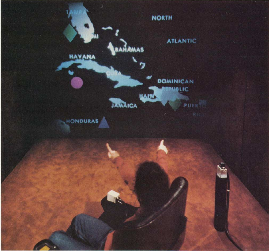
\includegraphics[width=5cm, keepaspectratio]{img/img1.png}
	\caption[Bolt's Put-That-There]{Bolt's Put-That-There from
	~\cite{turk_multimodal_2014}.}
	\label{fig:bolt}
    \captionvspace
\end{center}
\end{figure}

Regarding multiuser interactions, but without considering multimodal features,
some applications can increase the number of interacting users. However,
increasing the number of users does not necessary imply that the system has
become able to identify or distinguish each one of them, \textit{i.e.}~, it does not mean
that the system is fully aware of multiuser interactions. Stefik
~\cite{stefik_wysiwis_1987} proposes the early paradigm of WYSIWIS (What You See
Is What I See). This paradigm enables users to collaborate using the same GUI
across multiple users’ screens. Applications in this paradigm commonly use
shared view tools (\textit{e.g.} VNC--Virtual Network Computing--), and even when multiple users are interacting with
the system, the interacting users are not distinguished and are handled as if they were a single. More recently, research on 
Tabletop~\cite{muller-tomfelde_introduction:_2010} and DUI (Distributed
User Interfaces)~\cite{elmqvist_distributed_2011} has been studying multiuser
interaction over shared GUIs, but only few~\cite{dietz_diamondtouch:_2001} of
them truly consider multiuser interactions.

Truly multiuser applications are those in which the system can distinguish, and
the programmer is aware of, the different users who are interacting with the
system~\cite{haber_modeling_2001}. Some authors \cite{laurillau} also call the 
interface of
such applications as Identity-aware User interfaces (IAUI). Examples of
application of these truly multiuser interactions are present in gaming and
virtual reality contexts. In these contexts, users are uniquely identified in
each interaction. In game contexts, for instance, users use gamepad or motion
sensors (as illustrated in \fig{fig:multiuser}). 

\begin{figure}[!ht]
\begin{center}
	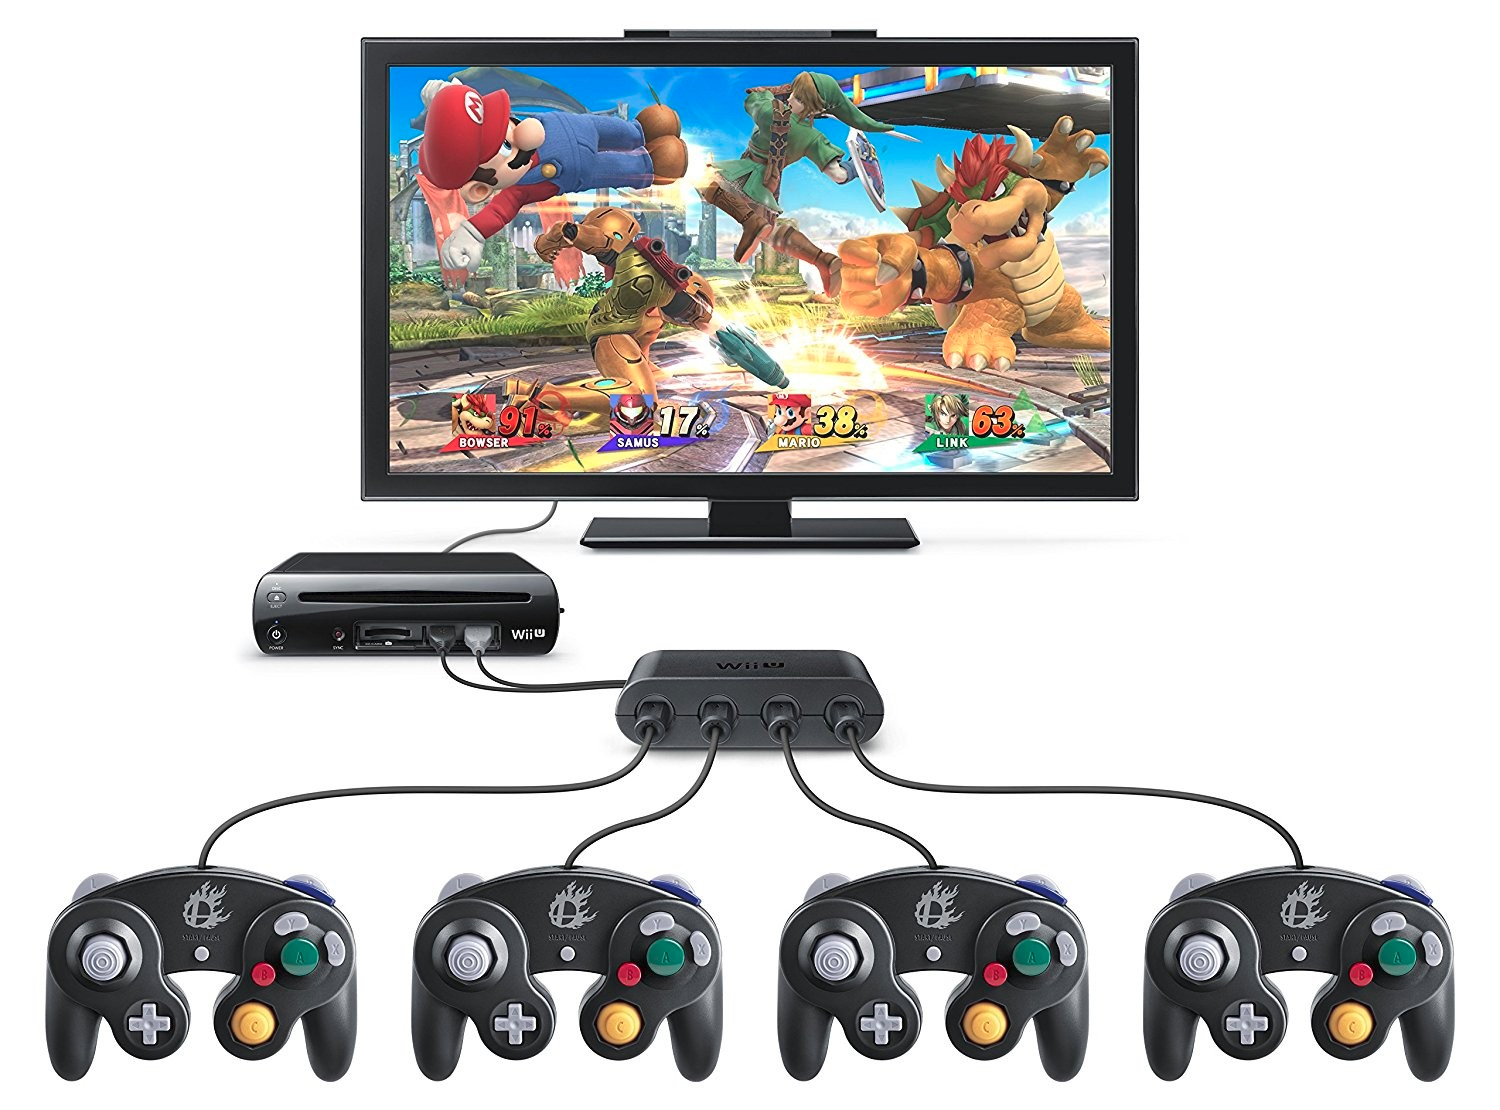
\includegraphics[width=5.5cm, keepaspectratio]{img/img2a.png}
	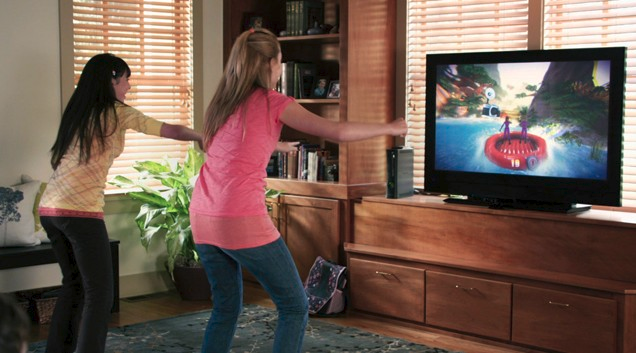
\includegraphics[width=7cm, keepaspectratio]{img/img2b.png}
	\caption[Multiuser games]{Multiuser games with GameCube
	gamepads\footnotemark and Microsoft Kinect\footnotemark}
	\label{fig:multiuser}
    \captionvspace
\end{center}
\end{figure}

\footnotetext[3]{\url{https://images-na.ssl-images-amazon.com/images/I/91Bs1LePe4L._SL1500_.jpg}}
\footnotetext[4]{\url{http://kinectmediaplayerassets.blob.core.windows.net/assets/contexts/adventures/thumb/thumb_kinect_adventures.jpg}}

This thesis addresses development of scenarios that use of human-computer
interaction possibilities, namely MUI and multiuser. To highlight such
scenarios, we present as follows some envisaged ones and their requirements.

\section{Envisaged scenarios and requirements}
\label{sec:intro:scenarios}

Based on Bolt’s scenario, \fig{fig:scenarios} presents the eight envisaged
scenarios of applications that use both multimodal and multiuser interactions.
We organize them by two categories, namely: “Put-That-There”
(\fig{fig:scenarios}-A to D) and “I-Get-That-You-Put-It-There”
(\fig{fig:scenarios}-E to H). Descriptions at the bottom of each scenario follow
the scheme: <number of output modalities, number of input modalities, and number
of interacting users>. We discuss each of them in what follows.

\begin{figure}[!ht]
\begin{center}
    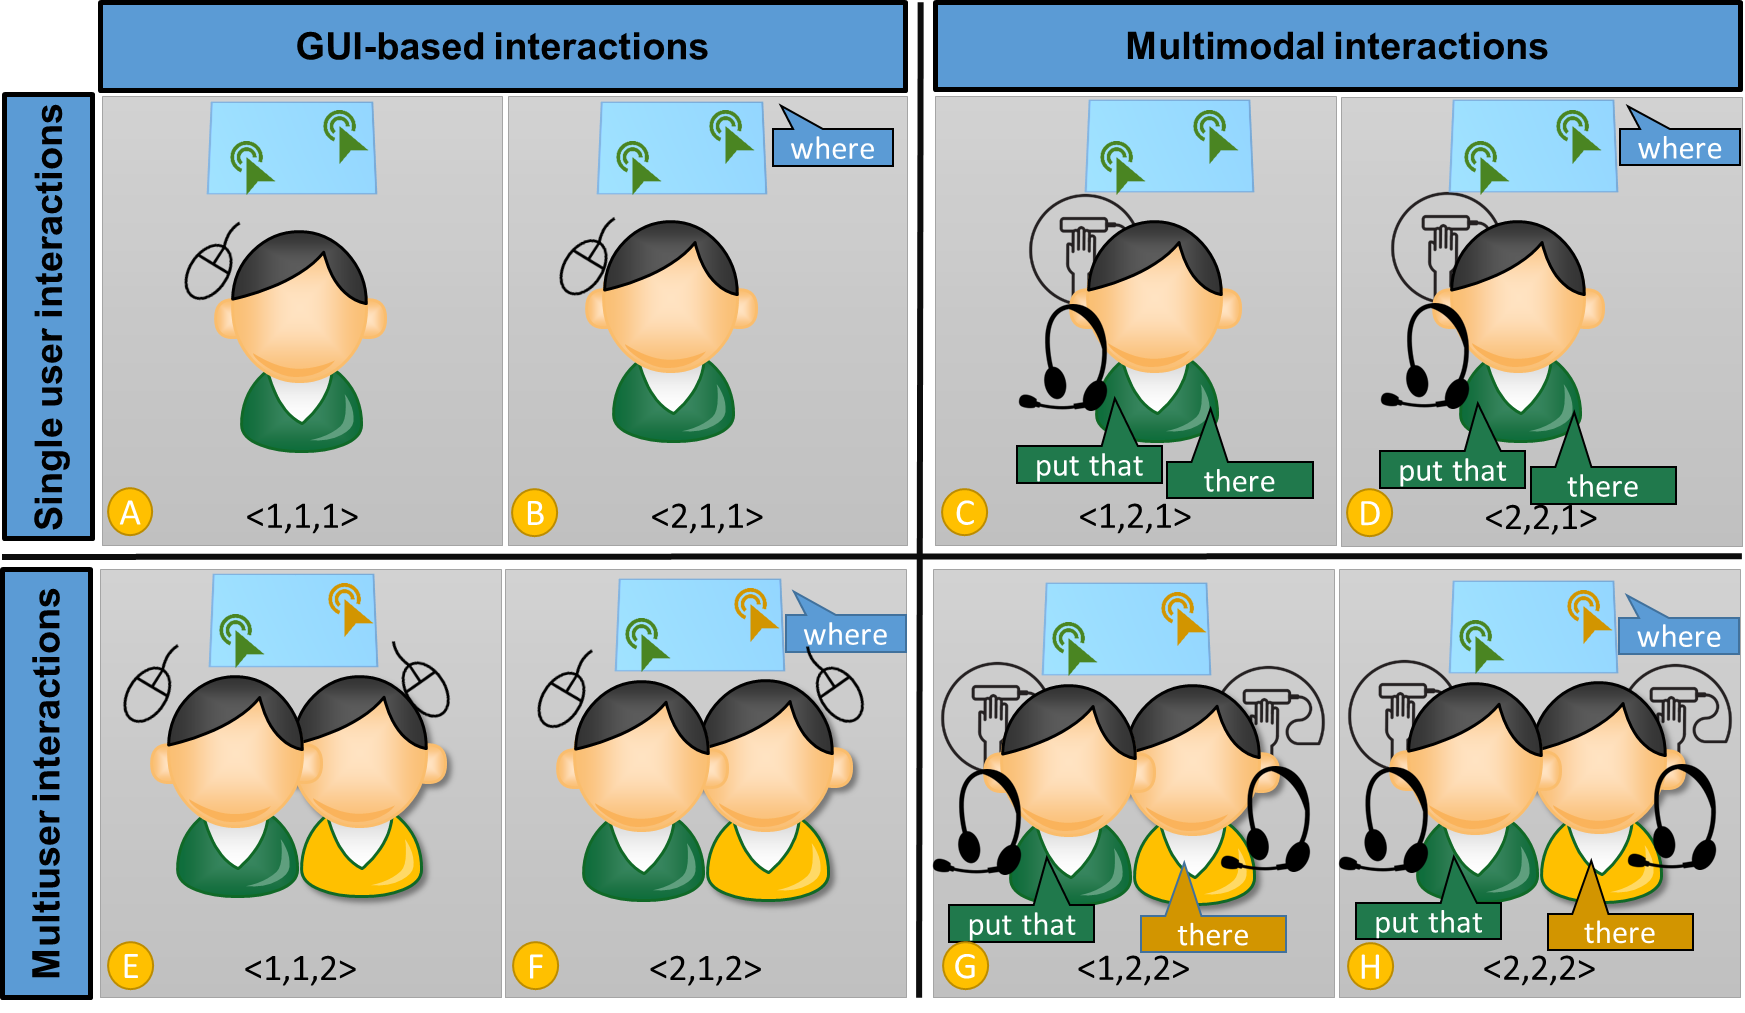
\includegraphics[width=12cm, keepaspectratio]{img/img3.png}
	\caption [Scenarios based on Bolt's Put-that-there]{Scenarios based on
		Bolt's Put-that-there with single/multiple output/input modalities and
		interacting users.}
    \captionvspace
	\label{fig:scenarios}
\end{center}
\end{figure}

The “Put-That-There” category is illustrated in \fig{fig:scenarios}-A to D. It
aims at varying the number of input and/or output modalities for a single user
interacting with the system. While \fig{fig:scenarios}-A and B use GUI-based
interactions, \fig{fig:scenarios}-C and D use multimodal interactions. In 
\fig{fig:scenarios}-A, the user interacts using a mouse and gets feedback on a
screen (one input and one output modality). \fig{fig:scenarios}-B extends A with
voice feedback (one additional output modality). In \fig{fig:scenarios}-C, the
user interacts using gestures and voice commands (two input modalities and one
output modality). \fig{fig:scenarios}-D extends C with voice feedback (two input
and two output modalities); it is similar to the original “Put-That-There”. Note
that these scenarios focus on supporting multimodal input/output for a single
user.

The “I-Get-That-You-Put-It-There” category is illustrated in
\fig{fig:scenarios}-E to \fig{fig:scenarios}-H. It is similar to the previous
“Put-That-There”, but the task must be performed by two different users, who are
uniquely identified when interacting with the system. When \fig{fig:scenarios}-E
and \fig{fig:scenarios}-F use GUI-based interactions, \fig{fig:scenarios}-G and
\fig{fig:scenarios}-H use multimodal interactions. \fig{fig:scenarios}-E shows
each user interacting through individual mice. \fig{fig:scenarios}-F extends the
previous one with voice feedback. \fig{fig:scenarios}-G shows each user
interacting through gestures and voice commands. \fig{fig:scenarios}-H extends
the previous one with voice feedback (\textit{i.e.}~, it is similar to the original
“Put-That-There”, but for two users). The “I-Get-That-You-Put-It-There” scenario
can be extended to handle users that are intentionally defined at runtime. For
instance, one may define that the first interaction (\textit{i.e.}~ point and 
say “put that”) is carried out by any user and the second interaction 
(\textit{i.e.}~ point and say “there”) by a different user. We name this variation as “Anyone-Get-That-Someone-Else-Put-It-There”.

The development of applications for the above scenarios brings both
specification and system requirements.

System must support:

\begin{itemize}	
	\item The synchronized presentation of audiovisual media objects. This
	synchronized presentation is required to maintain a coherent visual feedback
	of a MUI-interface;
	\item The presentation of synthesized media objects. MUI interfaces use output
	modalities that are synthesized in presentation time such as synthesized
	audio, avatar or send actions to actuators;
	\item Different input devices. As mentioned, devices such as microphone,
	motion sensors and gamepad may be used by the interacting users;
	\item The matching of the required user characteristics defined by the
	developer with the interacting users. Given the specification of the users
	capable of interacting with application, the system must verify whether a user
	can interact with the application.
\end{itemize}

The specification must support:

\begin{itemize}	
	\item Abstractions to use different output and input modalities, besides the
	traditional GUI-based ones. MUI interfaces use output modalities such as:
	synthesized audio, animated avatar, and sensorial effects. Those interfaces
	also use input modalities, such as gesture and speech recognition;
	\item The specification of combined behavior of output and input modalities.
	This support enables the orchestration of both input and output modalities;
	\item Abstractions to define how users should be capable of interacting with
	the application. This support enables the developer to define the
	characteristics users need to have to be able to interact with the
	application. In the Put-That-There scenario, for instance, the developer needs
	to specify that a user needs to have a gesture sensor and a microphone. 
\end{itemize}

In this thesis, we focus mainly on the specification requirements above to
define our research goal.

\section{Research goal}
\label{sec:intro:goal}

Given the aforementioned usage scenarios and their specification requirements,
this thesis addresses the following general research question:

\begin{quote}
	\textit{RQ1: How can we support the specification of applications that handle
	both multimodal interactions and multiple interacting users?}
\end{quote}

Some 
researches~\cite{dumas_description_2010,katsurada_xisl:_2005,w3c_multimodal_2003}
in Human-Computer Interaction (HCI) also address
this question, but they suffer from some relevant drawbacks (discussed in
\sect{chp:state}). In particular, they lack support for fine synchronization
among modalities. Synchronization among modalities is an issue mainly addressed
by Visualization and Multimedia (VMM) research. Thus, we address this question
by integrating efforts from both HCI and VMM. 

In fact, other researchers, such as Rowe~\cite{rowe_looking_2013} and Turk
~\cite{turk_multimodal_2014}, also share our motivation. Rowe’s 2013 ACM SIGMM
Report~\cite{rowe_looking_2013} claimed that multimedia applications with MUI
will be one of main themes for Multimedia research in the next few years.
Additionally, Turk~\cite{turk_multimodal_2014} argued that MUI is a
multidisciplinary object of study. The specification of recognizers and
usability of MUIs are commonly the focus of HCI research, while the
synchronization and development of output modalities are usually the focus of
VMM research. In particularly, VMM research addresses the specification of
synchronization by studies in multimedia languages.

Traditionally, those languages focus on specifying multimedia applications with
synchronized audiovisual media and limited user interactions. Examples of these
languages are: HTML5~\cite{w3c_html_2014}, NCL~(Nested Context Language)~\cite{abnt_abnt_2016}, and SMIL~(Synchronized
Multimedia Integration Language)~\cite{bulterman_smil_2008}. The developer who uses such languages is
usually called author. \fig{fig:overview-multimedia} illustrates an author
creating a multimedia application, and the multimedia system executing it. At
creation time, the author can use abstractions for: media, such as text (\textit{e.g.}~
HTML’s <p>, SMIL’s <text>), graphics (\textit{e.g.} HTML’s <img>), and videos 
(\textit{e.g.} HTML’s
<video>); synchronization; and user interactions mainly using mouse 
(\textit{e.g.} HTML’s
onClick, NCL’s onSelection) and keyboard (\textit{e.g.} HTML and SMIL’s 
keyPress, and
NCL’s onKeySelection). At execution time, the multimedia system presents the
media’s resulting content using audiovisual devices and reacts to pointer and
key-based user interactions.

\begin{figure}[!ht]
\begin{center}
	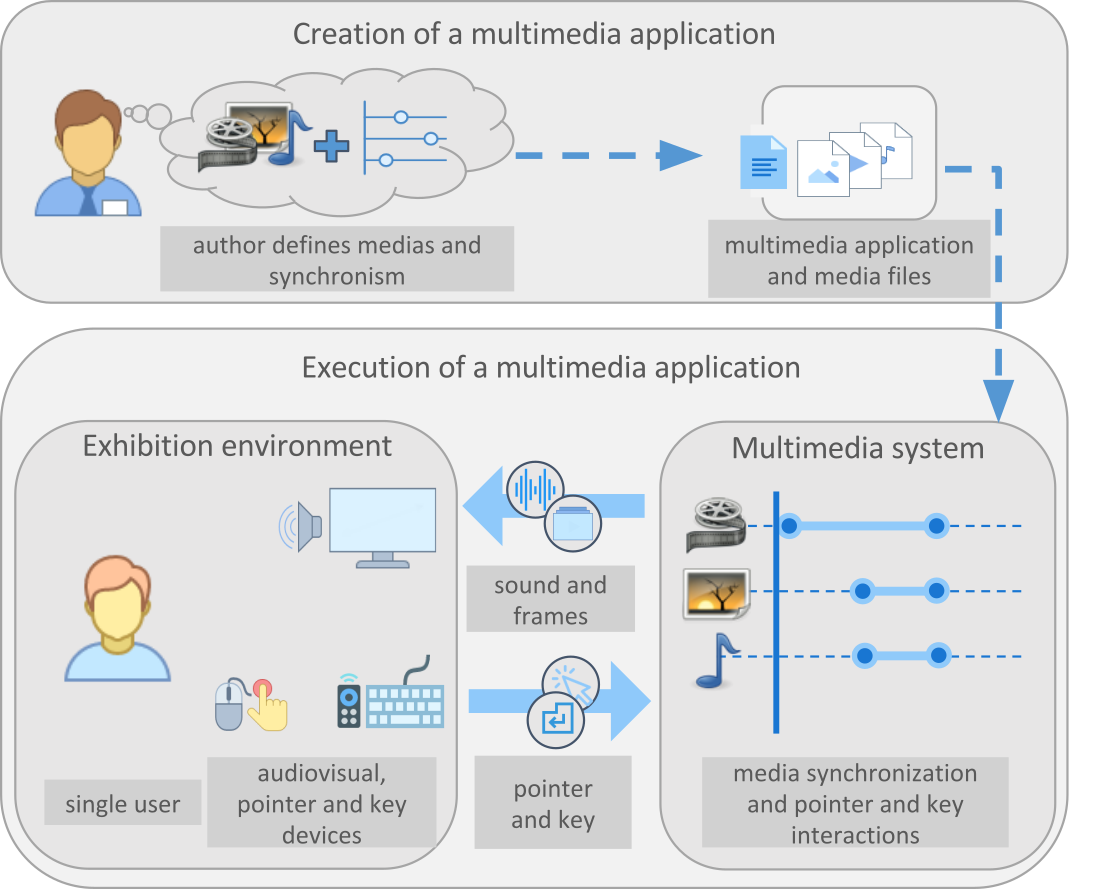
\includegraphics[width=10cm, keepaspectratio]{img/img4.png}
	\caption{Creation and execution of a multimedia application.}
    \captionvspace
	\label{fig:overview-multimedia}
\end{center}
\end{figure}

Given this context of multimedia languages, we argue throughout our research
that the support required by the \textit{RQ1} can be achieved by extending
multimedia languages to support multimodal and multiuser interactions.
Therefore, we define a more specific question to be addressed in this thesis:

\begin{quote}
	\textit{RQ2: How can we extend the output-oriented development in multimedia
	languages to handle multiple modalities of user interactions, besides the
	ordinary GUI-based ones, and multiple interacting users?}
\end{quote}

As discussed in \chp{chp:approach}, our approach proposes extensions to
multimedia languages with first-class entities to support both multimodal and
multiuser features. \fig{fig:overview-multimodal} illustrates our approach as a
new version of the previous figure. At creation time, the author can define not
only the media objects and the synchronization among them, but also the
multimodal and multiuser interactions. For instance, for multimodal
interactions, the author can specify a multimodal description, such as speech
recognition and gesture recognition descriptions. At execution time, the
multimedia system continues to use audiovisual devices to display the content of
the media and pointer/key devices to capture user interactions, but it also uses
multimodal interaction devices. For new output modalities, the multimedia can
also use actuators, which perform sensorial effects, and sensors, which perform
recognitions given multimodal descriptions.

\begin{figure}[!ht]
\begin{center}
	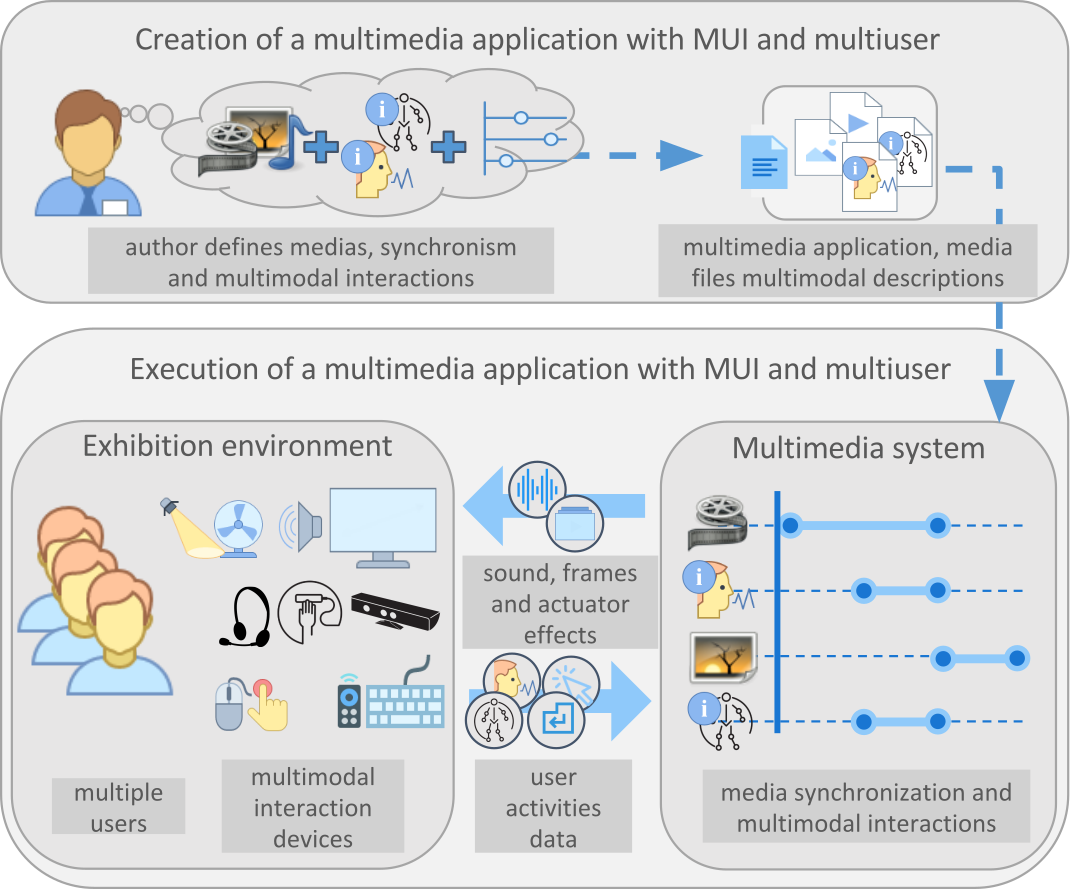
\includegraphics[width=10cm, keepaspectratio]{img/img5.png}
	\caption{Creation and execution of a multimedia application with multimodal
	and multiuser interactions.}
    \captionvspace
	\label{fig:overview-multimodal}
\end{center}
\end{figure}

Some works have aimed at extending multimedia languages (\textit{i.e.}~, those exemplified
in \fig{fig:scenarios}-A to 1-D). However, those works usually add only one new
modality to the language, usually speech
~\cite{beckham_towards_2001,carvalho_architectures_2008,
carvalho_estendendo_2010,	w3c_xhtml+voice_2001,wang_salt:_2002}. The next
chapter briefly discusses those works. To the best of our knowledge, no previous
work has proposed abstractions to support the specification of applications
using both multimodal and multiuser features. 

\section{Thesis structure}
\label{sec:intro:structure}

The remainder of this thesis is structured as follows. \chp{chp:state} presents
the related works, languages, and frameworks for the development of multimodal
and multiuser user interfaces, and highlights the main drawbacks of current
approaches. \chp{chp:approach} details our proposed approach to extend
multimedia languages, which overcomes the identified drawbacks.
\chp{chp:instantiation} presents instantiations of the proposed approach in NCL
and HTML languages. \chp{chp:evaluation} presents an evaluation of our proposal.
Finally, \chp{chp:final} presents our final remarks.

%%%%%%%%%%%%%%%%%%%%%%%%%%%%%%%%%%%%%%%%%%%%%%%%%%%%%%%%%%%%%%%%%%%%%%%%%%%%%%%%
\chapter{State of art}
%%%%%%%%%%%%%%%%%%%%%%%%%%%%%%%%%%%%%%%%%%%%%%%%%%%%%%%%%%%%%%%%%%%%%%%%%%%%%%%%
\label{chp:state} In this section, we present previous works that also aim at
supporting the development of multimodal (\sect{sec:state:multimodal}) and
multiuser (\sect{sec:state:multiuser}) interactions. Then, we summarize their
drawbacks (\sect{sec:state:drawbacks}).

\section{Support for multimodal interactions}
\label{sec:state:multimodal}

In order to guide our discussion about the support of multimodal interactions,
we present Dumas’s abstract architecture for MUI systems
~\cite{dumas_multimodal_2009} in what follows.

Dumas’s architecture (illustrated in \fig{fig:dulmas}) presents a MUI as a
perceptions-actions cycle between the multimodal system and the user. The user
performs actions through human communication activities (\textit{e.g.} speech, gestures,
touch) and perceives the (result of) system actions through stimuli to her/his
senses (\textit{e.g.} sight, hearing). We detail the key components of the architecture in
what follows.

\begin{figure}[!ht]
\begin{center}
	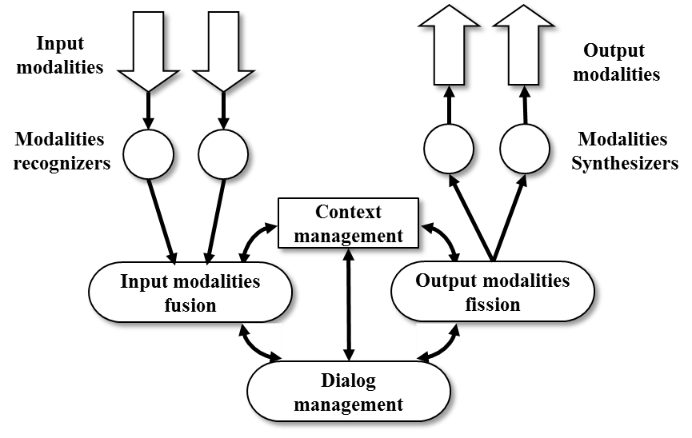
\includegraphics[width=10cm, keepaspectratio]{img/img6.png}
	\caption[Conceptual architecture of a multimodal system]{Conceptual 
	architecture of a multimodal system, adapted from~\cite{dumas_multimodal_2009}.}
	\label{fig:dulmas}
    \captionvspace
\end{center}
\end{figure}

\textit{Modalities recognizers} are capable of decoding \textit{input
modalities} through input devices and sensors (\textit{e.g.} keyboard, video camera, and
microphone). For example, an ASR (Audio Speech Recognition) recognizer
identifies sentences in audio samples captured by a microphone.
\textit{Modalities synthesizers} are capable of producing \textit{output
modalities} through audiovisual output devices and actuator devices (\textit{e.g.}~
monitor, speakers, haptic). For instance, a TTS (Text-To-Speech) synthesizer
produces audio to be played by a speaker.

\textit{Input modalities fusion} is the process of combining the recognizers’
results to interpret the user actions. For instance, fusion should interpret a
user text conveyed in either a speech or an ink modality. In addition, the
fusion should consider contextual information; for instance, it should not
expect voice commands from a speech-impaired user or when the user is in a loud
environment. 

\textit{Output modalities fission} is the generation of a system message --a
combination of actions in one or more synthesizers-- conveyed to the user
through certain output modalities. The choice of which modalities are used in
the message is called \textit{modality selection}, which must also consider
contextual information —\textit{e.g.} it would not make sense to use visual modalities to
convey information to a blind user. 

\textit{Dialog management} maintains the communication flow between the user 
and the system. The dialog defines a combination of fission and fusion 
processes, performed at each moment of application behavior. Finally, 
\textit{context management} is responsible for storing the user context 
(\textit{e.g.} car, mobile, home) and profile (\textit{e.g.} blind, deaf, 
mute), which enables the fission and fusion processes to be adapted. In view 
the of Dumas’s architecture, we discuss four groups of works in the next 
subsections (from \ref{sec:state:monomodal} to \ref{sec:state:multimedia}). As 
illustrated in \tab{table:state}, each group supports some parts of the Dumas’s 
architecture. 

\begin{landscape}
\centering	
\begin{table}
\scriptsize
\def\arraystretch{2}
%\resizebox{24cm}{!}{%
\begin{tabular}[]{ m{4cm}|m{3cm} m{3cm} m{3cm} m{3cm} m{3cm} m{3cm}}

	%%%%%% 
	\hline
	\textbf{Approach} 
		& \textbf{Recognizers}
		& \textbf{Fusion}
		& \textbf{Dialog \newline management}
		& \textbf{Context \newline management}
		& \textbf{Fission}
		& \textbf{Synthesizers} \\
	\hline

	%%%%%% 
	\hline
	\rowcolor[HTML]{F2F2F2} \multicolumn{7}{c}{Language used by either 
	recognizers or synthesizers}\\
	\hline
	
	\textbf{SRGS~\cite{andrew_hunt_speech_2004}, InkXML~\cite{w3c_ink_2011}, GDL~\cite{hachaj_semantic_2012}, and GML~\cite{ideum_inc_gesture_2016}} & 
	specialized 
	modality & sequential-only & & & \\
	\textbf{SSML~\cite{daniel_c._burnett_speech_2010}, 
	BML~\cite{vilhjalmsson_behavior_2007}, and 
	SEDL~\cite{iso/iec_iso/iec_2013}} & & & & & specialized 
	modality & 
	sequential-only\\
	\hline

	%%%%%%		 
	\rowcolor[HTML]{F2F2F2} \multicolumn{7}{c}{Form-based dialog languages}\\
	\hline
	
	\textbf{VoiceXML~\cite{w3c_voice_2007} and SALT 
	~\cite{microsoft_speech_2003}} & speech & sequential-only & 
	form-based & & sequential-only & speech \\
	\textbf{XISL~\cite{katsurada_xisl:_2005}} & agnostic <input> element	& 
	SMIL 
	\textit{seq},\textit{par} and \textit{alt} operators & form-based & & SMIL 
	seq, par and alt operators & agnostic <output> element \\
	\hline
	
	%%%%%% 
	\hline
	\rowcolor[HTML]{F2F2F2} \multicolumn{7}{c}{Frameworks}\\
	\hline
	
	\textbf{MMI~\cite{w3c_multimodal_2003}} & MCs with LifeCycle messages & DoneNotification with EMMA 
	& state machine\newline(SCXML) & SCXML \newline (ECMAScript) & sequence of 
	LifeCycle messages (optionally inside if-then-else) & MCs with LifeCycle 
	messages \\
	\textbf{HephaticsTK~\cite{dumas_description_2010}} & SMUIML \newline agnostic <recognizer> element & 
	CARE properties based operators & state machine (SMUIML) & & SMUIML 
	sequence of <result> elements & ad-hoc message\\
	\hline

	%%%%%% 
	\hline
	\rowcolor[HTML]{F2F2F2} \multicolumn{7}{c}{Multimedia languages}\\
	\hline
	
	\textbf{HTML+SALT~\cite{wang_salt:_2002} and HTML+ VoiceXML~\cite{w3c_xhtml+voice_2001}} & key/pointer+ 
	VoiceXML & &  
	low-level (JavaScript) & & & text, image, video, and audio elements\\
	\textbf{SMIL+Rex~\cite{beckham_towards_2001}} & key/pointer+ VoiceXML & & low-level (par and seq 
	time 
	containers) & & seq, par, excl time containers & text, image, video and 
	audio elements\\
	\textbf{NCL+VoiceXML~\cite{carvalho_estendendo_2010}} & key/pointer+ VoiceXML & & low-level (causality 
	links) & user and system variables & seq operators with media, switch, and 
	anchors & agnostic media element\\
	\hline
	
\end{tabular}
%}
\caption{Comparison among the features supported by the different MUI 
development approaches.}
\label{table:state}
\end{table}
\end{landscape}

\subsection{Languages used by recognizers and synthesizers}
\label{sec:state:monomodal}

The first group of related work consists of languages that handle either only 
\textit{recognizers} or only \textit{synthesizers}. None of them supports dialog
or context management.

SRGS (Speech Recognition Grammar Specification)~\cite{andrew_hunt_speech_2004},
InkXML (Ink Markup Language)~\cite{w3c_ink_2011}, GDL (Gesture Description
Language)~\cite{hachaj_semantic_2012}, and GML (Gesture Markup Language)
~\cite{ideum_inc_gesture_2016} assist in describing \textit{recognizers}. SRGS
is a grammar format for speech recognition. InkXML is a representation for
electronic ink created with a stylus or other pointing devices, useful for
handling text input. Finally, GDL and GML focus on describing user movements:
GDL describes body joint movements captured by sensors (\textit{e.g.} Microsoft Kinect),
and GML focuses on touch gestures captured by touchpad devices.

SSML (Speech Synthesis Markup Language)~\cite{daniel_c._burnett_speech_2010},
BML (Behavior Markup Language)~\cite{vilhjalmsson_behavior_2007}, and SEDL
(Sensory Effect Description Language)~\cite{iso/iec_iso/iec_2013} assist in
describing \textit{synthesizers}. SSML is a representation for pronunciations
focused on text-to-speech engines and can control speech aspects (\textit{e.g.}~
pronunciation, volume, rate, pitch, and rhythm). BML enables controlling the
verbal and nonverbal behavior of embodied conversational, useful for children-
or elderly-oriented MUIs. Finally, SEDL, part of the MPEG-V framework
~\cite{iso/iec_iso/iec_2014}, supports the description of sensory effects such
as light, wind, fog, and chair vibration, which can be useful to enhance the
consumer’s experience of an audiovisual content.

\subsection{Form-based dialog languages}
\label{sec:state:dialog}

The second group of related work consists of languages that focus on specifying
the dialog management through a form-based approach. More precisely, developers
specify MUI systems through questions, to be conveyed by the system through
synthesizers, and expected answers from the user, interpreted through
recognizers. None of the works in this group supports context management.

VoiceXML (Voice Extensible Markup Language)~\cite{w3c_voice_2007} and SALT
(Speech Application Language Tags)~\cite{microsoft_speech_2003} are limited
to speech modalities and the widely used development of vocal interactions
focusing on telephony conversations. They can use synthesized speech and
digitized audio (voice recordings) as output. In addition, they can recognize
speech and telephony DTMF (Dual-Tone Multi-Frequency) digits as input. Both
focus on speech-only conversations, providing elements such as <listen> and
<prompt>. In those languages, the author only combines a sequence of input or a
sequence of output modalities.

XISL (eXtensible Interaction Scenario Language)~\cite{katsurada_xisl:_2005} 
introduces an agnostic
treatment for modalities through the <input> and <output> elements. It is
inspired by the VoiceXML dialog but uses SMIL <par> and <seq> elements for
defining the modalities synchronization. The XISL dialog uses a <prompt> element
for system questions, <operation> for the fusion of user inputs, and <action>
for the fission of outputs —\textit{i.e.}~, the system response. Inside fusion (\textit{i.e.}~
<operation>) or fission (\textit{i.e.}~ <action>), XSI supports temporal relationships
through the <par> and <seq> SMIL elements, which are children of the <operation>
and <action> elements. 

\subsection{Frameworks}
\label{sec:state:frameworks}

The third group of related work consists of frameworks that focus on specifying
the dialog management, usually using state machines. Those frameworks delegate
the fission to be handled by a multimedia system. For instance, fine media
synchronization, such as lip-syncs, are delegated to the multimedia system.

W3C’s MMI (Multimodal Interaction)~\cite{w3c_multimodal_2003} framework is
defined by Modality Components (MCs) and an Interaction Manager (IM). Inspired
by XISL, an MC is modality agnostic and it is responsible for one or more input
or output modalities, which it can handle by nesting other MCs and IMs. The IM
controls the dialog flow of the application by coordinating the MCs by message
exchange using an API named Life-Cycle~\cite{w3c_multimodal_2012}. These
messages include the activation of an MC (\textit{e.g.} Start, Pause, Cancel) and the
result of an MC by a DoneNotification (\textit{e.g.} end of speech recognition). MMI is
instantiated by \textit{control} and 
\textit{presentation} documents, which implement IM and MCs, respectively. MMI
recommends the use of SCXML~\cite{w3c_state_2012} for control documents, and
VoiceXML, HTML, or SMIL for presentation documents. \fig{fig:mmi} illustrates
the message exchange between control and presentation documents. An SCXML
document describes the multimodal dialog using state machines, in which a set of
<state> and <transition> elements defines the possible states of the multimodal
application and the transitions between them. When transitioning between states,
SCXML sends life-cycle events to MCs. Additionally, these transitions can use
“if-then-else” constructions and ECMAScript variables. MMI recommends EMMA
(Extensible MultiModal Annotation markup language)~\cite{w3c_emma:_2009} to
describe DoneNotification messages exchanged between presentation documents and
their IM. EMMA defines a semantic interpretation for a variety of modalities;
for instance, presentation documents can interpret a text input in either a
speech or an ink modality.

\begin{figure}[!ht]
\begin{center}
	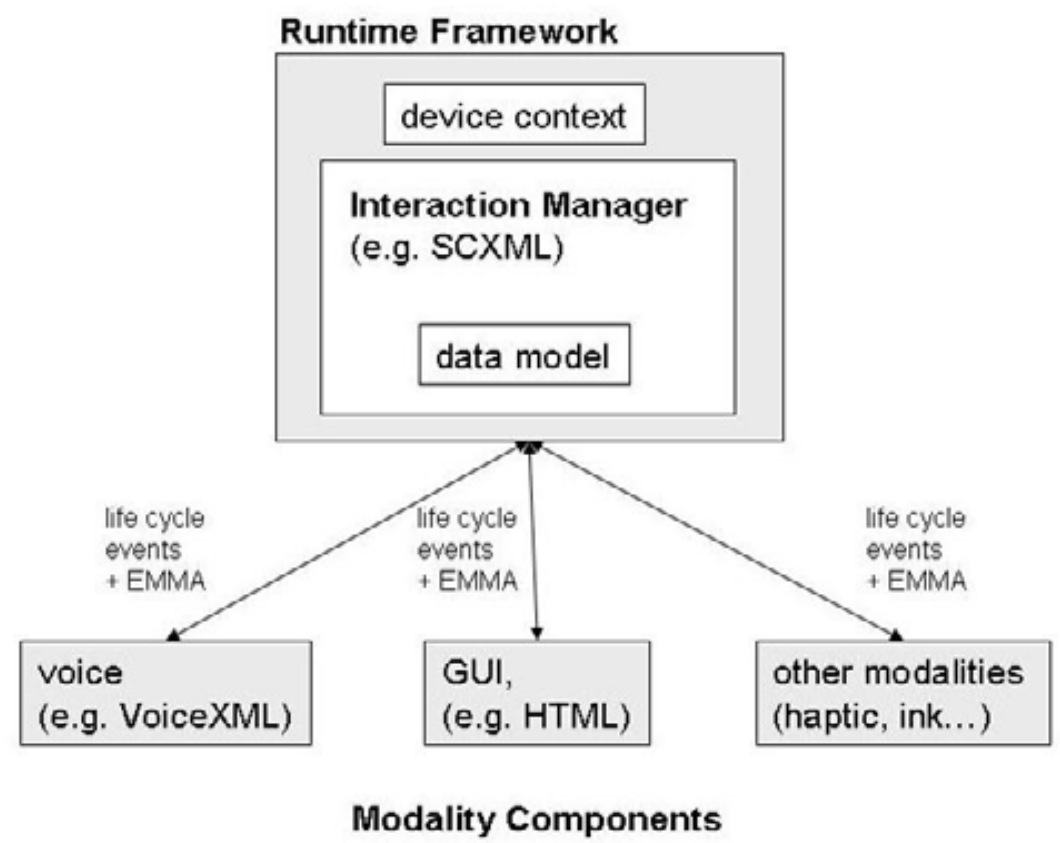
\includegraphics[width=5cm, keepaspectratio]{img/img7.png}
	\caption[MMI overview]{MMI overview, from~\cite{dahl_standards_2009}.}
	\label{fig:mmi}
	\captionvspace
\end{center}
\end{figure}

Aiming at implementing his architecture, Dumas proposes the HephaticsTK 
framework. This framework is instantiated by one SMUIML (Synchronized 
Multimodal User Interaction Modeling Language)~\cite{dumas_description_2010} document and its client 
application. Illustrated in \fig{fig:smuiml}, SMUIML is a state-machine-based 
language 
that focuses on the specification of the fusion process. HephaticsTK delegates 
the fission to the client application in charge of interpreting the message and 
generating one or more output modalities. 

\begin{figure}[!ht]
\begin{center}
	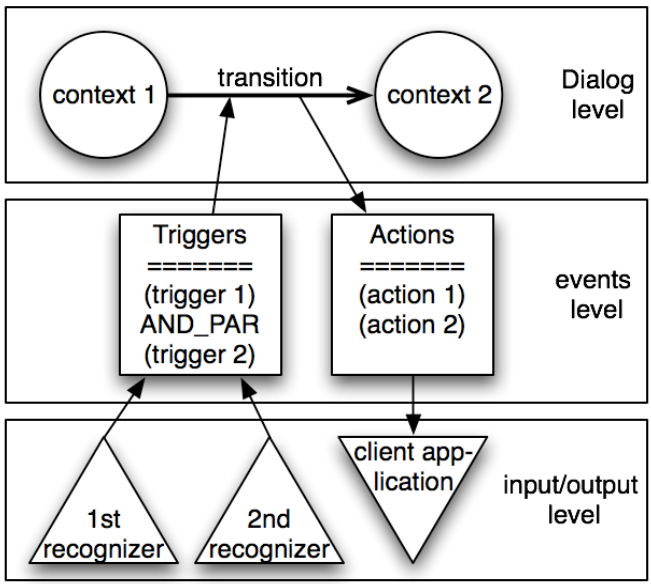
\includegraphics[width=5cm, keepaspectratio]{img/img8.png}
	\caption[SMUIML overview]{SMUIML overview, from~\cite{dumas_prototyping_2008}.}
	\label{fig:smuiml}
    \captionvspace
\end{center}
\end{figure}

In an SMUIML document, a state transition (<transition> element) is defined
through a combination of recognizers’ results (<triggers>) and messages to be
sent to the client application (<action>). This combination process of SMUIML
considers the CARE (\textit{Complementarity}, \textit{Assignment}, 
\textit{Redundancy}, and \textit{Equivalence}) properties~\cite{coutaz_four_1995}. 

The formal expressions of the CARE properties rely on the transitions between
two states of a given multimodal system. Considering S’ following S, 
\textit{Assignment} expresses the absence of choice: a single modality is
available in S to reach S’. \textit{Equivalence} means the availability of
choice between multiple modalities, \textit{i.e.}~, the use of any one of the modalities is
enough to reach state S’ from state S. \textit{Redundancy} means that a set of
modalities are used redundantly to reach S’ from S, \textit{i.e.}~, when they are used
within the same temporal window without increasing the user’s expressive power.
A set of modalities is used in a \textit{Complementary} way within a temporal
window if all of them must be used to reach S’ from S, either sequentially or in
parallel. \sect{sec:state:allen} discusses the state of the art in 
terms of combination of modalities and their expressiveness. 

SMUIML implements CARE assignment by using only one <trigger> per <transition>.
To implement the remainder CARE properties, SMUIML proposes four elements to
combine the <trigger>s: <par\_and> (CARE \textit{parallel Complementarity});
<seq\_and> (CARE \textit{sequential Complementarity}); <par\_or> (CARE
\textit{Redundancy}); and <seq\_or> (CARE \textit{Equivalence}). 
\lis{list:smuiml} shows the “Put-that-there” in SMUIML, which uses <seq\_and> 
and <par\_and> combinations.

\begin{listing}
\begin{minted}[linenos,fontsize=\scriptsize,numbersep=1pt,frame=lines,xleftmargin=10pt,framesep=2mm]{xml}
<transition leadtime="1500">
<seq_and>
  <trigger name="put_trigger" />
  <transition>
  <par_and>
    <trigger name="that_trigger" />
    <trigger name="object_pointed_event" />
  </par_and>
  </transition>
  <transition>
  <par_and>
    <trigger name="there_trigger" />
    <trigger name="object_pointed_event" />
  </par_and>
  </transition>
</seq_and>
<result action="put_that_there_action" />
</transition>
\end{minted}
\caption[“Put-that-there” expressed in SMUIML.]{“Put-that-there” example 
illustrating CARE properties, expressed in 
SMUIML. Adapted from~\cite{dumas_frameworks_2010}.}
\label{list:smuiml}
\end{listing}

\subsection{Multimedia languages}
\label{sec:state:multimedia}

Similar to our approach, some works
~\cite{beckham_towards_2001,carvalho_architectures_2008,
carvalho_estendendo_2010,	w3c_xhtml+voice_2001,wang_salt:_2002} extended XHTML
(eXtensible Hypertext Markup Language)~\cite{w3c_xhtml_2000}, SMIL, and NCL to
support multimodal interactions. The main drawback of these works, however, is
that they do not provide a way to seamlessly integrate new modalities, because
they incorporate recognizer specification by overloading existing elements or
adding directly into a multimedia language body. In particular, they are limited
to adding only a speech modality by incorporating VoiceXML and SALT elements.

Wang~\cite{wang_salt:_2002} proposes the integration of SALT elements
(\textit{e.g.} <salt:prompt>, <salt:grammar>) directly into XHTML. Likewise, 
W3C~\cite{w3c_xhtml+voice_2001} proposes the integration of VoiceXML elements
(\textit{e.g.} <vxml:prompt>,<vxml:grammar>) directly into XHTML. Both proposals
use DOM events or JavaScript code to support relationships between voice
recognition/synthesis with XHTML content. Those scripts allow developers to
control, in an imperative manner, the activation of recognizers and
synthesizers, as well as the notification of the recognizers’ result.

Beckham~\cite{beckham_towards_2001} proposes elements for integrating voice
recognition and synthesis in SMIL. For speech synthesis, Beckman proposes a
<TTS:render> element. For speech recognition, Beckman proposes a reactive
language, named REX (Reactive XML), which has <raise>, <handle>, and <await> as
its main elements. The <raise> element specifies the ASR (Audio Speech
recognition) grammar to be recognized; <handle> defines actions that must be
performed when a recognition grammar is accepted; and <await> acts as a <par>
composition which includes <raise> and <handle>. As with other related work,
Beckman’s proposal merges elements related to recognition and speech synthesis
with the specification of the multimedia document. Another drawback is the fact
that it only adds supports to recognition and synthesis of a single modality
(voice).

Carvalho \textit{et al.}~\cite{carvalho_architectures_2008,carvalho_estendendo_2010}
propose two approaches for integrating VoiceXML elements into NCL. They both
incorporate VoiceXML directly into the XML tree of an NCL document and then map
VoiceXML elements for voice recognition onto keyboard-based events of NCL. In
~\cite{carvalho_architectures_2008}, a VoiceXML dialog is inserted into the
<port> NCL element (\lis{list:carvalho1}) and is activated in the beginning of
the document, whereas in~\cite{carvalho_estendendo_2010} the dialogue is
inserted into the <link> element (\lis{list:carvalho2}) and is activated when
the media related with the <link> is occurring. Besides overloading the concept
of the <port> and <link> elements, these approaches compromise the separation
between the structure and the content of the application, which is favored by
the NCL model, namely NCM~\cite{soares_nested_2009}. Moreover, the proposals do
not allow developers to control the internal behavior of events occurring inside
the VoiceXML dialog, which prevents the creation of relationships between the
speech synthesis and recognition with other media objects.

\begin{listing}[!ht]
\begin{minted}[linenos,fontsize=\scriptsize,numbersep=1pt,frame=lines,xleftmargin=10pt,framesep=2mm]{xml}
<ncl>
  ...
  <body>
  <port id="pInicio" component="video">
    <voice>
      <menu scope="dia1og">
        <prompt>
          Video inicializado. Se deseja finalizar o video
          clique no botão<emphasy>vermelho</emphasy> ou diga
          <emphasy>SIM</emphasy>.
        </prompt>
        <choice next="#rec1">Sim</choice>
      </menu>
      <optionChoice id="rec1" action="RED" />
    </voice>
  </port>
  <media id="video" src="media/video.mpg" descriptor="dIV">
    <link id="iniciarVoz" xconnector="onSelectionStop">
      <bind component="video" ro1e="onSe1ection">
        <bindParam nae="keyCode" va1ue="RED" />
      </bind>
      <bind component="video" ro1e="stop"/>
      <voice>
        <prompt>Video finalizado</prompt>
      </voice>
    </link>
  </body>
  ...
</ncl>
\end{minted}
\caption[NCL using VXML inside an <port>.]{Code fragment 
from~\cite{carvalho_architectures_2008}, which uses VXML inside an <port>.}
\label{list:carvalho1}
\end{listing}

\begin{listing}[!ht]
\begin{minted}[linenos,fontsize=\scriptsize,numbersep=1pt,frame=lines,xleftmargin=10pt,framesep=2mm]{xml}
<link xconnector="onKeySelectionStartStop">
  <bind component="prato3" role="onSelection">
    <bindParam name="keyCode" value="GREEN"/>
  </bind>
  ...   
  <vncl>
    <prompt>
      To choose the dish with vegetables and fish, say: 
      <break size="medium"/>Green<break size="small"/>
      or meat and fried potatoes<break size="small"/>
    </prompt>
    <choice text="Dish with meat and fried potatoes.">
      <grammar type="text/gsl">[green vegetables fish]</grammar>
      <object action="GREEN" />
    </choice>
  </vncl>
</link>
\end{minted}
\caption[NCL using VXML inside an <link>.]{Code fragment 
from~\cite{carvalho_estendendo_2010}, which uses VXML inside an <link>.}
\label{list:carvalho2}
\end{listing}

The aforementioned works may specify dialog management through low-level
(multimedia-oriented) constructions of their languages. More specifically, to
support dialog management, HTML can use JavaScript, SMIL can use time
containers, and NCL can use causality links. Another characteristic of the
proposals in this group is that they already support audiovisual synthesizers.
In NCL, an agnostic <media> element is used, which is similar to the XISL
<output> element. Moreover, NCL supports context management using global
variables.

Although they do not directly address multimodal interactions, Moreno et 
al.~\cite{moreno_extending_2017} aim at extending NCM 3.0 and NCL 3.0 to 
support some kind of recognition.
Their proposal is inspired by semantics descriptions such as RDF (Resource Description Framework)~\cite{w3c_rdf/xml_2014} and proposes to
use <media> elements to describe abstract concepts (\textit{e.g.} soccer player and piece
of art). More precisely, in their proposal, an author may define abstract
concepts by: defining <media> elements with a string-based \textit{concept}
attribute and relating them using <spoConnector> (subject-predicate-object)
relations; or by defining <media> that refer to an RDF description (src
attribute). Once defined, these concepts can be recognized (\textit{inferFrom}
<link> role) in other <media> elements. For instance, \lis{list:moreno} 
illustrates the NCL code fragment of application that shows a museum tour 
video, and an additional content is presented when some specific piece of art 
appears in the video.

\begin{minted}[linenos,fontsize=\scriptsize,numbersep=1pt,frame=lines,xleftmargin=10pt,framesep=2mm]{xml}
<ncl>
  <head>
    <connectorBase>
      ...
      <spoConnector id="arts">
        <subject nole="subject" max="1"/>
        <compoundObject qualifier="seq">
          <simpleObject role="born" max="1"/>
          <simpleObject role="painted" max="unbounded" qualifier="seq"/>
        </compoundObject>
      </spoConnector>
      <spoConnector id="appearance">
        <subject nole="subject" max="1"/>
        <simpleObject nole="appears" max="unbounded" qualifier="seq"/>
      </spoConnector>
      <causalConnector id="onBeginInferFromStart">
        <compoundCondition>
          <simpleCondition role="onBegin"/>
          <inference role="inferFrom" qualifier="from"/>
        </compoundCondition>
        <simpleAction role="start" max="unbounded"/>
      </causalConnector>
    </connectorBase>
  </head>
  <body>
    <port id="p1" component="museum"/>
    <port id="p2" component="expo"/>
    <media id="museum" src="museum.mp4"/>
    <media id="expo" src="VanGoghExpo.mp4"/>
    <media id="imgl" src="sn1.jpg"/>
    <link id="l1" xconnector="onBeginFromstart">
      <bind role="onBegin" component="starry_night"/>
      <bind role="inferFrom" component="museum"/>
      <bind role="start" component="img1"/>
    </link>
    ...
    <media id="starry_night" concept="Starry Night"/>
    <media id="van_gogh" concept="Vincent Van Gogh"/>
    <media id="sn_canvas" src="images/starrynight.jpg"/>
    <media id="sn_museum" src="images/snmuseum.jpg"/>
    <link id="l5" xconnector="arts">
      <bind role="subject" component="van_gogh"/>
      <bind role="born" component="zundert"/>
      <bind role="painted" component="starry_night"/>
    </1ink>
    <link id="l6" xconnector="appearance">
      <bind role="subject" component="starry_night"/>
      <bind role="appears" component="sn_canvas"/>
      <bind role="appears" component="sn_museum"/>
    </link>
  </body>
</ncl>
\end{minted}

\begin{listing}[!ht]
    \caption[NCL code fragment for recognitions in video]{NCL code fragment for recognitions in video, adapted from~\cite{moreno_extending_2017}.}
    \captionvspace
    \label{list:moreno}
\end{listing}

\subsection{Expressiveness analysis}
\label{sec:state:allen}

Based on the Dumas’s architecture for multimodal systems, the previous
subsections discussed the support provided by current approaches for developing
MUIs. To highlight gaps of the related works in terms of their Expressiveness power, in this
section we analyze them based on Allen’s temporal relations. Allen’s relations 
were initially proposed to express
temporal relations among intervals in the database field
~\cite{allen_maintaining_1983}. In the Multimedia research, they are commonly
used to describe the temporal arrangement among media objects in a multimedia
presentation~\cite{huang_synchronization_1998}. 
\tab{table:allen} illustrates the seven temporal relations proposed by Allen. 

\begin{table}[b]
\scriptsize
\def\arraystretch{2}
\begin{tabular}{ l l l m{3cm} m{7cm} }
	\hline
	\multicolumn{3}{c}{\textbf{Allen’s relation}}
		& \textbf{Visual} \newline \textbf{representation} & 
		\textbf{Semantics}	\\
	\hline
	%%%%%% 
	T1 &	before &	T2 & 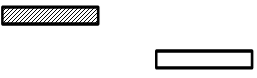
\includegraphics[width=1.5cm, 
	keepaspectratio]{img/allen1.png} 	& T1 takes place before T2 \\
	\hline
	T1 &	equals &	T2 &	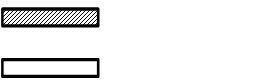
\includegraphics[width=1.5cm, 
	keepaspectratio]{img/allen2.png} & T1 is equal to T2 \\
	\hline
	T1 &	meets &	T2 &	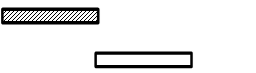
\includegraphics[width=1.5cm, 
	keepaspectratio]{img/allen3.png} & T1 meets T2 \\
	\hline
	T1 &	overlaps &	T2 &	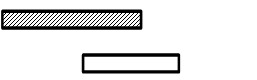
\includegraphics[width=1.5cm, 
	keepaspectratio]{img/allen4.png} & T1 starts before T2 and they overlap  \\
	\hline
	T1 &	during &	T2 &	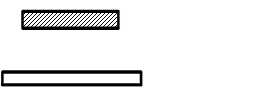
\includegraphics[width=1.5cm, 
	keepaspectratio]{img/allen5.png} & T1 is fully contained within T2 \\
	\hline
	T1 &	starts &	T2 &	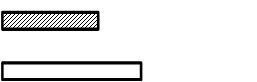
\includegraphics[width=1.5cm, 
	keepaspectratio]{img/allen6.png} & T1 starts together with T2 \\
	\hline
	T1 &	finishes &	T2 &	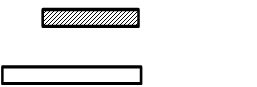
\includegraphics[width=1.5cm, 
	keepaspectratio]{img/allen7.png} & T1 finishes together with T2 \\
	\hline
\end{tabular}
\caption[Visual representations of Allen’s temporal relations.]{Visual 
representations of Allen’s temporal relations. Adapted 
from~\cite{allen_maintaining_1983}.}
\label{table:allen}
\end{table}

Different from previous analyses~\cite{huang_synchronization_1998}, which only
use Allen’s temporal relations for analyzing media objects (output modalities),
we use them for analyzing both output and input modalities. Here, the temporal
interval of an output or input modality means the interval in which it is
activated, \textit{i.e.}~ the time between its activation and its deactivation. 

\tab{table:allencomp} presents the analysis of the expressive power of the
selected approaches based on Allen’s temporal relations. In this analysis, for
each relation, we use every possible combination of input modalities (iM) and
output modalities (oM). Some of the works discussed in this \chp{chp:state} were 
excluded from the analysis because they do not handle fission and fusion 
together. The
excluded works are: the unimodal languages, such as SSML and SRGS; and the
form-based approaches specialized in only one modality, such as VoiceXML, SALT,
and MIML. In addition, we have excluded the HTML-based approaches, because they
lack an explicit specification of synchronization between output and input
modalities, delegating it to JavaScript.

XISL is a form-based language that expresses output modalities (\textit{i.e.}~ system
questions) followed by input modalities (\textit{i.e.}user answers), or 
vice-versa. This
means that it is possible to implicitly specify the “iM \textit{meets} oM” and
“oM \textit{meets} iM” relations. Moreover, XISL uses the SMIL operators
(\textit{seq} and 
\textit{par}) to combine a set of either output modalities or input modalities
(but not both input and output within a single set). The seq operator in input
modalities enables “iM \textit{meets} iM.” The \textit{seq} operator in output
modalities enables “oM \textit{meets} oM.” The \textit{par} operator in input
modalities enables “iM \textit{starts} iM.” The 
\textit{par} operator in output modalities enables “oM” \textit{starts} oM”.
Despite using the SMIL containers, XISL does not offer anchor attributes, such
as \textit{begin} and 
\textit{end}, which prevents it from expressing the \textit{before},
\textit{overlaps}, and 
\textit{during} relations. Finishes and equals are not supported either.

\begin{table}[!ht]
\scriptsize
%\def\arraystretch{1}
%\resizebox{\textwidth}{!}{%		
\begin{tabular}{ m{1.8cm} m{0.5cm} m{1cm} m{0.5cm} m{1cm} m{1cm} 
m{1.5cm} m{1.5cm} m{1.5cm}}
	%%%%%% 
	\hline
	& \multicolumn{3}{c}{\textbf{Allen’s relation}}
		& \textbf{XISL}	& \textbf{W3C MMI}	& \textbf{SMUIML}	& 
		\textbf{SMIL+} \newline \textbf{Rex}	& \textbf{NCL+} \newline 
		\textbf{VoiceXML} \\

	%%%%%% 
	\hline
	\multirow{7}{*}{fusion} 
	& iM &	before &		iM & & & & & \\
	& iM &	equals &		iM & & & Yes & & \\
	& iM &	meets &			iM & Yes & Yes & Yes & &\\
	& iM &	overlaps &	iM & & & & & \\
	& iM &	during &		iM & & & & & \\
	& iM &	starts &		iM & Yes & Yes & Yes & Yes & \\
	& iM &	finishes &	iM & & Yes & & & \\
	\hline

	%%%%%% 
	\multirow{7}{*}{fission}
	& oM &	before &		oM & & & & Yes & Yes \\
	& oM &	equals &		oM & & & & Yes & Yes \\
	& oM &	meets &			oM & Yes & Yes & & Yes & Yes \\
	& oM &	overlaps &	oM & & & & Yes & Yes \\
	& oM &	during &		oM & & & & Yes & Yes \\
	& oM &	starts &		oM & Yes & Yes & Yes & Yes & Yes \\
	& oM &	finishes &	oM & & Yes & & Yes & Yes \\
	\hline

	%%%%%% 
	\multirow{7}{*}{relating iM-oM}
	& iM &	before &		oM & & & & & \\
	& iM &	equals &		oM & & & & & \\
	& iM &	meets &			oM & Yes & Yes & Yes & Yes & Yes \\
	& iM &	overlaps &	oM & & & & & \\
	& iM &	during &		oM & & & & & \\
	& iM &	starts &		oM & & Yes & & & \\
	& iM &	finishes &	oM & & Yes & & & \\
	\hline

	%%%%%% 
	\multirow{7}{*}{relating oM-iM}
	& oM &	before &		iM & & & & & \\
	& oM &	equals &		iM & & & & & \\
	& oM &	meets &			iM & Yes & Yes & & Yes& \\
	& oM &	overlaps &	iM & & & & & \\
	& oM &	during &		iM & & & & & \\
	& oM &	starts &		iM & & Yes & Yes& & \\
	& oM &	finishes &	iM & & Yes & & & \\
	\hline
\end{tabular}
%}
\caption{Multimodal synchronization analysis based on Allen’s relations.}
\label{table:allencomp}
\end{table}

The MMI framework uses the SCXML language to define dialog management, which
provides a state-machine abstraction. SCXML allows synchronizing actions to the
activation and deactivation of states, through the <onentry> and <onexit>
elements. Examples of actions include: the assign action (<assign> element),
which edits the data of an ECMAScript; and the send action (<send> element),
which sends LifeCycle messages to the client application. This way, MMI can
express in a declarative way the starts, finishes, and meets temporal relations.
More specifically: starts may be achieved through Start messages in an <onentry>
element; finishes may be achieved through Cancel messages in <onexit>; and meets
may be achieved through one state sending a Cancel message to an MC in <onexit>,
and another state sending a Start to another MC in <onentry>. MMI cannot express
before, equals, overlaps, and during in a declarative way. Before and equals
would require the use of ECMA script variables and their evaluation in ECMA
script expressions.

The HapticsTK framework uses SMUIML, another state-machine-based language, to
define dialog management. SMUIML, however, does not handle fission and is
limited to sending ad-hoc messages to the client application. Input modalities
may be composed using CARE-based properties: <seq\_and> can express “iM meets
iM”; <par\_end> can express “iM equals iM”; <par\_or> can express “iM starts
iM”. At the end of each relationship, it is possible to send one (“iM meets oM”)
or multiple (“oM starts oM”) ad-hoc messages to the multimedia system. 

SMIL and NCL focus on multimedia synchronization and can implement all Allen’s
relations for output modalities. SMIL supports them by using time containers
(seq and par) and their attributes (\textit{e.g.} begin and end). NCL supports them using
causality links and temporal anchors. Therefore, the SMIL+Rex and NCL+VoiceXML
approaches —which extend NCL and SMIL, respectively, with speech modality— also
support Allen’s relation over output modalities.

Regarding input modalities, the SMIL+Rex and NCL+VoiceXML approaches are
limited. SMIL+Rex proposes an <await> element, but it does not support begin and
end attributes. Therefore, the <await> element can be used inside SMIL
containers, but the containers cannot use <await>’s begin and end. The <await>
element and a media inside a seq container enable meets relations between input
and output (“iM followed by iM”, “iM followed by iM”, “iM followed by oM”, “iM
followed by oM”). Additionally, the <await> and a media in a par container
enable starts relations (“oM starts iM” and “oM starts iM”). NCL+VoiceXML maps
the speech recognition inside the VoiceXML onto key-based events in NCL.
This way, it is not possible to activate or de-activate recognizers, and it is
not possible to achieve temporal relation between the activation of input
modalities with other modalities.

\section{Support for multiuser interactions}
\label{sec:state:multiuser}

In this subsection, we discuss works aimed at supporting the development of
multiuser interactions. Illustrated in \tab{table:multiuser}, those works
investigated focus on gaming and DUI (Distributed User 
Interface)~\cite{elmqvist_distributed_2011}.

\begin{table}[ht]
\scriptsize
\def\arraystretch{1.5}
\begin{tabular}{ m{3.5cm} m{3cm} m{4.5cm} m{1.3cm} }
	%%%%%% 
	\hline
	\textbf{Approach} & \textbf{Application} \newline 
	\textbf{specification} & \textbf{User} \newline 
	\textbf{abstraction} & Context	\\
	\hline
	%%%%%% 
	Microsoft~\cite{microsoft_getting_nodate} and \newline 
	Google~\cite{google_supporting_nodate} &	
	Imperative \newline (\textit{i.e.}~C\#, Java) &	User 
	is a gamepad parameter & Gaming \\
	\hline
	Guerrero-Garcia~\cite{guerrero_garcia_designing_2010} &	UsiXML & User is
	coupled with his/her device & DUI \\
	\hline
	Batista \textit{et al.}~\cite{batista_estendendo_2010,batista_ginga-md:_2013} 
	&	NCL & User is coupled with his/her device & DUI \\
	\hline
\end{tabular}
\caption{Comparison among the features supported by the different multiuser 
development approaches features.}
\label{table:multiuser}
\end{table}

Microsoft~\cite{microsoft_getting_nodate} and 
Google~\cite{google_supporting_nodate} APIs, among other game
APIs, propose multiuser support in gaming contexts. Both enable multiuser
interactions by imperative APIs to handle gamepad controllers. Microsoft
supports multiuser interactions in DirectX applications by the XInput controller
API. Similarly, Google supports multiuser interactions in Android applications
by the gamepad API. Both of these APIs use callback events with an
identification parameter informing the source controller.

UsiXML~\cite{limbourg_usixml:_2005} is a task-oriented GUI description which 
adopts an MDE (Model-Driven Engineering) approach to be deployed to different 
device configurations (\textit{e.g.} desktop, web, and mobile). 
Guerrero-Garcia~\cite{guerrero_garcia_designing_2010} extends UsiXML (USer 
Interface eXtended Markup Language) by modeling the coordination of multiple 
users in task-oriented systems. In particular, the work models GUIs for group 
tasks in UsiXML, in which users or groups of users can interact with one 
another. Then, each grouping task is deployed to each device of a user or a 
group of users.

Soares \textit{et al.}~\cite{soares_multiple_2009} propose a hierarchical distribution
of media in NCL. The distribution specification uses the abstraction of types of
devices, called device class. The developer of a multimedia application
distributes it by sending and orchestrating the media presentation for the
different device classes. When sending a media (\textit{e.g.} image) to a device class,
Soares \textit{et al.} do not define how the users who interact with the devices can be
identified. Indeed, an expected interaction over a media object in a specific
device class will be triggered when any of the users interact. Soares 
\textit{et al.}’s
work —which specified fixed device classes (passive and active)— is extended by
Batista \textit{et al.}~\cite{batista_estendendo_2010,batista_ginga-md:_2013}. In
~\cite{batista_estendendo_2010}, the developers define new device classes using
a description based on the UAProf (User Agent
Profile)~\cite{openmobilealliance_wag_2001} description. In
~\cite{batista_ginga-md:_2013}, they propose that the developer may use a
document variable called child.index, which can be consulted by the developer
inside each NCL document sent to each device.

\section{Drawbacks}
\label{sec:state:drawbacks}

We were able to identify four main drawbacks in the approaches presented in this chapter:

\begin{itemize}	
	\item \textit{Lack of support for fine synchronization among modalities.} The
	CARE properties have been used in the fusion process to combine input
	modalities. However, when using audiovisual output modalities in fission
	processes —such as voice synthesizers, videos, or sounds— a multimedia system
	must handle many synchronization issues (\textit{e.g.} lip-sync between a synthesized
	avatar and its speech synthesis). For instance, MMI and HephaticsTK consider
	the multimedia system as a “black box” which, as aforementioned, has the
	drawback of not supporting a fine synchronization between the input and output
	modalities. As stated before, only the approaches based on multimedia
	languages do not suffer this problem.

	\item\textit{Strong encapsulation between fusion and fission.} According to
	Tulk~\cite{turk_multimodal_2014}, one of the main goals of Multimodal
	Interaction research is to enable the development of multimodal systems
	supporting bi-directional communication between humans and machines. However,
	the languages discussed here focus more on supporting either fusion or fission
	processes. On the one hand, the multimedia-based approaches encapsulate the
	fusion process; they delegate the fusion by using scripts (\textit{e.g.} XHTML+VoiceXML)
	or by mapping input modalities to keyboard-based events (\textit{e.g.} NCL+VoiceXML). On
	the other hand, languages such as MMI and SMIUML encapsulate the fission and
	delegate it to a multimedia system (\textit{e.g.} HTML player, in the MMI case). 
	
	\item \textit{Lack of support for modality selection considering sensory
	capabilities.} Modality selection over output modalities is defined as part of
	the fission process \cite{costa_adapting_2011,dumas_multimodal_2009}. 
	Such a selection should consider the
	presentation context and the user’s profile (\textit{e.g.} capabilities, 
	skills).
	Adapting the input/output media based on human sensory capabilities is an
	issue investigated often by Multimedia research
	~\cite{ghinea_mulsemedia:_2014}. XISL and SCXML propose conditional structures
	—switch and if-then-else, respectively—, which can be used for selecting the
	output modalities. However, they do not support the description of individual
	human sensory capabilities and, as a consequence, they do not directly support
	modality selection based on the users’ sensory capabilities.

	\item \textit{Interacting users are second-class citizens.} For both gaming
	and DUI contexts, the user interaction is identified by the source device, so
	that a user interacting with two devices will be viewed by the system as two
	different users.
\end{itemize}

Schnelle-Walka \textit{et al.}~\cite{schnelle-walka_jvoicexml_2013} discuss the first
two drawbacks when trying to use MMI for implementing a virtual assistant that
helps a user to perform a task. IM implements the virtual assistant using two
MCs: a BML document, for avatar rendering; and a VoiceXML document, for speech synthesis. To
implement their usage scenario, however, they had to violate the MMI
architecture twice. The first violation happened when they had to connect the
BML MC and the VoiceXML MC directly. That was required because the MMI LifeCycle
API does not provide enough support for lip-sync features (in this case, between
the avatar and its speech). Such a workaround shows the lack of support for fine
synchronization in the MMI framework. 

According to Schnelle-Walka \textit{et al.}, it is impractical to employ the MMI
framework for synchronizing MCs with continuous output
~\cite{schnelle-walka_jvoicexml_2013}. The second violation occurs when the
virtual assistant IM needs to use an MC for a motion sensor managed by another
IM. MMI defines a tree-based organization of IMs and MCs, which leads to a
strong encapsulation between fusion and fission IM. In other words, the motion
sensor MC, which is used in one of the fusion branches, cannot be (re-)used in
another branch, the virtual assistant one (a fission branch).

%%%%%%%%%%%%%%%%%%%%%%%%%%%%%%%%%%%%%%%%%%%%%%%%%%%%%%%%%%%%%%%%%%%%%%%%%%%%%%%%
\chapter{Proposed approach}
%%%%%%%%%%%%%%%%%%%%%%%%%%%%%%%%%%%%%%%%%%%%%%%%%%%%%%%%%%%%%%%%%%%%%%%%%%%%%%%%
\label{chp:approach}

As previous mentioned, this thesis aims at answering the question of\textit{ how
to support the specification of applications that handle both multimodal
interactions and multiple interacting users} (RQ1). Some researches
~\cite{dumas_description_2010, katsurada_xisl:_2005, w3c_multimodal_2003} in HCI
also address this question, but they suffer from some relevant drawbacks
(discussed in \sect{sec:state:drawbacks}). In particular, they \textit{lack 
support for fine
synchronization among modalities}. The specification of output modalities
synchronization is addressed by VMM by studies in multimedia languages. Thus, we
address this question by integrating efforts from both HCI and VMM and we aim at
extending multimedia languages to offer such support.

By so extending multimedia languages, we also aim to answer \textit{how to
extend the output-oriented development in multimedia languages to also handle
these interaction, besides the ordinary GUI-based ones, and multiple interacting
users} (RQ2). This question considers that the state of art suffers from a
drawback of \textit{strong encapsulation between fusion and fission}. More
precisely, multimedia specification approaches delegate the input modalities and
fission process, whereas MUI specification approaches delegate output modalities
and fusion process. Thus, we address this question by proposing a multimedia
document model with a set of entities that multimedia languages should
instantiate. 

\fig{fig:model} shows the entities of our proposed model, which are:
\textit{Media} (detailed in \sect{sec:approuach:node}), for defining output
modalities to be presented in audiovisual devices and actuators;
\textit{Recognizer}, for identifying an expected input modality captured from an
input device or sensor (detailed in \sect{sec:approuach:node});
\textit{UserClass}, to enable multiuser interactions and user-based contextual
information (detailed in \sect{sec:approuach:userclass}); and
\textit{Relationship}, which uses causal relationship to combine both input and
output modalities using CARE-compatible conditions (detailed in
\sect{sec:approuach:relationship}).

\begin{figure}[!ht]
\begin{center}
	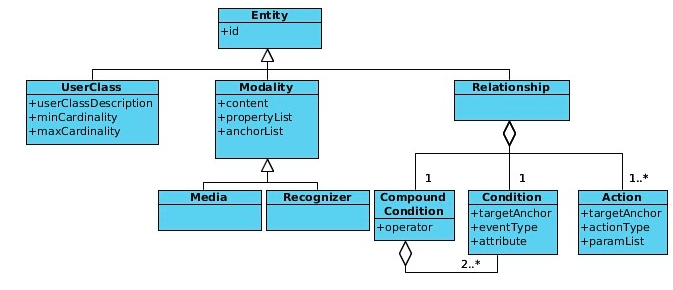
\includegraphics[width=12cm, keepaspectratio]{img/img9.png}
	\caption{Class diagram for the proposed model.}
	\captionvspace
	\label{fig:model}
\end{center}
\end{figure}

The model is based on the NCM entities~\cite{soares_nested_2009}. In particular,
we follow a structure-based~\cite{bolt_put-that-there:_1980} paradigm, which
means that the multimedia document is decoupled from the modalities contents. A
language following our model acts as glue language and does not restrict or
define what kinds of \textit{Media} and 
\textit{Recognition} are supported. \fig{fig:shematic} depicts this structure, 
in which a
multimedia document should define how \textit{Media}, \textit{Recognition}, and 
\textit{UserClass }are related in time, using Relationships, not carrying their
actual contents or descriptions. Then, if one changes the contents of an entity,
from a 
\textit{Media}, \textit{Recognizer}, or \textit{UserClass}, this will not change
the document structure. For instance, in the “Put-That-There” scenario, the
speech synthesis can be replaced by a video or the gesture recognition can be
replaced by speech recognition.

\begin{figure}[!ht]
\begin{center}
	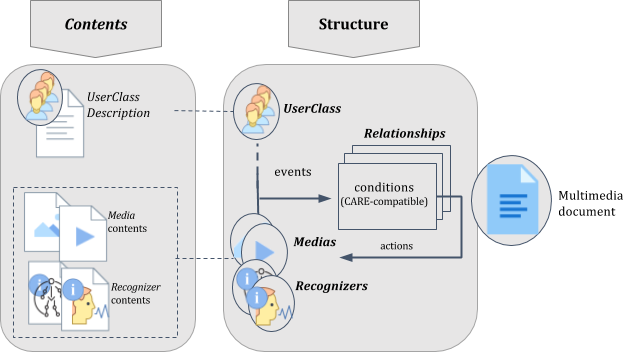
\includegraphics[width=10cm, keepaspectratio]{img/img10.png}
	\caption{Schematic view of the proposed multimedia document.}
	\label{fig:shematic}
    \captionvspace
\end{center}
\end{figure}

The next subsections detail each entity of the model.

\section{Media and Recognizer}
\label{sec:approuach:node} An interaction modality can be specialized in two
main entities: \textit{Media} and 
\textit{Recognizer}. It is defined by its Content, a list of \textit{anchor}s,
and a list of \textit{properties}.

\textit{Media} entities are capable of producing output in certain modalities
through audiovisual devices and actuators. For instance, a TTS (Text-To-Speech)
synthesizer produces audio speech to be played through a speaker. Similar to the
recognizer \textit{content}, the media \textit{content} is also decoupled from
the multimedia document and it is referenced by a location property. The media
\textit{content} can be an ordinary audiovisual content —such as audio, video,
image— or a document described in a unimodal synthesizer language, \textit{e.g.} an SSML
file. \textit{Anchor}s are portions of the content presentation. For instance,
an \textit{anchor} may define a temporal portion of a video (\textit{e.g.} a segment of
the video presentation ranging from 30 to 50 seconds). Additionally, an
\textit{Anchor} may refer to the identifier of an internal element in the
synthesizer document, \textit{e.g.} an SSML element to be synthesized. \textit{Properties}
define parameters for \textit{Media}, such as the transparency of video, the
volume of the audio output produced by an SSML speech synthesizer, the frame
rate of a BML avatar rendering animation, etc.

\textit{Recognizer} entities are capable of identifying an expected input in a
certain modality captured from an input device or sensor. For example, an ASR
(Audio Speech Recognition) recognizer identifies sentences in audio samples
captured by a microphone. The \textit{content} of a \textit{Recognizer} is
decoupled from the multimedia document and it is referenced by a location
property (the URL of the content). The content can be a document described in a
unimodal recognizer language, \textit{e.g.} an SRGS file. \textit{anchor}s are portions
of the recognizer content. They define when or what to expect, within a
document, a certain input modality to be recognized. For instance, an SRGS
defines one rule element for each expected speech input (\textit{e.g.} a certain rule may
define that acceptable input tokens are “put that” and “there”). An anchor
enables the multimedia document to know the moment when the recognition of a
token is complete. \textit{Propertie}s define parameters for the
\textit{Recognizer} or dynamic values inside the \textit{Recognizer}. For
example, an ink recognizer can have properties to indicate the current position
of the ink pointer. 

\section{UserClass}
\label{sec:approuach:userclass}

In multiuser applications, a user may assume different roles. For instance, it
is possible to create an application that behaves differently if the user is a
professor or a student. Moreover, both professors and students can use the
application at the same time. By supporting multiuser features in the authoring
model, a developer can create applications that are aware of the users who are
interacting with them, and how. To support multiuser features, the 
\textit{UserClass} is used to model the different types of interacting users,
\textit{i.e.}~different roles that users can play when using an application.

A \textit{UserClass} is defined by its \textit{minCardinality} and 
\textit{maxCardinality} attributes, and by a \textit{userClassDescription}. The
id attribute uniquely defines a UserClass. The cardinality attributes allow us
to limit the number of users that can be part of that \textit{UserClass}. The
\textit{userClassDescription} specifies how users are identified as being part
of the \textit{UserClass}. To do that, each user who can interact with the
system must have a \textit{profile description}. The user profile may include,
for example, information such as whether he/she is a student or a professor.
Moreover, it may include the devices he/she is using to interact with the
application. The \textit{userClassDescription} then should specify which users,
based on their profiles, are part of each \textit{UserClass}. 

Note that the specification of \textit{userClassDescription} is tied to the
specific vocabulary used to describe the user’s profiles. Our model is agnostic
and does not prescribe the \textit{userClassDescription} specification details,
which should be defined by the language instantiation. For instance, we propose
in our language instantiations (discussed in \chp{chp:instantiation}) the use
of an RDF description for user 
\textit{profile description }and \textit{SPARQL}, which enables queries over RDF
entities, for 
\textit{userClassDescription}.

Runtime properties related to users in a \textit{UserClass}, such as the number
of users registered in a class and user context, should be stored as global
variables. In particular, regarding the user context, the language must support
the description of human sensory capabilities, which can be used during modality
selection. Examples of such variables are \textit{canHear}, \textit{canSee}, and
\textit{canSpeak}. Therefore, a modality selection can be specified through
conditional control structures, such as \textit{switch }or
\textit{if-then-else}, which evaluate these runtime properties.

\tab{table:selection} shows examples of modality selection considering users’
sensory capabilities.\footnote{The recommendation of modalities given users’
sensory capabilities should draw on accessibility research results. 
\tab{table:selection} is simply an illustration that our approach makes it
feasible to build MUIs considering those capabilities.} For instance, when the
\textit{canSee} variable is 
\textit{false}, audio or speech modalities should be used instead of visual and
GUI modalities; and when \textit{canHear} is \textit{false} an avatar-based
modality should be selected instead of audio modalities.

\begin{table}
\setlist[itemize]{topsep=0pt}
\scriptsize
\def\arraystretch{1.5}
\begin{tabular}[!ht]{ c m{5.5cm} m{5.5cm}}

	\hline
	\textbf{Variables} & 
	\centering\arraybackslash \textbf{When false} & 
	\centering\arraybackslash \textbf{When true} \\
	\hline

	canSee &	
	\begin{itemize}
		\item Audio modalities \newline (\textit{e.g.} audio/*)
		\item Speech modalities \newline (\textit{e.g.} SRGS, SSML)
	\end{itemize}
	&	
	\begin{itemize}
		\item Visual modalities (\textit{e.g.} \newline video/* img/*, text/plain) 
		\item GUI modalities (\textit{e.g.} key presses, mouse
	\end{itemize} \\
	\hline
	
	canHear &
	\begin{itemize}
		\item Avatar modalities \newline (\textit{e.g.} BML)
	\end{itemize} 
	&		
	\begin{itemize}
		\item Audio modalities \newline (\textit{e.g.} audio/*)
	\end{itemize}\\
	\hline
	
	canSpeak &	
	\begin{itemize}
		\item Audio modalities \newline (\textit{e.g.} audio/*)
	\end{itemize}
	&	
	\begin{itemize}
		\item Speech modalities \newline (\textit{e.g.} SRGS, SSML)
	\end{itemize}\\
	\hline

\end{tabular}
\caption{Examples of modality selection.}
\label{table:selection}
\end{table}

This thesis focuses on specification issues of multiuser interactions. More
precisely, we focus on how the author defines user interaction requirements and
uses context information. We do not directly address, nor prescribe, how the
multimedia system should gather the users’ \textit{profile description} and
retrieval of their runtime context variables. These tasks can be achieved by
explicit user identification (\textit{e.g.} via log in) or by recognition techniques using
sensors (\textit{e.g.} via facial recognition).

\section{Relationship}
\label{sec:approuach:relationship}

\textit{Relationship} entities enable developers to express the combined use of
the modalities perceived by users through \textit{Media} and the modalities
generated by users through \textit{Recognizers}. In the “Put-That-There”
scenario, for instance, Relationship entities express the combined use of speech
syntheses and visual objects (\textit{Media}) with the speech and gesture
recognition (\textit{Recognizers}). 
\textit{Relationship} entities are defined by a set of \textit{conditions} and 
\textit{actions}. When the 
\textit{conditions} are satisfied, then the \textit{actions} are performed. The
actions and 
\textit{conditions} in a \textit{Relationship} are detailed as follows. 

Regarding the \textit{actions} of the \textit{Relationship}, they enable
developers to change the properties and to control the activation/deactivation
of \textit{Recognizers} and \textit{Medias}. A \textit{set} action changes the
value of a property. Four actions can manipulate the activation/deactivation of
\textit{Recognizers} and \textit{Media}: \textit{start}, which activates a
recognizer or synthesizer; \textit{stop}, which deactivates a
\textit{Recognizer} or \textit{Media} and releases its resources;
\textit{pause}, which deactivates a \textit{Recognizer} or \textit{Media}, but
does not release its resources; and \textit{resume}, which reactivates a
previously paused \textit{Recognizer} or \textit{Media}.
\tab{table:relationship} presents the semantics of those actions over
\textit{Recognizers}, \textit{Media}, and their \textit{anchors}.

In a \textit{Recognizer}, the activation of an anchor “a1” means that the
portion of the 
\textit{Recognizer} content related to “a1” is enabled to be recognized. By
default, activating a \textit{Recognizer} without specifying a specific
\textit{anchor} is equivalent to activating all of its \textit{anchor}s. The
recognition of the \textit{anchor} content itself only occurs when the
\textit{Recognizer} identifies the required pattern in the user input in the
corresponding modality. For instance, consider a speech recognizer that defines
two anchors, for the tokens “put that” and “there”. When the recognizer is
activated without specifying an anchor, both anchors are activated and, thus,
either one can be recognized in the audio input (\textit{e.g.} captured by a 
microphone).
Moreover, the developer can restrict the recognizable content by starting the
anchors individually.

\begin{table}[H]
\scriptsize
\def\arraystretch{1.5}
\begin{tabular}[!ht]{ m{1cm} m{4.5cm} m{7cm} }
	%%%%%% 
	\hline
	\textbf{Action} & \textbf{Over}
		& \textbf{Semantics} \\

	%%%%%% 
	\hline
	\multirow{7}{*}{start} 
	& \textit{Media} &\textit{Media} starts rendering its content from the beginning.\\
	\cline{2-3}
	& An anchor of a \textit{Media} &	\textit{Media} starts rendering its
	content from that specific anchor. \\
	\cline{2-3}
	& \textit{Recognizer} &	\textit{Recognizer} is activated and it is able to 
	recognize all of the anchors of the recognizer content. \\
	\cline{2-3}
	& An anchor of a \textit{Recognizer} &	\textit{Recognizer} is activated 
	and it is able to recognize only the content related to that specific 
	anchor. \\
	\hline

	%%%%%% 
	\multirow{6}{*}{stop}
	& \textit{Media} & \textit{Media} stops rendering its content.\\
	\cline{2-3}
	& An anchor of a \textit{Media} &	\textit{Media} stops rendering the 
	content of that specific anchor. \\
	\cline{2-3}
	& \textit{Recognizer} &	\textit{Recognizer} is deactivated and it is unable 
	to recognize any content. \\
	\cline{2-3}
	& An anchor of a \textit{Recognizer} &	\textit{Recognizer} is deactivated 
	and it is unable to recognize the content related to that specific anchor.\\
	\hline

	%%%%%% 
	\multirow{5}{*}{pause}
	& \textit{Media} &	\textit{Media} pauses rendering/synthesizing its 
	content, but 
	the system does not release its resources.\\
	\cline{2-3}
	& An anchor of a \textit{Media} &	\textit{Media} pauses 
	rendering/synthesizing its 
	content from that specific anchor, but the system does not release the 
	synthesizer’s resources. \\
	\cline{2-3}
	& \textit{Recognizer} / anchor of a \textit{Recognizer} &	Acts as stop. \\
	\hline

	%%%%%% 
	\multirow{5}{*}{resume}
	& \textit{Media} &	\textit{Media} restarts rendering/synthesizing its 
	content from 
	the previously paused state. \\
	\cline{2-3}
	& \textit{Recognizer} &	\textit{Media} restarts rendering/synthesizing its 
	content 
	from the previously paused anchor. \\
	\cline{2-3}
	& \textit{Recognizer} / anchor of a \textit{Recognizer} &	Acts as start. \\
	\hline
\end{tabular}
%}
\caption{Semantics of the actions over media, recognizers, and their anchors.}
\label{table:relationship}
\end{table}

In a \textit{Media}, the activation of an anchor means that the \textit{Media}
is rendering the content related to that \textit{anchor}. While a synthesizer is
activated and being rendered, its anchors are automatically
activated/deactivated as the presentation content of the \textit{Media} reaches
the content portion related to each 
\textit{Anchor}. For instance, consider an \textit{anchor} “a1” of an
audiovisual media “m1” from 300 to 360 seconds. This \textit{Anchor} will be
automatically activated when the presentation of “m1” reaches 300 seconds, and
deactivated when it reaches 360 seconds. This behavior is similar to other types
of \textit{Media}. For instance, consider an \textit{anchor} “a2” that points to
a specific token of an SSML document associated to \textit{Media} “s1”. In 
this case, when the presentation of the SMML document —\textit{i.e.}~the speech 
synthesis— reaches the token related to “a2”, then “a2” is activated.

A \textit{condition} may test:

\begin{itemize}	
	\item the activation of \textit{Recognizers} and \textit{Media}, or their
	anchors. For instance, we can define a \textit{Relationship} to be triggered
	when a (portion of a) video is activated with given attributes;
	\item the recognition of portions of the \textit{Recognizer} content. For
	instance, we can define a \textit{Relationship} to be triggered when the
	recognition of “hello”, defined in an SRGS file, is complete;
	\item values of properties of \textit{Recognizer} or \textit{Media} and
	runtime of a user’s context. For these value tests, the multimedia language
	must provide comparators, such as: is equal to, greater than, and less than.
	For instance, we can define a Relationship to be triggered when the volume of a video becomes greater than 70\% or when the \textit{canHear} value is equal to “false”.
\end{itemize}	

\textit{CompoundCondition}s specify the combined use of \textit{conditions} over
the modalities. For instance, a \textit{Relationship} can be defined to be
triggered when portions of a video are activated and the recognition of a
sentence is complete. The following operators are proposed here:

\begin{itemize}	
	\item \textit{or}: the \textit{Relationship} will trigger when any one of the
	conditions is satisfied;
	\item \textit{and}: the \textit{Relationship} will trigger when all the
	conditions are satisfied, independently of the order in which they are
	satisfied; 
	\item \textit{seq}: the \textit{Relationship} will trigger when all the
	conditions are satisfied in the specified order. This operator was not present in the relationship entity of NCM.
\end{itemize}	

\begin{table}[b!]
\scriptsize
\def\arraystretch{1.3}
\begin{tabular}{ m{4cm} m{4.5cm} m{4.5cm}}
	%%%%%% 
	\hline
	\textbf{CARE properties} & \textbf{Relationship operators \newline (our approach)} & \textbf{SMUIML transition operators} \\
	\hline
	
	%%%%%% 
	\textbf{Equivalence} &	Compound condition using the or operator &	
	Recognizers 
	trigger using the seq\_or operator \\
	\hline
	\textbf{Assignment} &	A simple condition &	Only one trigger \\
	\hline
	\textbf{Redundancy (use temporal window)} & Compound condition using the or 
	operator 
	and activated within a temporal window &	Recognizers trigger using the 
	par\_or operator \\
	\hline
	\textbf{Sequential complementarity} & Compound condition using the seq 
	operator &	
	Recognizers trigger using the seq\_and operator \\
	\hline
	\textbf{Parallel complementarity (use temporal window)} & Compound 
	condition using 
	the and operator and activated within a temporal window &	Recognizers 
	trigger using the par\_and operator \\ 
	\hline

\end{tabular}
\caption{Expressiveness of the multimodal \textit{Relationship} operators 
compared to 
SMUIML.}
\label{table:care}
\end{table}

Indeed, the combination of interaction modalities is an important feature of
MUIs. To analyze the expressiveness of the proposed operators, 
\tab{table:care} compares them to the CARE properties. \textit{Equivalence} can
be expressed by a compound condition using the or operator. \textit{Assignment}
can be expressed by a simple condition. \textit{Redundancy} can be expressed by
compound conditions using the \textit{or} operator defined within a temporal
window. The temporal window may be defined by activating/deactivating modalities
within a specific period of time. 
\textit{Sequential complementarity} is expressed by a compound condition using
the \textit{seq} operator. Finally, \textit{parallel complementarity} is
expressed by a compound condition using the \textit{and} operator defined within
a temporal window. As highlighted in \tab{table:care}, the proposed operators
have the same expressiveness as the CARE properties and SMUIML operators.
However, CARE properties and SMUIML operators consider only input modalities,
whereas our approach supports simple and compound conditions relating any
combination of input and output modalities. In addition, our proposal supports
conditions for evaluating the user’s context.

To support multiuser-oriented development, the recognition \textit{condition} in
a \textit{Relationship} can be parameterized with a “user\_id” attribute. The
value of this attribute defines which specific user from a \textit{UserClass}
can be responsible for generating the event. By doing this, it is possible to
limit which specific users can trigger a \textit{Relationship}. Moreover, we
define another optional attribute in conditions, called “excluded\_user\_id”. In this attribute, developers can define a list of users who are not allowed to
trigger a condition.

\section{Discussion}
\label{sec:approuch:discussion}

We argue in this thesis, that an multimedia language that instate our entities will support both multimodal and multiuser interactions. We believe that these extensions can contribute to the state of the art by overcoming the drawbacks and same time increase multimodal specification expressiveness.

We handled the lack of support for fine synchronization among modalities mainly
by reusing the multimedia players’ infrastructure, which keeps media object
presentations finely synchronized. In our approach, the multimedia language and
its player should also handle recognizers for input events, in the same
infrastructure. The recognizers are responsible for interacting with the user
input devices and sensors, and for triggering anchor events that enable
synchronization by the multimedia player.

Regarding the strong encapsulation between fusion and fission, we solved this
issue by using a structure-based~\cite{bulterman_structured_2005} paradigm and
using the NCM anchor concept. In addition, we have extended this concept to be
used not only by output modalities (\textit{e.g.} instantiated as <media> in NCL), but
also by input modalities (<input>). By so doing, the multimedia document is
decoupled from the content for recognizers and synthesizers. If necessary,
however, the internal behavior of those recognizers and synthesizers can be
known and controlled by the multimedia application through their anchor events.
Conversely, the languages and frameworks discussed in \chp{chp:approach} 
delegate one of
them to another entity. For instance, SMUIML sends ad-hoc messages to a
HephaticsTK framework client. 

To solve the lack of support for modality selection considering sensory
capabilities, the framework uses context variables that are able to express user
capabilities. Those variables could be used in conditional constructions to
enable the right modality selection based on the user’s sensory capabilities.

Finally, we overcame the interacting users are second-class citizens through
enabling the specification of interacting users, and the association of a user
with recognition events.

Besides overcoming the above drawbacks, our proposal also achieves more
expressiveness when combining both output and input modalities. It does so by
using the causal relationship and anchor concepts from NCM. Those concepts
enable NCM express Allen’s temporal relations among output modalities. In our
approach, we enable such concepts for input modalities which enable it express
Allen’s temporal relations among both output modalities and input modalities.

%%%%%%%%%%%%%%%%%%%%%%%%%%%%%%%%%%%%%%%%%%%%%%%%%%%%%%%%%%%%%%%%%%%%%%%%%%%%%%%%
\chapter{Language instantiations}
%%%%%%%%%%%%%%%%%%%%%%%%%%%%%%%%%%%%%%%%%%%%%%%%%%%%%%%%%%%%%%%%%%%%%%%%%%%%%%%%
\label{chp:instantiation}

The model presented in the previous chapter was proposed to be agnostic to 
multimedia languages and their syntax. In this section, we discuss the 
instantiation of the model entities as first-class citizens and their proposed 
syntax in two multimedia languages: NCL (\sect{sec:ncl}) and 
HTML (\sect{sec:html}).

\section{NCL instantiation}
\label{sec:ncl}

NCL 3.0 is an XML multimedia language based on the Nested Context Model (NCM)
3.0, a model for hypermedia document specification which allows defining
temporal and spatial relationships among media objects. The current entities of
NCM 3.0 do not focus on representing either modalities different from the
GUI-based ones, or interactions aware of the users who interact with the
application. To overcome these limitations, we first instantiate our entities in
NCM 3.0. \fig{fig:ncm}\footnote{Some NCM entities are omitted from the 
discussion here for simplicity (e.g. Descriptor, SwitchPort) or because they 
are not used in NCL 3.0 (\textit{e.g.} ConstraintConnector). For a complete 
description of NCM, we refer the reader to \cite{soares_nested_2009}} 
illustrates the current NCM entities, highlighted in light blue, and our 
extensions, highlighted in light green. \appen{annex:schemas} presents XML 
schemas, which detail our NCL 3.0 syntax extensions.

The main entities of NCM 3.0 are \textit{Node} and \textit{Link}. We briefly
detail them in what follows. 

An NCM 3.0 \textit{Node} is defined by its content, a descriptor, and a list of
anchors. 
\textit{Content} is the collection of information of a node. Descriptor defines
properties for how a node should be exhibited, such as position for graphics,
frame rate for video, and volume for audio. The \textit{Anchor}s in the list of 
\textit{Anchor}s
can be of two types: \textit{ContentAnchor}, which represents portions of the
content of the node; or \textit{AttributeAnchor}, which represents a property of
the node. 
\textit{ContentNode} and \textit{CompositeNode} are specializations of Node and
detail the semantics of Content and \textit{ContentAnchor}. \textit{ContentNode}
has been specialized mainly for 2D audiovisual media modalities, such as
\textit{TextNode}, \textit{ImageNode}, and \textit{VideoNode}. 
\textit{ContentAnchor}s of \textit{ContentNode} are spatial or temporal 
portions of the corresponding media objects. For instance, the \textit{Content} 
of a \textit{VideoNode} may be defined via references to a video file 
(\textit{e.g.} file URI) and its temporal anchors by references to 
its presentation times.

An NCM \textit{Link} is defined by a \textit{Connector} and a list of 
\textit{Bind}s. 
\textit{Connectors} define the link semantics, independently of the 
participating \textit{Node}s.
More precisely, a \textit{Connector} defines the relation between 
\textit{Role}s and not between specific \textit{Node}s. When instantiating a 
\textit{Connector}, one \textit{Link} must define the association 
(\textit{i.e.}~\textit{Bind}) of each connector \textit{Role} to 
a node interface (\textit{ContentAnchor}, \textit{AttributeAnchor} or 
\textit{Port}s).

A Role is defined by the attributes: \textit{RoleID}, \textit{EventType}, 
\textit{minCardinality}, and 
\textit{maxCardinality}. The \textit{EventType} refers to a specific event
related to an \textit{Anchor}. NCM 3.0 has three main event types:
\textit{PresentationEvent}, meaning the exhibition of a \textit{ContentAnchor};
\textit{AttributionEvent}, meaning the modification of a node property
(\textit{AttributeAnchor}); and \textit{SelectionEvent}, meaning a mouse click
or key-based event while a specific \textit{ContentAnchor} is occurring. In
particular, the \textit{SelectionEvent} has a key attribute that defines the 
key (\textit{e.g.} keyboard or remote control) that triggers the event.

Whereas a connector may represent any kind of relationship between node anchors,
NCL 3.0 defines only the \textit{CausalConnector} relationship. 
\textit{CausalConnector} specifies which conditions (\textit{ConditionRoles})
need to be satisfied to trigger actions (\textit{ActionRoles}). A
\textit{ConditionRole} can be a \textit{SimpleCondition} or a
\textit{CompoundCondition}. \textit{SimpleCondition}s act over \textit{Node}s 
and may test the occurrence of an event (\textit{e.g.} when the event state 
changes to “occurring”). \textit{CompoundCondition}s represent a logical 
expression using “and” or “or” operators through \textit{SimpleCondition}s and
\textit{AssessmentSatement}s. An \textit{AssessmentSatement} is used to compare 
event attributes. For instance, \textit{SelectionEvent} has a key attribute, 
which can be tested in \textit{SimpleCondition} or 
\textit{AttributeAssessment}. Finally, \textit{ActionRole} may define changes 
in presentation state or properties of \textit{Node}s.

In the remainder of this section (subsections \ref{sec:instantiation:node} 
and \ref{sec:instantiations:link}), we present our extensions to NCM and NCL 
aiming to address these limitations.

\begin{landscape}
\begin{figure}
	\begin{center}
		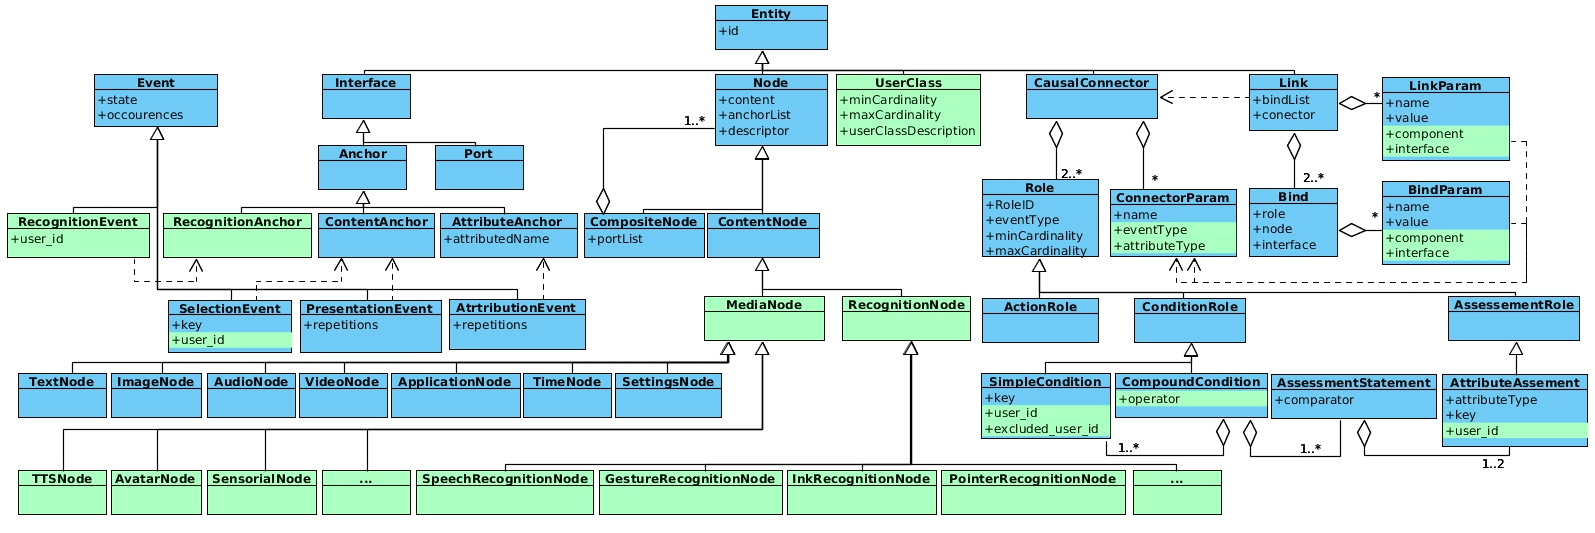
\includegraphics[height=8cm, keepaspectratio]{img/img11.png}
		\caption{NCM 3.0 and proposed extensions.}
		\label{fig:ncm}
	\end{center}
\end{figure}
\end{landscape}

\subsection{Multimodal specializations for Node}
\label{sec:instantiation:node}

To add our \textit{Media} and \textit{Recognizer} entities to NCM 3.0, we 
propose multimodal 
specializations for Node, named \textit{MediaNode} and \textit{RecognitionNode}.

In a \textit{ContentNode} of NCM 3.0, we group the audiovisual modalities as 
specializations of the new \textit{MediaNode} class, which is itself a 
specialization of 
\textit{ContentNode}. Also, we propose three new \textit{MediaNode} 
specializations for 
representing output modalities: (1) \textit{TTSNode}, representing a TTS 
(Text-To-Speech) content (as described in W3C 
SSML~\cite{daniel_c._burnett_speech_2010}, for example), useful 
for visually impaired users; (2) \textit{AvatarNode}, representing embodied 
conversational agents (\textit{e.g.} described using BML~\cite{vilhjalmsson_behavior_2007}), useful for deaf-, 
children- or elderly-oriented interfaces; and (3) \textit{SensorialNode}, 
representing 
sensorial effects (\textit{e.g.} described in MPEG-V SEDL~\cite{iso/iec_iso/iec_2013}), useful for increasing 
the QoE~(Quality of Experience)~\cite{ghinea_mulsemedia:_2014} of multimedia presentations. Other 
specializations to \textit{MediaNode} 
representing other modalities can be seamlessly integrated in the future.

For the representation of input modalities, we propose the new 
\textit{RecognitionNode} 
as a specialization of \textit{ContentNode}, which can be used in Link 
elements. The Content of a \textit{RecognitionNode} is also a collection of 
information. Different from the \textit{MediaNode}, however, the information is 
expected to be captured, not presented. Some examples of 
\textit{RecognitionNode} specializations include: (1) 
\textit{SpeechRecognitionNode}, used for speech recognition, such as 
recognizing words 
and phrases spoken by the user(s); (2) \textit{GestureRecognitionNode}, used 
for gesture 
recognitions; (3) \textit{InkRecognitionNode}, used for pen writing (“ink”) 
recognitions; (4) \textit{PointerRecognitionNode}, used for recognizing 
interaction from 
a pointer device; and (5) \textit{KeyRecognitionNode}, used for recognizing 
interactions 
from keyboard devices. Some examples of how the Content of those nodes may be 
represented include: W3C SRGS~\cite{andrew_hunt_speech_2004} for \textit{SpeechRecognitionNode}; GDL 
(Gesture 
Description Language)~\cite{hachaj_semantic_2012} for 
\textit{GestureRecognitionNode}; and InkXML~\cite{w3c_ink_2011} for 
\textit{InkRecognitionNode}. Also, other specializations to 
\textit{RecognitionNode} representing 
other input modalities can be seamlessly integrated in the future.

Since \textit{RecognitionNode} is indeed a specialization of 
\textit{ContentNode}, it is also 
possible to define Anchors in it. A special type of Anchor, the 
\textit{RecognitionAnchor}, specifies a portion of the recognition content and 
is 
associated to a “recognition” event. For instance, a \textit{RecognitionAnchor} 
may refer to expected speech tokens defined in a \textit{SpeechRecognitionNode} 
or 
a “move” or “click” anchor to a \textit{PointerRecognitionNode}. The 
“recognition” event indicates that the system has recognized the expected 
information defined in a \textit{RecognitionAnchor}. It is important to 
highlight that the occurrence of events issued by a \textit{RecognitionNode} is 
not intrinsically coupled with \textit{MediaNode} events. 

Based on the above extensions to the NCM, we also defined how those changes 
can be mapped onto NCL 3.0, the concrete syntax of the model.

NCL 3.0~\cite{abnt_abnt_2016} defines the <media> element for 
specifying audiovisual media in a 
multimedia document. It has the advantage of being media-type agnostic. 
Following the same principle, we propose to use <media> elements to support not 
only audiovisual media, but also any type of synthesized description, such as 
SSML and SEDL. Therefore, there are no changes in the <media> element.

To allow the integration of \textit{Recognizer} in NCL, we propose a new 
element for the 
language, named <input>, because NCL 3.0 only considers GUI-based interactions. 
Analogous to <media>, <input> defines the \textit{Recognizer} content location 
(src), 
its properties (<property>), and its anchors (<area>). The src attribute refers 
to the Recognizer content, described in languages such as SRGS and GestureML. 
To represent that a content was recognized, we define a new event type, 
named “recognition” event, which can only be associated to <input> elements. 
Similar to other types of events, it introduces reserved words for the start of 
the recognition (“onBeginRecognition”) and for its end (“onEndRecognition” or 
“onRecognize”). 

To illustrate the usage of the these multimodal specializations, we created an 
extended version of “Sightseeing of Today”~\cite{fernando_o_2009}, an 
interactive non-linear video~\cite{meixner_interactive_2012} about sightseeing 
in a city. In its original version, the user interacts 
via key/mouse to navigate between videos; in some opportunity time windows, the 
user can choose which touristic place the user will be guided next. The choice 
is: if the user presses the RED button, the “downtown” video is started; and if 
the user presses the GREEN button, then the “beach” video is started. Our 
extended version, named “Multimodal Sightseeing of Today”, enables video 
navigation also via voice commands.

“Multimodal Sightseeing of Today” uses two multimodal descriptions, an SSML 
(\lis{list:ssml}) and an SRGS (\lis{list:srgs}) file, to enable the user to 
choose which video to play next. 

\lis{list:ncl-sightseeing} shows the code fragment responsible for controlling 
the first 
navigation. It defines four <media> and one <input> elements. Three <media> 
elements (“intro”, “videoDowntown” and “videoBeach”, lines 16-25) define the 
introductory video and the two videos available for the user to choose from. 
The “intro” video has an anchor (“choice\_moment”) starting at 40 seconds in 
the 
video. The fourth <media> “audio\_choice” (lines 26) refers to speech synthesis 
and the “asr\_places” <input> (lines 27-30) supports voice commands for 
navigation control in this first interaction opportunity. This <input> element 
defines two anchors mapping onto rules specified in the “places.sgrs” file, 
defining the words “downtown” and “beach”.

Regarding the application behavior, it begins by starting the “intro” video 
(line 15) and defines three <link> elements. The first link (lines 31-36) 
defines that, when the “choice\_moment” anchor is reached, then application 
asks 
for possible places via voice command. The other two links (lines 37-44) define 
that when the user says the name of a recognized place, then the corresponding 
video should be started.

\begin{listing}[!ht]
\begin{minted}[linenos,fontsize=\scriptsize,numbersep=1pt,frame=lines,xleftmargin=10pt,framesep=2mm]{xml}
<speak xmlns="http://www.w3.org/2001/10/synthesis">
  <s>Do you want visit the Rio de Janeiro’s downtown or the 
  Copacabana beach?</s>
  ...
</speak>
\end{minted}
\caption{downtown\_or\_beach\_audio.ssml.}
\label{list:ssml}
\end{listing}

\begin{listing}[!ht]
\begin{minted}[linenos,fontsize=\scriptsize,numbersep=1pt,frame=lines,xleftmargin=10pt,framesep=2mm]{xml}
<grammar xmlns="http://www.w3.org/2001/06/grammar">
  <rule id="downtown">downtown</rule>
  <rule id="beach">beach</rule>
  ...
</grammar>
\end{minted}
\caption{places.sgrs.}
\label{list:srgs}
\end{listing}

\begin{minted}[linenos,fontsize=\scriptsize,numbersep=1pt,frame=lines,xleftmargin=10pt,framesep=2mm]{xml}
<ncl xmlns="http://www.ncl.org.br/NCL3.0/EDTVProfile">
  <head>
    <connectorBase>
      <causalConnector id="onBeginStart">
        <simpleCondition role="onBegin"/>
        <simpleAction role="start"/>
      </causalConnector>
      <causalConnector id="onRecognizeStart">
        <simpleCondition role="onRecognize"/>
        <simpleAction role="start"/>
      </causalConnector>
    </connectorBase>
  </head>
  <body>
    <port component="intro"/>
    <media id="intro" src="intro.mp4">
      <property name="size" value="100%, 100%"/>
      <area label="choice_moment" begin="40s"/>
    </media>
    <media id="videoDowntown" src="downtown.mp4">
      <property name="size" value="100%, 100%"/>
    </media>
    <media id="videoBeach" src="beach.mp4">
      <property name="size" value="100%, 100%"/>
    </media>
    <media id="audio_choice" src="audio_downtown_or_beach.ssml"/>
    <input id="asr_places" src="places.sgrs">
      <area label="downtown" />
      <area label="beach" />
    </input>
    <link xconnector="onBeginStart">
      <bind role="onBegin" component="intro" interface="choice_moment"/>
      <bind role="start" component="audio_choice"/>
      <bind role="start" component="asr_places" interface="downtown" />
      <bind role="start" component="asr_places" interface="beach"/>
    </link>
    <link xconnector="onRecognizeStart">
      <bind role="onRecognize" component="asr_places" interface="beach"/>
      <bind role="start" component="videoBeach"/>
    </link>
    <link xconnector="onRecognizeStart">
      <bind role="onRecognize" component="asr_places" interface="downtown"/>
      <bind role="start" component="videoDowntown"/>
    </link>
    ...
  </body>
</ncl>
\end{minted}
\begin{listing}[!ht]
\caption{“Multimodal Sightseeing of Today” NCL application.}
\label{list:ncl-sightseeing}
\end{listing}

\subsection{Linking Multiple Modalities and Users}
\label{sec:instantiations:link}

An important feature of MUIs is the combination of interaction modalities.
According to Nigay and Coutaz~\cite{coutaz_four_1995}, this combination can be:
redundant, when only one of the interactions is needed; complementary, when all
interactions are needed; or sequentially complementary, when all interactions
are needed in a specific order. To support these combinations in NCL, authors
may use \textit{CompoundCondition}s with \textit{RecognitionNode}s. Using the
“or” operator, authors can define alternative (redundant) ways in which the user
may interact. Using the “and” operator authors can define complementary
interactions. In addition to the operators already defined by NCM, we include a
new “seq” operator, through which authors can define a required sequence of
interactions. In the “Put-That-There” scenario, for instance, authors must use a
“seq” operator to guarantee that the interactions must occur in the specified
order (first, the “put that”; then, the “logo” selection, etc.).

To enable multiuser features in NCM, we created a new \textit{UserClass} entity.
In NCL 3.03 syntax, we add the <userClass> element defined inside <userBase>, in
the document head (<head> element). It has id, min, max, and
userClassDescription attributes. The userClassDescription is a URL to an
external document describing the UserClass. As previously mentioned,
userClassDescription is tied to how user profiles are specified. 

In our proposed instantiation, the system identifies the user and defines their
profiles in RDF (Resource Description Framework)~\cite{w3c_rdf/xml_2014}. Then a \textit{userClassDescription} can use a SPARQL~\cite{w3c_sparql_2008} query to
choose among the users. Each user is a foaf:Person element from the
FOAF~\cite{brickley_foaf_2014} RDF vocabulary, used for user profiles.
Additionally, this foaf:Person may define prf:name elements from
UAProf~\cite{openmobilealliance_wag_2001} RDF vocabulary, used to define device
profiles. The SPARQL query is responsible for selecting which users should be
part of the \textit{UserClass}.

Once having defined a \textit{UserClass}, the developer may define
<simpleCondition> elements using an event attribute named “user\_id”, using the
scheme “user-class-id(user-id)”. For instance, a <simpleCondition> with role and
user\_id attributes with values “onRecognize” and “BoltLikeUser(1)”,
respectively, is trigged only when an interaction is recognized from the first
registered user from the “BoltLikeUser” \textit{UserClass}. Moreover, we define
another optional attribute in <simpleCondition>, called “excluded\_user\_id”. In
this attribute, authors can define the users who are not allowed to trigger a
<simpleCondition>. Such specification of user as parameter is similar to how
Soares~\cite{soares_nested_2009} uses the “key” attribute to define which key
from “selection” events may trigger a link. Indeed, the “user\_id” attribute is
defined for both “selection” and “recognition” events. As in the “key” case, the
“user\_id” attribute may also be tested by developers, in <simpleCondition>
elements. 

In our model, the \textit{UserClass} should enable access of runtime properties
related to its users. In the extended NCL, this access occurs though an <media>
element from type “x-ncl-settings” using the scheme: “user-class-id(user-id).
property-name”. For instance, the value “BoltLikeUser(1).canHear” access the
hearing capability of the first registered user from the “BoltLikeUser”
<userClass>.

Finally, it is also interesting to give authors access to the event attributes
through Links. For instance, the author can store the last “user\_id” from a
“recognition” event or the coordinates of a pointer interaction. To do that, we
defined extensions to \textit{ConnectorParam}, \textit{BindParam}, and 
\textit{LinkParam}. Besides an arbitrary string value, \textit{ConnectorParam}
can now receive an 
\textit{Interface} as well. To define that a \textit{ConnectorParam} should
receive an \textit{Interface}, we propose the 
\textit{eventType} and \textit{attributeType} attributes, which are analogous to
those of 
\textit{AttributeAssessment}. \textit{BindParam} and \textit{LinkParam} can pass
an Interface as a parameter to Connectors through the component and interface
attributes.

To illustrate the usage of these <link> multimodal and multiuser features,
\appen{annex:scenarios} presents the “Put-That-There” scenario in NCL and its two multiuser versions, namely: “I-Get-That-You-Put-It-There” and 
“Anyone-Get-That-Someone-Else-Put-It-There”.


\section{HTML instantiation}
\label{sec:html}

HTML~\cite{w3c_html_2014} is a markup language mainly focused on supporting
text-based interactive content, which has recently included support for audio
and video content (HTML 5.0). Like NCL, HTML does not focus on representing
modalities different from the GUI-based ones, nor about interactions aware of
the users who interact with the application. To overcome these limitations, we
have instantiated our proposed entities in HTML.

At some point, W3C has proposed that HTML should evolve into an XML-based
equivalent, namely XHTML, focusing on XML modularization. The browser vendors,
however, argue that HTML evolution should not follow this path and continue to
use their own markup\footnotemark. Nowadays, when an HTML document, either in 
markup or XML syntax, is loaded into a browser engine, it becomes an object 
tree following the Document Object Model (DOM) standard~\cite{w3c_dom4_2015}. 
The DOM API for HTML, simple called HTML DOM\footnotemark, allows programs 
(\textit{e.g.} browsers) and scripts to dynamically access and update the 
content, structure, and style of a document, regardless of its syntax 
(\textit{e.g.} HTML, XML). \fig{fig:htmldom} illustrates the current HTML DOM 
entities\footnotemark, in light blue, and our extensions, in light green. In 
particular, the main entities of HTML are \textit{Node} and 
\textit{HTMLElement}~\cite{mozilla_dom}. 

\footnotetext[2]{\url{https://www.w3.org/TR/html51/introduction.html}}
\footnotetext[3]{\url{https://www.w3schools.com/jsref/dom_obj_document.asp}}
\footnotetext{Some HTML DOM entities are omitted from the discussion here 
for simplicity (\textit{e.g.} HTMLBodyElement, HTMLCanvasElement, 
HTMLDivElement). For a complete description of HTML, we refer the reader 
to~\cite{mozilla_dom}}

\begin{figure}[h]
  \begin{center}
    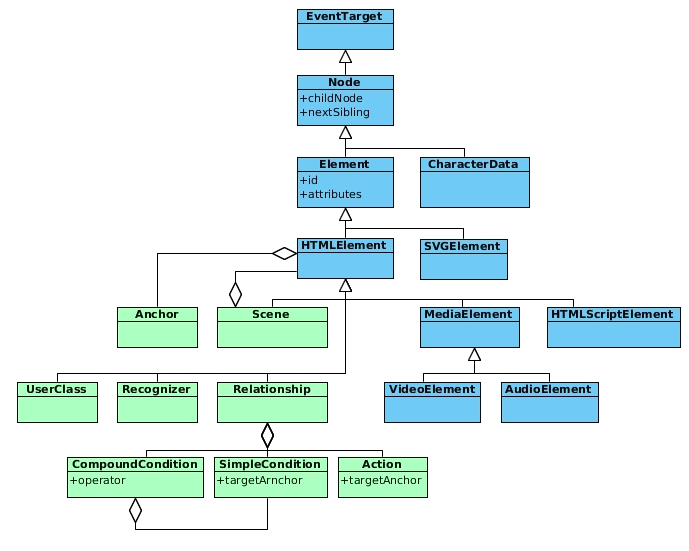
\includegraphics[width=12cm, keepaspectratio]{img/img12.png}
    \captionvspace
    \caption{HTML DOM and proposed extensions}
    \label{fig:htmldom}
    \captionvspace
  \end{center}
\end{figure}

In HTML, everything is a \textit{Node}, including the HTML document itself.
Every \textit{Node} element inherits \textit{EventTarget}, which enables the
scripts elements (HTMLScript) to use the DOM API to register event handlers on
elements in an HTML document. Nested in the HTML document node, there are both
markup elements, namely \textit{Element}, and text only nodes, namely
\textit{CharacterData}. Examples of \textit{Element} are \textit{HTMLElement}, 
for HTML markup
elements (\textit{e.g.} <div>, <img>, <p>), and 
\textit{SVGElement}, for SVG\footnotemark markup elements. Two specializations 
of \textit{HTMLElement} are \textit{HTMLScriptElement} and 
\textit{MediaElement}. The \textit{HTMLMediaElement}\footnotemark~is the basic 
entity for continuous media, such as \textit{HTMLVideoElement} and 
\textit{HTMLAudioElement}.

\footnotetext[5]{\url{https://www.w3.org/TR/SVG}}
\footnotetext[6]{\url{https://developer.mozilla.org/en-US/docs/Web/API/HTMLMediaElement}}

We propose to instantiate our entities in the HTML DOM using a browser vendor
standard called \textit{CustomElements}\footnotemark, which provides a 
JavaScript API to extend the HTML markup. In other words, it enables developers 
to create their own reusable \textit{HTMLElement}s in JavaScript. In our case, 
we propose to implement our model entities (\textit{i.e.}~\textit{Media}, 
\textit{Recognizer}, \textit{Relationship} and \textit{UserClass}) in 
JavaScript at runtime. In fact, a similar approach was followed by Soares Neto 
\textit{et al.}~\cite{neto_tal_2012}, which at preprocessing time implemented 
their template language entities (TAL) using JavaScript. 

\footnotetext[7]{\url{https://html.spec.whatwg.org/multipage/custom-elements.html\#custom-elements}}

To implement our \textit{Media} concept, we propose to reuse the existing HTML
audiovisual modalities elements, such as <img>, <audio>, <video>, and to use a
new <mm-media> element to provide synthesized modalities that inherit from
\textit{HTMLElement}. To implement the \textit{Recognizer} concept in HTML, we 
propose a new
element <mm-input>. All those elements may use a new <mm-area> to support our
ContentAnchor and RecognitionAnchor elements.

Regarding the \textit{Relationship} entity, we propose the <mm-link>. The
<mm-link> behaves like the NCL <link>, but simplified. All common connectors do
not need to be defined. Simple condition elements may be directly defined by
elements <mm-onBegin>, <mm-onEnd>, and <mm-onRecognize> and action by <mm-start>
and <mm-stop> elements. More than one condition can be grouped in a
<mm-compoundCondtion> element inside a <mm-link>. The <mm-compoundCondition>
should use an operator. 

All the proposed elements, may be grouped inside a <mm-scene> element. This
element enables the correct semantics of the <mm-link>. In HTML, <img> or
<video> elements inside the <body> are visible by default. The elements inside
an <mm-scene> are presented only be actions defined in the <mm-link> elements.

To illustrate the usage of this HTML syntax, we implemented the “Multimodal
Sightseeing of Today”. To do that, we use the same SSML (\lis{list:ssml}) and
SRGS (\lis{list:srgs}) multimodal descriptions as in the NCL version. 

\lis{list:html-sightseeing} shows the code fragment responsible for controlling
the first navigation. It defines four \textit{Media} and one <mm-input> 
element. Three \textit{Media} elements (“intro”, “videoDowntown” and 
“videoBeach”, lines 12-19) define the introductory video and the two videos 
available for the user to choose from.
The “intro” video has an anchor (“choice\_moment”) starting at 40 seconds in the
video. The fourth <mm-media> “audio\_choice” (lines 20) is speech synthesis and
“asr\_places” <mm-input> (lines 22-26) supports voice commands for navigation
control in this first interaction opportunity. This <mm-input> defines two
anchors mapping onto rules specified in the “places.sgrs” file defining the
words “downtown” and “beach”.

Regarding the application behavior, it begins by starting the “intro” video 
(line 8-11) and defines three <mm-link> elements. The first link (lines 27-32) 
define that, when the “choice\_moment” anchor is reached, then the application 
should ask for possible places via voice command. The other two <mm-links> 
(lines 33-40) define that, when the user says the name of a recognized place, 
then the corresponding video should be started.

\begin{minted}[linenos,fontsize=\scriptsize,numbersep=1pt,frame=lines,xleftmargin=10pt,framesep=2mm]{xml}
<!DOCTYPE html>
<html>
<head>
  <script src="js/elements/mm.js"></script>
</head>
<body>
  <mm-scene id="scene">
    <mm-link>
      <mm-onBegin interface="scene" />
      <mm-start interface="intro" />
    </mm-link>
    <video id="intro" src="intro.mp4" 
      style="position: absolute; height 100%; width: 100%;">
      <mm-area id="choice_moment" begin="40s" />
    </video>
    <video id="videoDowntown" src="downtown.mp4" 
      style="position: absolute; height 100%; width: 100%;">
    <video id="videoBeach" src="beach.mp4" 
      style="position: absolute; height 100%; width: 100%;">
    <mm-media id="audio_choice"
      src="audio_downtown_or_beach.ssml" />
    <mm-input id="asr_places"
      src="places.sgrs">
      <mm-area label="downtown" />
      <mm-area label="beach" />
    </mm-input>
    <mm-link>
      <mm-onBegin interface="intro.choice_moment" />
      <mm-start interface="audio_choice" />
      <mm-start interface="asr_places.downtown" />
      <mm-start interface="asr_places.beach" />
    </mm-link>
    <mm-link>
      <mm-onRecognize interface="asr_places.beach" />
      <mm-start interface="videoBeach" />
    </mm-link>
    <mm-link>
      <mm-onRecognize interface="asr_places.downtown" />
      <mm-start interface="videoDowntown" />
    </mm-link>
  </mm-scene>
</body>
</html>
\end{minted}
\begin{listing}[!hb]
\caption{“Multimodal Sightseeing of Today” HTML application.}
\label{list:html-sightseeing}
\end{listing}

Finally, we create a new <mm-userClass> with id, min, max, and 
\textit{userClassDescription} attributes. The \textit{userClassDescription} is 
a URL to a SPARQL 
document~\cite{w3c_sparql_2008} defining the required characteristics of the users. Once having 
defined an <mm-userClass>, the developer may define <mm-Selection> and 
<mm-onRecognize> elements using an event attribute named “user\_id”.

%%%%%%%%%%%%%%%%%%%%%%%%%%%%%%%%%%%%%%%%%%%%%%%%%%%%%%%%%%%%%%%%%%%%%%%%%%%%%%%%
\chapter{Evaluation}
%%%%%%%%%%%%%%%%%%%%%%%%%%%%%%%%%%%%%%%%%%%%%%%%%%%%%%%%%%%%%%%%%%%%%%%%%%%%%%%%
\label{chp:evaluation}

We address RQ1 by proposing entities (discussed in \chp{chp:approach}) to be 
instantiated
in multimedia languages. After doing so, we have also proposed syntax
instantiations for NCL and HTML (discussed in \chp{chp:instantiation}).

Nowadays, the development of NCL and HTML applications can be done using
different approaches and representations. For instance, today NCL provide
alternative representations to its XML syntax, such as JSON objects
~\cite{silva_jns:_2013} and Lua tables~\cite{moraes_lua2ncl:_2016}. Moreover, 
it is possible to develop in HTML using some alternative representations, such 
as in XML (\textit{i.e.}~XHTML) and YAML, or even to use only JavaScript to 
create the entire HTML DOM. 

Given the above context, to evaluate our answer, we confront an additional
question about \textit{“how to evaluate the usage of the proposed entities 
despite the different ways of instantiating them in a multimedia language?”}. 
In other words, if we only evaluate the usage of our proposed syntax, the 
evaluation results will be tied to the syntax development characteristics. For 
the NCL syntax, for instance, Soares Neto \textit{et 
al.}~\cite{de_salles_soares_neto_linguagens_2008}
performed a usability analysis and highlighted NCL verbosity and error-prone
characteristics. To answer such question, we performed an evaluation organized
in two parts. The first part focuses on the conceptual entities, whereas the
second part focuses on our proposed syntaxes for HTML and NCL. 

Planning the analysis for the conceptual entities was a challenge, because they
were created to be independent from representation syntax. To do so, we used a
block-based programing paradigm to enable users to develop applications using
only the concept entities, at a level of abstraction higher than that of either
NCL or HTML. This paradigm is commonly used for teaching programming or in code
generation tools. In particular, this type of development has been popularized
by tools such as MIT Scratch\footnotemark and MIT App Inventor\footnotemark. 
Although our block representation also contains its own syntax, a block syntax 
helps users to abstract away from specificities and lower-level textual syntax 
of the languages~\cite{shapiro_beyond_2016}, helping developers to focus on the 
concepts we wish to evaluate. 

\footnotetext[1]{\url{https://scratch.mit.edu/}}
\footnotetext[2]{\url{appinventor.mit.edu/}}

The analyses were performed with NCL and HTML developers through a web-based
evaluation form. This form not carry an execution runtime for the application,
i.e., the developers not visualize the multimedia application results; it focus 
only in presents model entities in the block-based and in extended language 
representations to capture their understanding and acceptance by the 
developers. In the next sections, we briefly present our block-based
representation (\subsect{sec:evaluation:blocks}), detail our evaluation form 
(\subsect{sec:evaluation:form}), and discuss the results 
(\subsect{sec:evaluation:discussion}). 

\section{Block-based representation}
\label{sec:evaluation:blocks}

Our block representation was developed using the web-based version of the
Blockly\footnotemark framework. In this framework, the blocks are defined as 
JavaScript
objects and then instantiated as SVG elements in HTML DOM. Then, those blocks as
SVG elements are showed in a workspace <div>, where the user can drag and drop
elements, fill in some fields, and join elements together. We have created four
group blocks, each one related with one entity.

\footnotetext{\url{https://developers.google.com/blockly/}}

In our block representation, a \textit{Media} entity is defined by joining a
media block, with the id field filled in, and a media content block, which can
be an image, audio, video or speech synthesis block. Similar, a Recognizer
entity is defined by joining a recognizer block, with the id field filled in,
and a recognized content block, which can be a speech or hand gesture block.
\fig{fig:blocksgroups} illustrates the block groups related with the 
\textit{Media}, 
\textit{Recognizer} and 
\textit{UserClass} entities.

\begin{figure}[!ht]
\begin{center}
	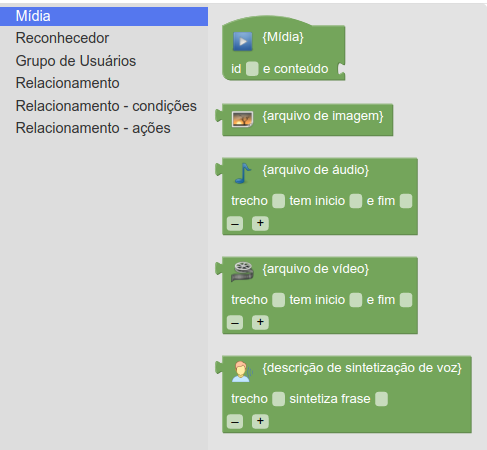
\includegraphics[width=4.4cm, keepaspectratio]{img/img13a.png}
	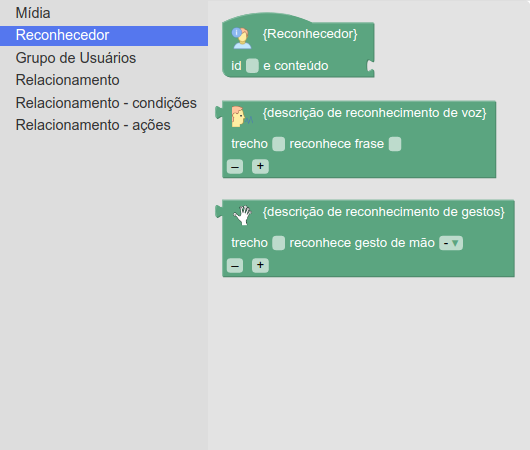
\includegraphics[width=4.4cm, keepaspectratio]{img/img13b.png}
	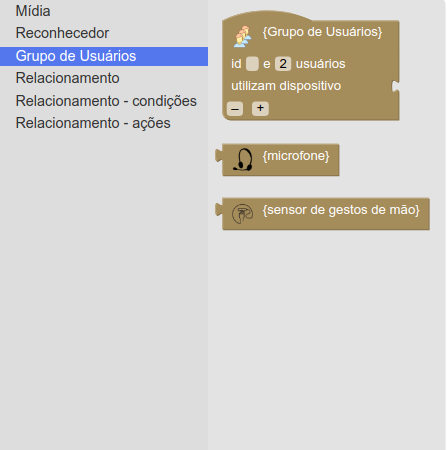
\includegraphics[width=4.4cm, keepaspectratio]{img/img13c.png}
	\caption{Blocks groups related to \textit{Media}, \textit{Recognizer} and 
	\textit{UserClass}.}
	\label{fig:blocksgroups}
	\captionvspace
\end{center}
\end{figure}

A \textit{Relationship} is defined by joining one \textit{Relationship} block
with conditions and action blocks. Condition blocks can be simple or
compound. Simple condition blocks can define the trigger for: begin or end of
media/recognizer anchor or block id; selection of media block; recognition of
recognizer anchor or block id. A compound condition block allows combining other
condition blocks and use a combination operator (“OR”, “AND”, “SEQ”). Finally,
the action blocks can be start or stop a media/recognizer anchor or block id.
\fig{fig:blocks1} illustrates the blocks related with the \textit{Relationship}
entity. To prevent users from having the fill in all id values, the fields in
these \textit{Relationship} blocks are dropdowns, which list the existing
media/recognizer anchor or block ids.

\begin{figure}[!ht]
\begin{center}
	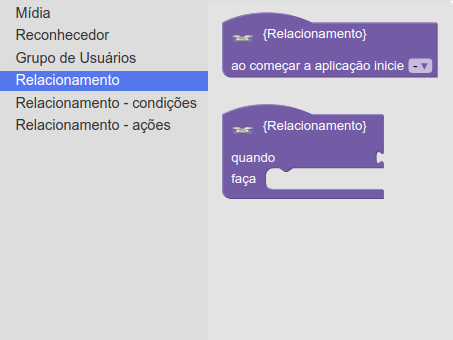
\includegraphics[width=4.4cm, keepaspectratio]{img/img14a.png}
	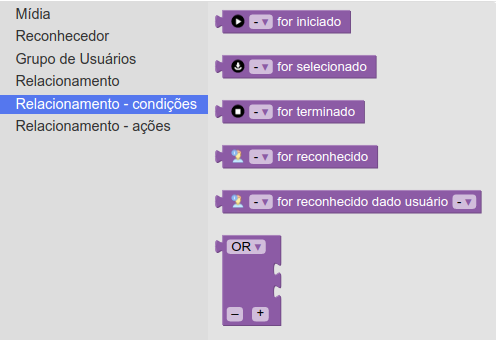
\includegraphics[width=4.4cm, keepaspectratio]{img/img14b.png}
	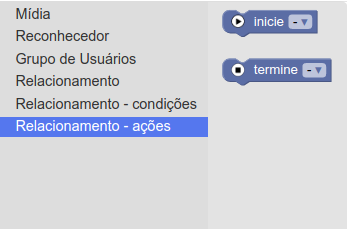
\includegraphics[width=4.4cm, keepaspectratio]{img/img14c.png}
	\caption{Blocks groups related to \textit{Relationship} related.}
	\label{fig:blocks1}
	\captionvspace
\end{center}
\end{figure}

To illustrate the usage of our block representation, \fig{fig:blocks2} presents
the “Multimodal Sightseeing of Today” application. It defines four
\textit{Media} and one 
\textit{Recognizer} (left part of \fig{fig:blocks2}). 

\begin{figure}[!ht]
  \begin{center}
    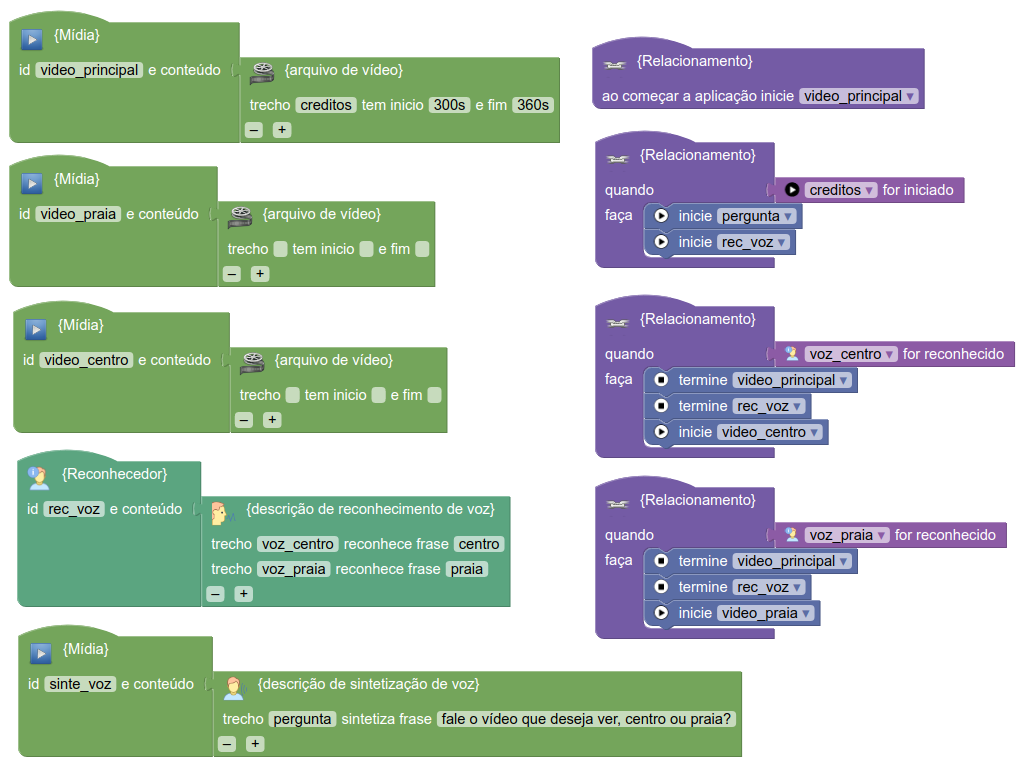
\includegraphics[width=14cm, keepaspectratio]{img/img15.png}
    \captionvspace
    \caption{Block-based representation of “Multimodal Sightseeing of Today”.}
    \captionvspace
    \label{fig:blocks2}
  \end{center}
\end{figure}

The first three \textit{Media} elements (“video\_principal”, “video\_praia” and 
“video\_centro”) define the introductory video and the two videos available for 
the user to choose from. The
“intro” video has an anchor (“creditos”) starting at 300 seconds in the video.
The last \textit{Media} (“sinte\_voz”) defines a speech synthesis media asking about the
navigation control. Finally, the \textit{Recognizer} (“asr\_places”) defines the
speech recognition for navigation control. This \textit{Recognizer} defines two 
anchors, mapping onto the words “centro” and “praia”.

Regarding the application behavior, we define four \textit{Relationship}s (right
part of the \fig{fig:blocks2}): The first one defines that the application
begins by starting the “video\_principal” video. The second one defines that,
when the “creditos” anchor is reached, then the application asks for possible
places via voice commands. The other one defines that, when the user says the
name of a recognized place, then the corresponding video should be started.

\section{Evaluation form}
\label{sec:evaluation:form}

Our evaluation form aimed at capturing from NCL and HTML developers’ indications
of their acceptance of our proposal. More precisely, the form presents
questionnaires about both representations of our entities using the block-based
and language syntax representations. Our questionnaires were based in the
Technology Acceptance Model (TAM)~\cite{davis_perceived_1989}.

TAM is based on empirical studies and argues that users’ acceptance of a
technology is influenced mainly by the perceived usefulness (PU) and the
perceived ease of use (PEOU) of the technology. In our evaluation form, we
defined PU and PEOU questions guided by Gefen’s and Keil’s
~\cite{gefen_impact_1998} examples for both block-based and language
representations. However, TAM only captures the users’ perception and not their
actual understanding of a technology. To overcome this issue, we not only
presented the representations but we asked users to perform tasks using them.

The evaluation study comprised 37 participants. In our analyses, we organize
them into two groups based on their self-assessment of their knowledge of NCL
and HTML. As we expected to have more volunteers knowledgeable in HTML, if a
participant answered had the same degree of knowledge in both languages, we
allocated him/her to the NCL group. We ended up with 21 participants in the HTML
group and 16 in the NCL group. Because of the different sizes of the groups, all
charts presented in this section use percentages to inform the proportion of
participants inside each group gave a certain answer. The evaluation form is
organized in seven pages. The first five pages target all participants, because
they introduce concepts, ask profile questions and use the block-based
representation. The last two pages are adapted given the participant main
language. The participant answers questions about the extended NCL syntax if
he/she belongs to the NCL group. Conversely, he/she answers questions about the
extended HTML syntax if he/she belongs to the HTML group. The evaluation form
pages are listed in what follows. For a complete detail of the form and its
questions, we refer the reader to \appen{annex:screenshots}, which presents screenshots of
all pages.

\begin{itemize}
	\item Page 1 for all participants introduces the evaluation form and ask for
	the participants’ consent to participate in the study;
	\item Page 2 for all participants introduces multimedia languages with
	multimodal and multiuser features. In particular, it shows 
	\fig{fig:overview-multimedia} and \fig{fig:overview-multimodal} to distinguish
	languages with and without such features;
	\item Page 3 for all participant presents profile questions;
	\item Page 4 for all participants presents the block-based representation and
	its tasks; 
	\item Page 5 for all participants presents TAM questions about the entities of
	the conceptual model;
	\item Page 6 for NCL participants presents the extended NCL syntax and its
	tasks. We also organize this page like Page 4 (same entities and tasks) but
	using our extended NCL syntax.
	\item Page 7 for NCL participants presents TAM questions about the extended
	NCL syntax;
	\item Page 6 for HTML participants presents the extended HTML syntax and its
	tasks. We also organize this page like the Page 4 (same entities and tasks)
	but using our extended HTML syntax;
	\item Page 7 for HTML participants presents TAM questions about the extended
	HTML syntax.
\end{itemize}

In the next subsections, we detail and discuss the evaluation results. First, we
present the participants’ profiles (\subsect{sec:evaluation:profile-res}). 
Then, we discuss their tasks and TAM answers related to the block-based 
(\subsect{sec:evaluation:blocks-res}) and to the syntax-based representation 
(\subsect{sec:evaluation:lang-res}). 

\subsection{Participants’ profiles }
\label{sec:evaluation:profile-res}

The results of the profile questions enable us to characterize that most of the
participants are developers with postgraduate degrees and skilled in their group
language (NCL or HTML). More precisely, \fig{fig:profile1} shows that most
participants have a background in Computer Science, whereas as 
\fig{fig:profile2} shows that they mainly consider themselves as skilled
(moderate to expert answers) in their group language. To understand their skill,
we also asked how many applications they developed in their language group and
most of them had developed more than eight applications (illustrated in
\fig{fig:profile3}). 

Regarding their multimodal development skill, few participants had developed 
multimodal applications at the time of the study (\fig{fig:profile4}). Among 
those that had developed, we ask which kind application and most of them said 
that had created some application for the Microsoft Kinect sensor.

\begin{figure}[!ht]
\begin{center}
	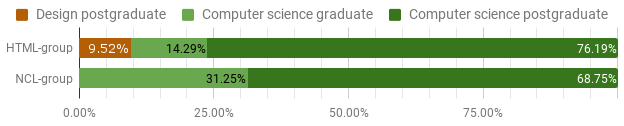
\includegraphics[width=10cm, keepaspectratio]{img/img16.png}
	\caption{Participants’ answers about their educational background.}
	\label{fig:profile1}
    \captionvspace
\end{center}
\end{figure}

\begin{figure}[!ht]
\begin{center}
	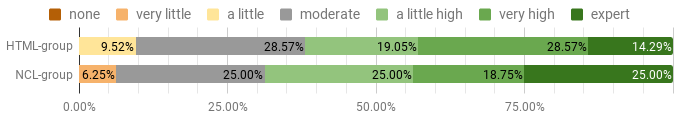
\includegraphics[width=10cm, keepaspectratio]{img/img17.png}
	\caption{Participants’ answers about their skill in their group language.}
	\label{fig:profile2}
    \captionvspace
\end{center}
\end{figure}

\begin{figure}[!ht]
\begin{center}
	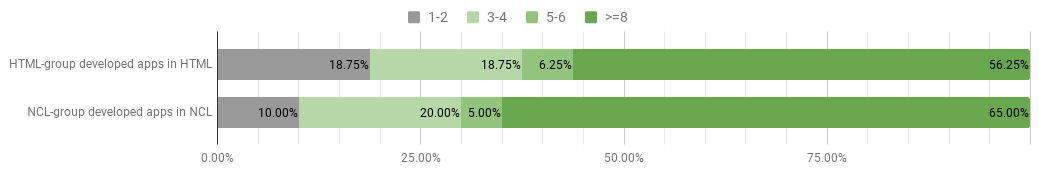
\includegraphics[width=14cm, keepaspectratio]{img/img18.png}
	\caption{Participants’ answers about the number of development applications 
	in their main language.}
	\label{fig:profile3}
    \captionvspace
\end{center}
\end{figure}


\begin{figure}[!ht]
\begin{center}
	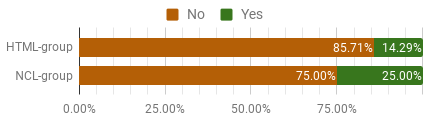
\includegraphics[width=8cm, keepaspectratio]{img/img19.png}
	\caption{Participants’ answers about whether they had developed multimodal 
	applications.}
    \captionvspace
	\label{fig:profile4}
\end{center}
\end{figure}

\subsection{Results about block-based representations}
\label{sec:evaluation:blocks-res}

Page 4 of the evaluation form presents the block-based representation and is
organized in four sections; each one presents a few concepts, followed by a
task.

\begin{itemize}
	\item Concepts 1.1: Presents the \textit{Media} and \textit{Relationship}
	blocks and a usage example. The example is an application that presents a
	video, shows an image when the video reaches its credits, and the video may be
	repeated if a user selects the image.
	\item Task 1.1: Asks the participant to describe a hypervideo application
	presented in block representation, using \textit{Media} and
	\textit{Relationship} elements. The application presents a video, shows two
	images when the video reaches its credits, and navigates to a video if user
	select the one of the images.
	\item Concepts 1.2: Presents the \textit{Recognizer} block and a usage
	example. The example is a new version of Concepts 1.1, but the video will be
	repeated if a user uses a voice command.
	\item Task 1.2: Asks the participant to describe a new version of the
	hypervideo application from Task 1.1, which uses a \textit{Recognizer} block
	to enable video navigation by a voice command. 
	\item Concepts 1.3: Presents the \textit{CompoundCondition} block and a usage
	example. The example is a new version of Concepts 1.2, but the video will be
	repeated if a user uses a voice or a gesture command.
	\item Task 1.3: Asks the participant to develop a new version of the
	hypervideo application from Task 1.2, which uses a \textit{CompoundCondition}
	block to enable video navigation by a voice or a gesture command.
	\item Concepts 1.4: Presents the \textit{UserClass} block and a usage example.
	The example is a new version of Concepts 1.2, but the video will be repeated
	only if a specific user gives a voice command.
	\item Task 1.4: Asks the participant to develop a new version of the
	hypervideo application from Task 1.3, which uses \textit{UserClass} block to
	enable to video navigation by voice command from a specific user.
\end{itemize}

Regarding the aforementioned tasks, participants in both groups made few
mistakes in both description (\fig{fig:blocks-res1}) and creation tasks
(\fig{fig:blocks-res2}). 

The answers for description tasks were classified as: “correct description”,
when the participant provided a correct description with some level of detail
(four or more sentences); “correct description with minor errors” when the
participant provided a correct description with some level of detail, but
missing some information, such as describing the end (stop) of an image or a
recognizer; and “generic description”, when the participant provided a correct
description but in general form (one or two sentences), which prevents us from
capturing any error.

\begin{figure}[!ht]
\begin{center}
	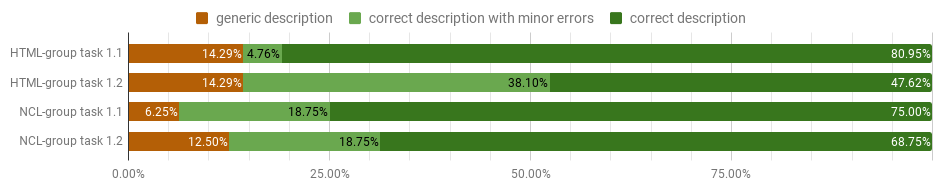
\includegraphics[width=14cm, keepaspectratio]{img/img20.png}
    \captionvspace
	\caption{Participants’ answers in the blocks-based tasks 1.1 and 1.2.}
	\label{fig:blocks-res1}
    \captionvspace
\end{center}
\end{figure}

The answers for the creation tasks were classified as: “correct”, when the
participant correctly made the required block changes; “correct block but with
mirror errors”, when the participant made errors such as forgetting to stop or
start some recognizer, or kept using the selection interaction; and “fail”, when
the changes did not solve what was asked.

\begin{figure}[!ht]
\begin{center}
	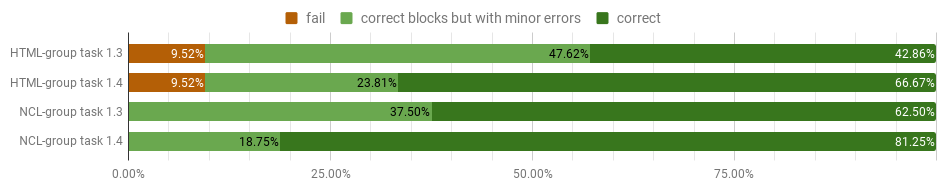
\includegraphics[width=14cm, keepaspectratio]{img/img21.png}
    \captionvspace
	\caption{Participants’ answers in the blocks-based tasks 1.3 and 1.4.}
	\label{fig:blocks-res2}
    \captionvspace
\end{center}
\end{figure}

Page 5 asks the participants’ opinion on TAM statements, as follows. 	
\fig{fig:blocks-res3} illustrates the participants’ answers.

\begin{itemize}
	\item PU 1: “The concepts presented allow to quickly specify multimodal
	applications.”
	\item PU 2: “The concepts presented allow you to specify multimodal
	applications with quality.”
	\item PU 3: “In general, the concepts presented are useful for specifying
	multimodal applications.”
	\item PEU 1: “The concepts presented are simple and understandable.”
	\item PEU 2: “The concepts presented are easy to learn.”
	\item PEU 3: “In general, the concepts presented are easy to use.”
\end{itemize}

\begin{figure}[!ht]
\begin{center}
	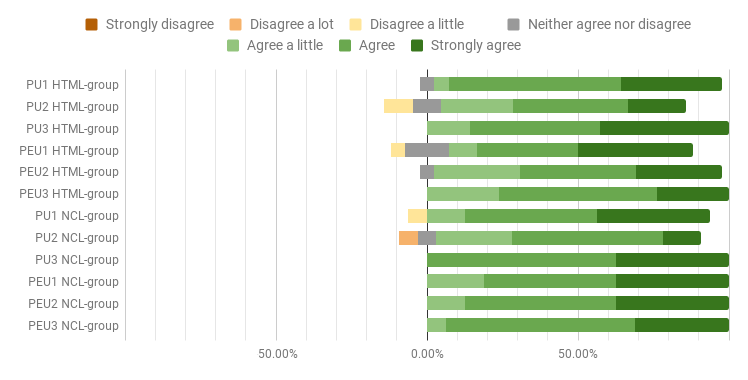
\includegraphics[width=14cm, keepaspectratio]{img/img22.png}
    \captionvspace
	\caption{Participants’ TAM answers about the block-based representation.}
    \captionvspace
	\label{fig:blocks-res3}
\end{center}
\end{figure}

\subsection{Results about extended language}
\label{sec:evaluation:lang-res}

Page 6 presents the syntax representations for the participant’s group language.
It is organized in four sections; each one presents concepts, followed by a
task.

\begin{itemize}
	\item Concepts 2.1: Presents \textit{Media} and \textit{Relationship} elements
	in the extended language syntax and a usage example. The usage example is the
	same as the one in Concepts 1.1. 
	\item Task 2.1: Asks the participant to describe a hypervideo application
	presented in the extended language syntax, using \textit{Media} and 
	\textit{Relationship} elements. The application is the same as the one in Task
	1.1.
	\item Concepts 2.2: Presents \textit{Recognizer} in the extended language
	syntax and usage example. The usage example is the same as the one in Concepts
	1.2.
	\item Task 2.2: Asks the participant to describe a simple hypervideo
	application, now using a Recognizer in the extended language syntax. The
	application is the same as the one in Task 1.2.
	\item Concepts 2.3: Presents the \textit{CompoundCondition} in the extended
	language syntax and a usage example. The usage example is the same as the one
	in Concepts 1.3.
	\item Tasks 2.3: Asks the participant to develop a new hypervideo application
	in the extended language syntax, now using a \textit{Recognizer} and a 
	\textit{CompoundCondition}. The application is the same as the one in Task
	1.3.
	\item Concepts 2.4: Presents \textit{UserClass} in the extended language
	syntax and a usage example. The usage example is the same as the one in
	Concepts 1.4.
	\item Tasks 2.4: Asks the participant to develop a new hypervideo application,
	now using a \textit{UserClass} in the extended language syntax. The
	application is the same as the one in Task 1.4.
\end{itemize}

Regarding the tasks, participants in both groups made few mistakes in both
description (\fig{fig:lang-res1}) and creation tasks (\fig{fig:lang-res2}).

\begin{figure}[!ht]
\begin{center}
	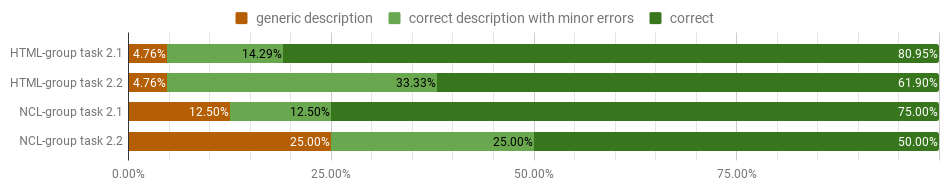
\includegraphics[width=14cm, keepaspectratio]{img/img23.png}
    \captionvspace
	\caption{Participants’ answers in the extended language tasks 2.1 and 2.2}
    \captionvspace
	\label{fig:lang-res1}
\end{center}
\end{figure}

\begin{figure}[!ht]
\begin{center}
	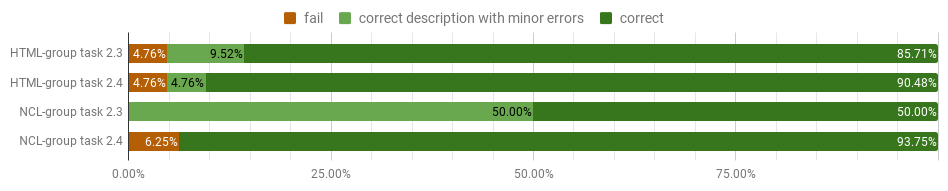
\includegraphics[width=14cm, keepaspectratio]{img/img24.png}
    \captionvspace
	\caption{Participants’ answers in the extended language tasks 2.3 and 2.4.}
    \captionvspace
	\label{fig:lang-res2}
\end{center}
\end{figure}

Page 7 asks the participants’ opinion on TAM statements, as follows. 
\fig{fig:lang-res3} illustrates the participants’ answers.

\begin{itemize}
	\item PU 1: “The extended language allows rapid development of multimodal
	applications.”
	\item PU 2: “The extended language allows the development of multimodal
	applications with quality.”
	\item PU 3: “In general, the extended language is useful for the development
	of multimodal applications.”
	\item PEU 1: “The extended language is simple and understandable.”
	\item PEU 2: “The extended language is easy to learn.”
	\item PEU 3: “Overall, the extended language is easy to use.”
\end{itemize}

\begin{figure}[!ht]
\begin{center}
	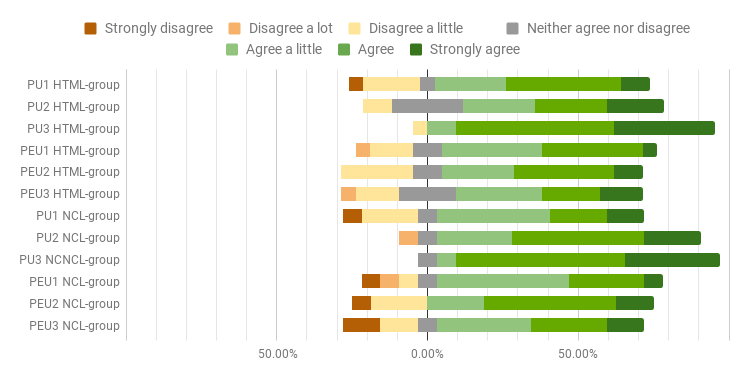
\includegraphics[width=14cm, keepaspectratio]{img/img25.png}
    \captionvspace
	\caption{Participants’ TAM answers about the extended language.}
    \captionvspace
	\label{fig:lang-res3}
\end{center}
\end{figure}

Finally, we asked their opinion regarding the quality of our instantiation with
the statement “The concepts presented in the previous section are clearly
instantiated in the extended language”. \fig{fig:lang-res4} illustrates the
participants’ answers.

\begin{figure}[!ht]
\begin{center}
	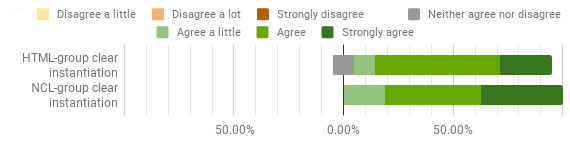
\includegraphics[width=10cm, keepaspectratio]{img/img26.png}
	\caption{Participants’ answers about the concepts instantiation.}
    \captionvspace
	\label{fig:lang-res4}
\end{center}
\end{figure}

\section{Discussion}
\label{sec:evaluation:discussion}

First, we must highlight that we have not found a relation between the users who
had not developed multimodal applications and the ones who performed the tasks
with errors. Also, we have not found relation between users who self-reported to
have lower knowledge of their group language and the ones who performed the
extended language tasks with errors.

If participants had performed the tasks with more errors, it might indicate that
they had not clearly understood the proposed entities and their TAM answer would
not be very informative. However, in general, both NCL and HTML participants
performed the tasks, on both block-based and extended language representations,
with few errors, so their TAM answers can be considered valuable.

Regarding the task identification errors, the most common ones were related with
missing the stop or start of some recognizer. This issue may be related with the
fact that NCL and HTML currently support mouse/key interactions through some
callback function (\textit{e.g.} onclick and onSelection), which do not need to be
activated or deactivated, unlike a recognizer.

Although most users said that the entities were clearly instantiated
(\fig{fig:lang-res4}), their answers to the TAM questions showed a little
difference between the block-based and extended languages representations. The
participants gave some slightly more positive answers for the block-based ones.
To understand why this was the case we need to conduct further studies. 

%%%%%%%%%%%%%%%%%%%%%%%%%%%%%%%%%%%%%%%%%%%%%%%%%%%%%%%%%%%%%%%%%%%%%%%%%%%%%%%%
\chapter{Final Remarks}
%%%%%%%%%%%%%%%%%%%%%%%%%%%%%%%%%%%%%%%%%%%%%%%%%%%%%%%%%%%%%%%%%%%%%%%%%%%%%%%%
\label{chp:final}

On the one hand, the studies performed by the multimedia research community has
resulted in multimedia-oriented programming languages, such as HTML, SMIL, and
NCL, which focus on the synchronization of audiovisual modalities (\textit{e.g.} text,
graphics, and videos) and GUI-based (keyboard and mouse) input modalities. On
the other hand, the studies performed by the multimodal interaction research
community have resulted in programming languages and frameworks that support the
development of MUIs. In general, however, the languages and frameworks proposed
by either community suffer some relevant drawbacks (discussed in 
\sect{sec:state:drawbacks}).
In this thesis, we propose to extend multimedia languages to support both
multimodal and multiuser interactions. We believe that these extensions can
contribute to the state of the art by overcoming the drawbacks and same time
increasing multimodal specification expressiveness.

A multimedia language that follows our model should instantiate as first-class 
citizens our proposed entities, i.e. \textit{Media}, \textit{Recognizer}, 
\textit{Relationship} and \textit{UserClass}. By so doing, these enable their 
developers also handle both fusion and fission processes, thus, 
prevents\textit{ the strong encapsulation between fusion and fission}. 
Moreover, the multimedia language will also support modality selection based on 
the user’s sensory capabilities and specification of interacting users, and the 
association of a user with recognition events. We discuss in 
\sect{chp:instantiation} the instantiation of the model entities into the NCL 
and HTML languages though new elements their syntax. 

Besides overcoming the above drawbacks, our proposal also achieves more
expressiveness when combining both output and input modalities. It does so by
using the causal relationship and anchor concepts from NCM. Those concepts
enable NCM express Allen’s temporal relations among output modalities. In our
approach, we enable such concepts for input modalities which enable it express
Allen’s temporal relations among both output modalities and input modalities.

To evaluate our approach, we perform an evaluation study comprised 37 
participants. We organize them into two groups based on their self-assessment 
of their knowledge of NCL and HTML. We organize them as 21 participants in the 
HTML group and 16 in the NCL group. This study was performed made it in two 
parts. The first part focuses on the conceptual entities, whereas the second 
part focuses on our proposed syntaxes for HTML and NCL. The first part about 
the conceptual entities was a challenge, because those entities were created to 
be independent from representation syntax. To do so, we used a block-based 
programing paradigm to enable users to develop applications using only the 
concept entities, at a level of abstraction higher than that of either NCL or 
HTML.

In both parts of the evaluation study, we presented the concepts entities and aiming at capture evidences of understanding and acceptance. To capture evidences of understanding, we ask developers answers coding tasks. To captures evidences of acceptance we use TAM based questionnaires. Both NCL and HTML participants, in general, performed the tasks with feel errors, which may indicate that they had reasonably understood, and they presents good acceptance in their answers to TAM questions.

\section{Publications}
\label{sec:publications}

Until the present moment, we archive the following
publications. In particular, those publications discuss the development of envisaged scenarios in NCL, varying the modalities and interacting users.

\begin{itemize}
	\item	 A. L. V. Guedes, R. G. de A. Azevedo, M. F. Moreno, and L. F. G.
	Soares, “Specification of Multimodal Interactions in NCL,” in Proceedings of
	the 21st Brazilian Symposium on Multimedia and the Web, New York, NY, USA,
	2015, pp. 181–187~\cite{guedes_specification_2015}.
	\item	A. L. V. Guedes, “Towards Supporting Multimodal and Multiuser
	Interactions in Multimedia Languages,” in In: Doctoral Consortium. Proceedings
	of the 2016 ACM Symposium on Document Engineering, New York, NY, USA,
	2016~\cite{guedes_towards_2016}.
	\item	A. L. V. Guedes, R. G. de A. Azevedo, and Simone Diniz Junqueira
	Barbosa, “Extending multimedia languages to support multimodal user
	interactions,” Multimed Tools Appl, pp. 1–30, Oct. 2016
	~\cite{guedes_extending_2016}.
	\item	A. L. V. Guedes, R. G. de Albuquerque Azevedo, S. Colcher, and S. D. J.
	Barbosa, “Extending NCL to Support Multiuser and Multimodal Interactions,” in
	Proceedings of the 22Nd Brazilian Symposium on Multimedia and the Web, New
	York, NY, USA, 2016, pp. 39–46~\cite{guedes_extending_2016-1}.
	\item	A. L. V. Guedes, Marcio Cunha, Hugo Fuks, Sérgio Colcher, and Simone
	Diniz Junqueira Barbosa, “Using NCL to Synchronize Media Objects, Sensors and
	Actuators,” in In: Workshop Internacional de Sincronismo das Coisas (WSoT), 1,
	2016, Teresina. Anais do XXII Simpósio Brasileiro de Sistemas Multimídia e
	Web. Porto Alegre: Sociedade Brasileira de Computação, 2016. v. 2, New York,
	NY, USA, 2016~\cite{guedes_using_2016}.	

\end{itemize}

\section{Future Works}
\label{sec:future}

As future work, we first aim at improving our proposal following two main paths.

First, we aim to investigate how to integrate higher-level constructions for
dialog management into our proposal. For instance, this could be achieved
through mappings from the form-based or state machine-based constructions onto
our conditions and actions. In particular, the mapping of these higher-level
constructs would generate stop/start of Recognizer elements, which participants
often missed in our evaluation.

Second, we aim to implement a system that fulfill the execution requirements
(discussed in \sect{sec:intro:scenarios}) and develop more usage scenarios. In 
particular, since NCL is an international standard for DTV, an NCL-based system 
may be used to exploit new kinds of applications in the DTV domain. It allows 
to go beyond the limited interaction (\textit{e.g.} remote control) and 
audiovisual media currently supported in this domain. Example of applications 
that can take advantages of our proposal include: (1) accessibility 
applications for disabled people or for the elderly; (2) educational 
applications for kids, like interactive classes of language or math; (3) 
immersive applications using different sensors and actuators. 

Following the above paths, we also aim at investigating the development of
multimedia applications with multimodal interaction features for mobile and
ubiquitous environments. Most mobile devices have sensor technologies —such as
accelerometer, compass, and geographic location— and actuators —such as
vibration motors. These devices can be useful for many kinds of multimodal user
interactions in multimedia applications.

Moreover, the development of graphical abstractions for multimedia authoring
with multimodal interactions is also necessary. Graphical tools offer an
alternative to editing XML code, which is often tedious and error prone; for
instance, a graphical editor could help in expressing complex temporal relations
between modalities. In particular, we can also improve our block-based
representation. It can be only both a standalone tool that generate NCL/HTML
code or be integrated some in authoring tool for one those languages. For
instance, NCL Composer~\cite{azevedo_composer:_2014} can use the block-based
presentation as an authoring view.

%%%%%%%%%%%%%%%%%%%%%%%%%%%%%%%%%%%%%%%%%%%%%%%%%%%%%%%%%%%%%%%%%%%%%%%%%%%%%%%%
% bibliography
%%%%%%%%%%%%%%%%%%%%%%%%%%%%%%%%%%%%%%%%%%%%%%%%%%%%%%%%%%%%%%%%%%%%%%%%%%%%%%%%
{ \footnotesize 
 	\arial
 	\bibliography{library}
}
\normalfont
\appendix

%%%%%%%%%%%%%%%%%%%%%%%%%%%%%%%%%%%%%%%%%%%%%%%%%%%%%%%%%%%%%%%%%%%%%%%%%%%%%%%%
\chapter{NCL Schemas}
%%%%%%%%%%%%%%%%%%%%%%%%%%%%%%%%%%%%%%%%%%%%%%%%%%%%%%%%%%%%%%%%%%%%%%%%%%%%%%%%
\label{annex:schemas}

In this appendix, we present five XML schemas from NCL 3.0\footnotemark~with 
our proposed extensions. The first one, illustrated in \lis{list:annexa1}, is a 
new schema  called NCL30Input.xsd, which includes our <input> element. The 
second one,  illustrated in \lis{list:annexa2}, is a new schema called 
NCL30UserClass.xsd,  which  includes our <userClass> element. The renaming 
schemas are modified  versions of existing ones from the NCL 3.0 (changes are 
highlighted in light  green), to include our extensions to link-related 
elements. The third schema, illustrated in \lis{list:annexa3}, is a modified 
version of the NCL30ConnectorCommonPart.xsd. The fourth schema, illustrated in 
\lis{list:annexa4}, is an extended version of 
the NCL30ConnectorCausalExpression.xsd. Finally, the fifth schema, illustrated 
in \lis{list:annexa5}, is a modified version of the NCL30Linking.xsd.

\footnotetext{\url{https://github.com/TeleMidia/ncl30-schemas/}}


\begin{listing}[!ht]
\begin{minted}[linenos,fontsize=\scriptsize,numbersep=1pt,frame=lines,xleftmargin=10pt,framesep=2mm,]{xml}
<schema xmlns="http://www.w3.org/2001/XMLSchema"
  xmlns:input="http://www.ncl.org.br/NCL3.0/Input"
  targetNamespace="http://www.ncl.org.br/NCL3.0/Input"
  elementFormDefault="qualified" attributeFormDefault="unqualified">
  <complexType name="inputPrototype">
    <attribute name="id" type="ID" use="required"/>
    <attribute name="type" type="string" use="optional"/>
    <attribute name="src" type="anyURI" use="optional"/>
  </complexType>
  <element name="input" type="input:inputPrototype"/>
</schema>
\end{minted}
\caption{New NCL30Input.xsd.}
\label{list:annexa1}
\end{listing}

\begin{listing}[!ht]
\begin{minted}[linenos,fontsize=\scriptsize,numbersep=1pt,frame=lines,xleftmargin=10pt,framesep=2mm]{xml}
<schema xmlns="http://www.w3.org/2001/XMLSchema"
  xmlns:userclass="http://www.ncl.org.br/NCL3.0/UserClass"
  targetNamespace="http://www.ncl.org.br/NCL3.0/UserClass "
  elementFormDefault="qualified" attributeFormDefault="unqualified">
  <complexType name="userClassPrototype">
    <attribute name="id" type="ID" use="required"/>
    <attribute name="min" type="positiveInteger" use="required"/>
    <attribute name="max" type="positiveInteger" use="required"/>
    <attribute name="src" type="anyURI" use="required"/>
  </complexType>
  <element name="userClass" type="userClass:userClassPrototype"/>
</schema>
\end{minted}
\caption{New NCL30UserClass.xsd.}
\label{list:annexa2}
\end{listing}

\begin{listing}[!ht]
\begin{minted}[linenos,fontsize=\scriptsize,numbersep=1pt,frame=lines,xleftmargin=10pt,framesep=2mm,
 highlightlines={8,9,17,24}]{xml}
<schema xmlns="http://www.w3.org/2001/XMLSchema"
  xmlns:connectorCommonPart="http://www.ncl.org.br/NCL3.0/ConnectorCommonPart"
  targetNamespace="http://www.ncl.org.br/NCL3.0/ConnectorCommonPart"
  elementFormDefault="qualified" attributeFormDefault="unqualified">
  <complexType name="parameterPrototype">
    <attribute name="name" type="string" use="required"/>
    <attribute name="type" type="string" use="optional"/>
    <attribute name="component" type="IDREF" use="optional"/>
    <attribute name="interface" type="string" use="optional"/>
  </complexType>
  <simpleType name="eventPrototype">
    <restriction base="string">
      <enumeration value="presentation" />
      <enumeration value="selection" />
      <enumeration value="attribution" />
      <enumeration value="composition" />
      <enumeration value="recognition" />
    </restriction>
  </simpleType>
  <simpleType name="logicalOperatorPrototype">
    <restriction base="string">
      <enumeration value="and" />
      <enumeration value="or" />
      <enumeration value="seq" />
    </restriction>
  </simpleType>
  <simpleType name="transitionPrototype">
    <restriction base="string">
      <enumeration value="starts" />
      <enumeration value="stops" />
      <enumeration value="pauses" />
      <enumeration value="resumes" />
      <enumeration value="aborts" />
    </restriction>
  </simpleType>
</schema>
\end{minted}
\caption{Extended NCL30ConnectorCommonPart.xsd.}
\label{list:annexa3}
\end{listing}

\begin{listing}[t]
\begin{minted}[linenos,fontsize=\scriptsize,numbersep=1pt,frame=topline,xleftmargin=10pt,framesep=2mm, highlightlines={19}]{xml}
<schema xmlns="http://www.w3.org/2001/XMLSchema"      
  xmlns:connectorCausalExpression="http://www.ncl.org.br/NCL3.0/ConnectorCausalExpression"
  xmlns:connectorCommonPart="http://www.ncl.org.br/NCL3.0/ConnectorCommonPart"
  targetNamespace="http://www.ncl.org.br/NCL3.0/ConnectorCausalExpression"
  elementFormDefault="qualified" attributeFormDefault="unqualified">
  <import namespace="http://www.ncl.org.br/NCL3.0/ConnectorCommonPart"
  schemaLocation="http://www.ncl.org.br/NCL3.0/modules/NCL30ConnectorCommonPart.xsd"/>
  <simpleType name="conditionRoleUnion">
    <union memberTypes="string
    connectorCausalExpression:conditionRolePrototype"/>
  </simpleType>
  <simpleType name="conditionRolePrototype">
    <restriction base="string">
      <enumeration value="onBegin" />
      <enumeration value="onEnd" />
      <enumeration value="onPause" />
      <enumeration value="onResume" />
      <enumeration value="onAbort" />
      <enumeration value="onRecognize" />
    </restriction>
  </simpleType>
  <simpleType name="maxUnion">
    <union memberTypes="positiveInteger
    connectorCausalExpression:unboundedString"/>
  </simpleType>
  <simpleType name="unboundedString">
    <restriction base="string">
      <pattern value="unbounded"/>
    </restriction>
  </simpleType>
\end{minted}
\end{listing}

\begin{listing}[t]
\begin{minted}[linenos,fontsize=\scriptsize,numbersep=1pt,frame=none,xleftmargin=10pt,framesep=2mm, firstnumber=31, highlightlines={36,37}]{xml}
  <complexType name="simpleConditionPrototype">
    <attribute name="role" type="connectorCausalExpression:conditionRoleUnion" 
      use="required"/>
    <attribute name="eventType" type="connectorCommonPart:eventPrototype" 
      use="optional"/>
    <attribute name="user_id" type="string" use="optional"/>
    <attribute name="excluded_user_id" type="string" use="optional"/>
    <attribute name="key" type="string" use="optional"/>
    <attribute name="transition" type="connectorCommonPart:transitionPrototype" 
      use="optional"/>
    <attribute name="delay" type="string" use="optional"/>
    <attribute name="min" type="positiveInteger" use="optional"/>
    <attribute name="max" type="connectorCausalExpression:maxUnion" 
      use="optional"/>
    <attribute name="qualifier" 
      type="connectorCommonPart:logicalOperatorPrototype" use="optional"/>
  </complexType>
  <complexType name="compoundConditionPrototype">
    <attribute name="operator" 
      type="connectorCommonPart:logicalOperatorPrototype" use="required"/>
    <attribute name="delay" type="string" use="optional"/>
  </complexType>
  <simpleType name="actionRoleUnion">
    <union memberTypes="string connectorCausalExpression:actionNamePrototype"/>
  </simpleType>
  <simpleType name="actionNamePrototype">
    <restriction base="string">
      <enumeration value="start" />
      <enumeration value="stop" />
      <enumeration value="pause" />
      <enumeration value="resume" />
      <enumeration value="abort" />
      <enumeration value="set" />
    </restriction>
  </simpleType>
  <simpleType name="actionOperatorPrototype">
    <restriction base="string">
      <enumeration value="par" />
      <enumeration value="seq" />
    </restriction>
  </simpleType>
  <complexType name="simpleActionPrototype">
    <attribute name="role" type="connectorCausalExpression:actionRoleUnion"     
      use="required"/>
    <attribute name="eventType" type="connectorCommonPart:eventPrototype" 
      use="optional"/>
    <attribute name="actionType"
      type="connectorCausalExpression:actionNamePrototype" use="optional"/>
    <attribute name="delay" type="string" use="optional"/>
    <attribute name="value" type="string" use="optional"/>
    <attribute name="repeat" type="positiveInteger" use="optional"/>
    <attribute name="repeatDelay" type="string" use="optional"/>
    <attribute name="min" type="positiveInteger" use="optional"/>
    <attribute name="max" type="connectorCausalExpression:maxUnion" 
      use="optional"/>
    <attribute name="qualifier" 
      type="connectorCausalExpression:actionOperatorPrototype" use="optional"/>
  </complexType>
  
\end{minted}
\end{listing}

\begin{listing}[!ht]
\begin{minted}[linenos,fontsize=\scriptsize,numbersep=1pt,frame=bottomline,xleftmargin=10pt,framesep=2mm]{xml}
  <complexType name="compoundActionPrototype">
    <choice minOccurs="2" maxOccurs="unbounded">
      <element ref="connectorCausalExpression:simpleAction" />
      <element ref="connectorCausalExpression:compoundAction" />
    </choice>
    <attribute name="operator" 
      type="connectorCausalExpression:actionOperatorPrototype" use="required"/>
    <attribute name="delay" type="string" use="optional"/>
  </complexType>
  <element name="simpleCondition" 
    type="connectorCausalExpression:simpleConditionPrototype" />
  <element name="compoundCondition"  
    type="connectorCausalExpression:compoundConditionPrototype" />
  <element name="simpleAction"  
    type="connectorCausalExpression:simpleActionPrototype" />
  <element name="compoundAction"  
    type="connectorCausalExpression:compoundActionPrototype" />
</schema>
\end{minted}
\caption{Extended NCL30ConnectorCausalExpression.xsd.}
\label{list:annexa4}
\end{listing}

\begin{listing}[!ht]
\begin{minted}[linenos,fontsize=\scriptsize,numbersep=1pt,frame=lines,xleftmargin=10pt,framesep=2mm,
 highlightlines={8,9}]{xml}
  <schema xmlns="http://www.w3.org/2001/XMLSchema"
  xmlns:linking="http://www.ncl.org.br/NCL3.0/Linking"
  targetNamespace="http://www.ncl.org.br/NCL3.0/Linking"
  elementFormDefault="qualified" attributeFormDefault="unqualified">
  <complexType name="paramPrototype">
    <attribute name="name" type="string" use="required"/>
    <attribute name="value" type="anySimpleType" use="required"/>
    <attribute name="component" type="IDREF" use="required"/>
    <attribute name="interface" type="string" use="optional"/>
  </complexType>
  <complexType name="bindPrototype">
    <sequence minOccurs="0" maxOccurs="unbounded">
      <element ref="linking:bindParam"/>
    </sequence>
    <attribute name="role" type="string" use="required"/>
    <attribute name="component" type="IDREF" use="required"/>
    <attribute name="interface" type="string" use="optional"/>
  </complexType>
  <complexType name="linkPrototype">
    <sequence>
      <element ref="linking:linkParam" minOccurs="0" maxOccurs="unbounded"/>
      <element ref="linking:bind" minOccurs="2" maxOccurs="unbounded"/>
    </sequence>
    <attribute name="id" type="ID" use="optional"/>
    <attribute name="xconnector" type="string" use="required"/>
  </complexType>
  <element name="linkParam" type="linking:paramPrototype"/>
  <element name="bindParam" type="linking:paramPrototype"/>
  <element name="bind" type="linking:bindPrototype" />
  <element name="link" type="linking:linkPrototype" />
</schema>
\end{minted}
\caption{ Extended NCL30Linking.xsd.}
\label{list:annexa5}
\end{listing}

%%%%%%%%%%%%%%%%%%%%%%%%%%%%%%%%%%%%%%%%%%%%%%%%%%%%%%%%%%%%%%%%%%%%%%%%%%%%%%%%
\chapter{NCL Envisaged Scenarios}
%%%%%%%%%%%%%%%%%%%%%%%%%%%%%%%%%%%%%%%%%%%%%%%%%%%%%%%%%%%%%%%%%%%%%%%%%%%%%%%%
\label{annex:scenarios}

In this appendix, we present three of the envisaged scenarios using our extended
NCL syntax, namely: “Put-that-there”, “I-Get-That-You-Put-It-There” and
“Anyone-Get-That-Someone-Else-Put-It-There”. They enable users to move an image
(the Ginga logo) using a combination of voice and gesture commands. To enable
voice interactions, the scenarios use the same description files, namely
“sentences.ssml” (\lis{list:annexb1}) and “commands.srgs” 
(\lis{list:annexb2}).

\begin{listing}[h]
\begin{minted}[linenos,fontsize=\scriptsize,numbersep=1pt,frame=lines,xleftmargin=10pt,framesep=2mm]{xml}
<speak xmlns="http://www.w3.org/2001/10/synthesis">
  <s id="repeat_question">where?</s>
</speak>
\end{minted}
\caption{sentences.ssml.}
\label{list:annexb1}
\end{listing}

\begin{listing}[h]
\begin{minted}[linenos,fontsize=\scriptsize,numbersep=1pt,frame=lines,xleftmargin=10pt,framesep=2mm]{xml}
<grammar xmlns="http://www.w3.org/2001/06/grammar">
  <rule id="put_that">put that</rule>
  <rule id="there">there</rule>
</grammar>
\end{minted}
\caption{commands.sgrs.}
\label{list:annexb2}
\end{listing}

\lis{list:annexb3} presents the NCL code of <media>, <input> and <ports>
elements shared among the scenarios. Those scenarios only differ by the used
<link> elements (discussed next). The <media> elements (lines 4-9) are “logo”,
which define the movable image, and “sentences”, which define the speech
feedback using “sentences.ssml”. An <area> element is defined in the “sentences”
pointing to the SSML fragment responsible for defining the word “where”. The
<input> elements (lines 10-19) are “pointer” input, responsible for recognizing
the point on the screen at which the user’s finger is pointing, and “asr” input,
to enable voice commands using the “commands.sgrs” file. Two anchors are defined
in “asr”, pointing to SRGS rules with the ids “put that” and “there”. Both
scenarios begin by starting the “logo”, “pointer”, and “asr” elements, as
defined in the <port> elements (lines 1-3). In particular, the “asr” media is
started by the “put\_that” interface, which defines the word expected in the
first interaction.

\begin{minted}[linenos,fontsize=\scriptsize,numbersep=1pt,frame=lines,xleftmargin=10pt,framesep=2mm]{xml}
<port component="icon"/>
<port component="pointer"/>
<port component="asr" interface="put_that"/>
<media id="icon" src="ginga.png">
  <property name="location" value="20%, 20%"/>
</media>
<media id="sentences" src="sentences.ssml">
  <area label="where"/>
</media>
<input id="pointer" type="application/x-ncl-pointer">
  <area label="move"/>
  <property name="x"/>
  <property name="y"/>
</input>
<input id="asr" type="application/srgs+xml" src="commands.sgrs">
  <property name="userClass" name="BoltLikeUser"/>
  <area label="put_that"/>
  <area label="there"/>
</input>
\end{minted}
\captionvspace
\begin{listing}[!ht]
\caption{Used <media>, <input> and <port> elements in the three scenarios.}
\label{list:annexb3}
\end{listing}

The first scenario, “Put-that-there”, requires two <link> elements, which use
the new “recognition” event, both illustrated in \label{list:annexb4}. The first
<link> defines that when the application recognizes a “put that” voice command,
followed by the selection of the “logo” media, it will synthesize the word
“where” and expect a “there” voice command. The second <link> defines that when
the application recognize a “there” voice command, followed by a move of the
pointer, the “logo” must be moved to the new position at which the user’s finger
is pointing.

\begin{minted}[linenos,fontsize=\scriptsize,numbersep=1pt,frame=lines,xleftmargin=10pt,framesep=2mm]{xml}
<ncl xmlns="http://www.ncl.org.br/NCL3.0/EDTVProfile">
  <head>
    <connectorBase>
      <causalConnector id="onRecognizeSEQonSelectionStart">
        <compoundCondition operator="seq">
          <simpleCondition role="onSelection"/>
          <simpleCondition role="onRecognize"/>
        </compoundCondition>
        <simpleAction role="start"/>
      </causalConnector>
      <causalConnector id="onRecognizeSet">
        <connectorParam name="varSet"/>
        <simpleCondition role="onRecognize" qualifier="seq"/>
        <simpleAction role="set" value="$varSet"/>
      </causalConnector>
    </connectorBase>
  </head>
  <body>
    ... <!--### code from Listing 16 ###-->
    <link xconnector="onRecognizeSEQonSelectionStart">
      <bind role="onRecognize" component="asr" interface="put_that"/>
      <bind role="onSelection" component="icon"/>
      <bind role="start" component="sentences" interface="where"/>
      <bind role="start" component="asr" interface="there"/>
    </link>
    <link xconnector="onRecognizeSet">
      <bind role="onRecognize" component="asr" interface="there"/>
      <bind role="onRecognize" component="pointer" interface="move"/>
      <bind role="getValueX" component="pointer" interface="x"/>
      <bind role="getValueY" component="pointer" interface="y"/>
      <bind role="set" component="icon" interface="left">
        <bindParam name="varSet" value="$getValueX"/>
      </bind>
      <bind role="set" component="icon" interface="top">
        <bindParam name="varSet" value="$getValueY"/>
      </bind>
    </link>
  </body>
</ncl>
\end{minted}
\captionvspace
\begin{listing}[!ht]
\caption{Code fragment of “Put-That-There” in NCL.}

\label{list:annexb4}
\end{listing}

The other two scenarios consider interactions of two distinct users. One user
selects the icon and the other one moves it. Both scenarios require that users
have a pointer and a microphone device. Such requirement is defined by the
“boltlikeuser.sparql” file, illustrated in \label{list:annexb5}.

\begin{listing}[!ht]
\begin{minted}[linenos,fontsize=\scriptsize,numbersep=1pt,frame=lines,xleftmargin=10pt,framesep=2mm]{sql}
PREFIX foaf: <http://xmlns.com/foaf/0.1/>
PREFIX prf: <http://www.wapforum.org/profiles/UAPROF/ccppschema-20010430>
SELECT ?person
WHERE {
 ?person foaf:mbox ?email FILTER regex(?email, "@inf.puc-rio.br$") .
 ?person prf:component ?component1 . ?component1 prf:name ?name1 .
 FILTER regex(?name1, "leapmotion") .
 ?person prf:component ?component2 .  ?component2 prf:name ?name2 .
 FILTER regex(?name2, "microphone")
}
\end{minted}
\caption{boltlikeuser.sparql.}
\label{list:annex5}
\end{listing}

The “I-Get-That-You-Put-It-There” scenario considers interactions from two
identified users. \label{list:annexb6} shows the code fragment of this scenario,
which uses a <userClass> element (lines 20-23) and modified versions of the
<link> elements from the previous scenario. The difference from previous <link>
elements use is the “user\_id” in <linkParam> to specify each interacting user.
In the <link> elements’ connectors, those “user\_id” attributes are used as
parameter for <simpleCondition>.

\begin{minted}[linenos,fontsize=\scriptsize,numbersep=1pt,frame=lines,xleftmargin=10pt,framesep=2mm]{xml}
  <ncl xmlns="http://www.ncl.org.br/NCL3.0/EDTVProfile">
  <head>
    <connectorBase>
      <causalConnector id="onRecognizeSEQonSelectionByUserStart">
        <connectorParam name="user_id"/>
        <compoundCondition operator="seq">
          <simpleCondition role="onRecognize" user_id="$user_id"/>
          <simpleCondition role="onSelection" user_id="$user_id"/>
        </compoundCondition>
        <simpleAction role="start"/>
      </causalConnector>
      <causalConnector id="onRecognizeByUserSet">
        <connectorParam name="user_id"/>
        <connectorParam name="varSet"/>
        <simpleCondition role="onRecognize" qualifier="seq" 
          user_id="$user_id" />
        <simpleAction role="set" value="$varSet"/>
      </causalConnector>
    </connectorBase>
    <userBase>
      <userClass id="BoltLikeUser" min="2" max="2" 
        userClassDescription="boltlikeuser.sparql"/>
    </userBase>
  </head>
  <body>
    ... <!--### code from Listing 16 ###-->
    <link xconnector="onRecognizeSEQonSelectionByUserStart">
      <linkParam name="user_id" value="BoltLikeUser(1)"/>
      <bind role="onRecognize" component="asr" interface="put_that"/>
      <bind role="onSelection" component="icon"/>
      <bind role="start" component="sentences" interface="where"/>
      <bind role="start" component="asr" interface="there"/>
    </link>
    <link xconnector="onRecognizeSEQByUserSet">
      <linkParam name="user_id" value="BoltLikeUser(2)"/>
      <bind role="onRecognize" component="asr" interface="there"/>
      <bind role="onRecognize" component="pointer" interface="move"/>
      <bind role="getValueX" component="pointer" interface="x"/>
      <bind role="getValueY" component="pointer" interface="y"/>
      <bind role="set" component="icon" interface="left">
        <bindParam name="varSet" value="$getValueX"/>
      </bind>
      <bind role="set" component="icon" interface="top">
        <bindParam name="varSet" value="$getValueY"/>
      </bind>
    </link>
  </body>
</ncl>
\end{minted}
\begin{listing}[!ht]
\caption{Code fragment of “I-Get-That-You-Put-It-There”.}
\label{list:annexb6}
\end{listing}

Finally, the “Anyone-Get-That-Someone-Else-Put-It-There” scenario also considers
interactions of any two users, but not specified ones. More precisely, it first
expects the interaction of any user and, in sequence, the interaction of another
one, who must be different from the first one. To define this behavior, we split
the first <link> of previous scenarios in two links. \label{list:annexb7} shows
the code fragment of the three <link> elements, which are described in what
follows. 

The first <link> (lines 32-37) says that when any user perform the voice command
“put\_that”, we then store its “user\_id”. To get the “user\_id”, this <link>
uses our extended <linkParam> (lines 34-35) and <connectorParam> (lines 6-7).
The <connectorParam> access the “user\_id” from a “recognition” event of the
given interface passed in the <linkParam>. Then, the link sets the “user\_id”
value to a given role, which in our case is the SettingsNode.

The second <link> (lines 38-44) says that when the user, with the stored
“user\_id”, performs the selection of the “logo” media, the application will
synthesize the word “where” and expect a “there” voice command. To use the
stored “user\_id” in the <simpleCondtion> for the “onSelection” role, this
<link> also uses our extended <linkParam> (lines 39-40). 

Finally, the third <link> (lines 45-58) says that when another user performs the
voice command “there”, the “logo” must be moved to the new position at which
this user is pointing. Here, “another user” is defined by specifying
“excluded\_user\_id” in the <bindParam>, which is the value of the previously
stored “user\_id”, from the first interaction.

\begin{minted}[linenos,fontsize=\scriptsize,numbersep=1pt,frame=lines,xleftmargin=10pt,framesep=2mm]{xml}
<ncl xmlns="http://www.ncl.org.br/NCL3.0/EDTVProfile">
  <head>
    <connectorBase>
      <causalConnector id="onRecognizeSetUserId">
        <simpleCondition role="onRecognize"/>
        <connectorParam name="get_recognized_user" evenType="recognition" 
          attributeType="user_id"/>
        <simpleAction role="set" value="$get_recognized_user"/>
      </causalConnector>
      <causalConnector id="onSelectionByUserStart">
        <connectorParam name="user_id"/>
        <simpleCondition role="onSelection" user_id="$user_id"/>
        <simpleAction role="start"/>
      </causalConnector>
      <causalConnector id="onRecognizeByExcludedUserSet">
        <connectorParam name="excluded_user_id"/>
        <simpleCondition role="onRecognize" qualifier="seq" 
          excluded_user_id="$excluded_user_id"/>
        <simpleAction role="set"/>
      </causalConnector>
    </connectorBase>
    <userBase>
      <userClass id="BoltLikeUser" min="2" max="2" 
        userClassDescription="boltlikeuser.sparql"/>
    </userBase>
  </head>
  <body>
    ... <!--### code from Listing 16 ###-->
    <media id="settings" type="application/x-ncl-settings">
      <property name="first_user"/>
    </media>
    <link xconnector="onRecognizeSetUserId">
      <bind role="onRecognize" component="asr" interface="put_that"/>
      <linkParam name="get_recognized_user" component="asr" 
        interface="put_that"/>
      <bind role="set" component="settings" interface="first_user"/>
    </link>
    <link xconnector="onSelectionByUserStart">
      <linkParam name="user_id" component="settings"
         interface="first_user"/>
      <bind role="onSelection" component="logo"/>
      <bind role="start" component="sentences" interface="where"/>
      <bind role="start" component="asr" interface="there"/>
    </link>
    <link xconnector="onRecognizeByExcludedUserSet">
      <linkParam name="excluded_user_id" component="settings" 
        interface="first_user"/>
      <bind role="onRecognize" component="asr" interface="there"/>
      <bind role="onRecognize" component="pointer" interface="move"/>
      <bind role="getValueX" component="pointer" interface="x"/>
      <bind role="getValueY" component="pointer" interface="y"/>
      <bind role="set" component="icon" interface="left">
        <bindParam name="varSet" value="$getValueX"/>
      </bind>
      <bind role="set" component="icon" interface="top">
        <bindParam name="varSet" value="$getValueY"/>
      </bind>
    </link>
  </body>
</ncl>
\end{minted}
\begin{listing}[!ht]
\caption{Code fragment of “Anyone-Get-That-Someone-Else-Put-It-There”.}
\label{list:annexb7}
\end{listing}

%%%%%%%%%%%%%%%%%%%%%%%%%%%%%%%%%%%%%%%%%%%%%%%%%%%%%%%%%%%%%%%%%%%%%%%%%%%%%%%%
\chapter{Screenshots}
%%%%%%%%%%%%%%%%%%%%%%%%%%%%%%%%%%%%%%%%%%%%%%%%%%%%%%%%%%%%%%%%%%%%%%%%%%%%%%%%
\label{annex:screenshots}

Each section of this appendix presents screenshots of each page of the website
used in the evaluation study.

\section{Page 1 for all participants}

\newcounter{loop}
\forloop{loop}{1}{\value{loop}<2}{
    \begin{figure}[H]
    \begin{center}
    	\captionvspace
    	\includegraphics[width=14cm]{img-annex/img\arabic{loop}.png}
    	\captionvspace
    \end{center}
    \end{figure}
}

\section{Page 2 for all participants}

\forloop{loop}{2}{\value{loop}<4}{
\begin{figure}[ht]
\captionvspace
\begin{center}
	\includegraphics[width=14cm]{img-annex/img\arabic{loop}.png}
\end{center}
\captionvspace
\end{figure}
}

\section{Page 3 for all participants}

\forloop{loop}{4}{\value{loop}<6}{
\begin{figure}[H]
\captionvspace
\begin{center}
	\includegraphics[width=14cm]{img-annex/img\arabic{loop}.png}
\end{center}
\captionvspace
\end{figure}
}

\section{Page 4 for all participants}

\forloop{loop}{6}{\value{loop}<24}{
\begin{figure}[H]
\captionvspace
\begin{center}
	\includegraphics[width=14cm]{img-annex/img\arabic{loop}.png}
\end{center}
\captionvspace
\end{figure}
}

\section{Page 5 for all participants}

\forloop{loop}{24}{\value{loop}<27}{
\begin{figure}[H]
\captionvspace
\begin{center}
	\includegraphics[width=14cm]{img-annex/img\arabic{loop}.png}
\end{center}
\captionvspace
\end{figure}
}

\section{Page 6 for NCL participants}

\forloop{loop}{27}{\value{loop}<49}{
\begin{figure}[H]
\captionvspace
\begin{center}
	\includegraphics[width=14cm]{img-annex/img\arabic{loop}.png}
\end{center}
\captionvspace
\end{figure}
}

\section{Page 7 for NCL participants}

\forloop{loop}{49}{\value{loop}<53}{
\begin{figure}[H]
\captionvspace
\begin{center}
	\includegraphics[width=14cm]{img-annex/img\arabic{loop}.png}
\end{center}
\captionvspace
\end{figure}
}

\section{Page 6 for HTML participants}

\forloop{loop}{54}{\value{loop}<73}{
\begin{figure}[H]
\captionvspace
\begin{center}
	\includegraphics[width=14cm]{img-annex/img\arabic{loop}.png}
\end{center}
\captionvspace
\end{figure}
}

\section{Page 7 for HTML participants}

\forloop{loop}{73}{\value{loop}<76}{
\begin{figure}[H]
\captionvspace
\begin{center}
	\includegraphics[width=14cm]{img-annex/img\arabic{loop}.png}
\end{center}
\captionvspace
\end{figure}
}

\end{document}
